\documentclass[10pt,a4paper]{article}
\usepackage{paper_style}
\hypersetup{pdftitle={PHASE-TTC: From Motion to Time},pdfsubject={A Causal Event--RGB System for Signed Time-to-Contact Estimation}}
% Generated by scripts/make_official_results.py; do not edit by hand.
\providecommand{\OfficialPhasePublishedOverallMiD}{35.80}
\providecommand{\OfficialOverallAbsoluteGain}{9.228548419}
\providecommand{\OfficialBandContributionSubtotal}{9.227548419}
\providecommand{\OfficialDisplayRoundingResidual}{0.0010}
\providecommand{\OfficialCrucialSmallContributionShare}{82.4\%}
\providecommand{\OfficialPhaseOverallMiD}{35.8015}
\providecommand{\OfficialGarlOverallMiD}{45.03}
\providecommand{\OfficialOverallRelativeGain}{20.49\%}
\providecommand{\OfficialPhaseCrucialMiD}{43.5190}
\providecommand{\OfficialGarlCrucialMiD}{53.13}
\providecommand{\OfficialCrucialRelativeGain}{18.09\%}
\providecommand{\OfficialPhaseSmallMiD}{28.2568}
\providecommand{\OfficialGarlSmallMiD}{37.58}
\providecommand{\OfficialSmallRelativeGain}{24.81\%}
\providecommand{\OfficialPhaseLargeMiD}{25.7179}
\providecommand{\OfficialGarlLargeMiD}{40.61}
\providecommand{\OfficialLargeRelativeGain}{36.67\%}
\providecommand{\OfficialPhaseNegativeMiD}{29.9314}
\providecommand{\OfficialGarlNegativeMiD}{31.29}
\providecommand{\OfficialNegativeRelativeGain}{4.34\%}
\providecommand{\OfficialSampleCount}{6,762}
\providecommand{\OfficialPhaseFailureRate}{0.0\%}
\providecommand{\OfficialGarlFailureRate}{0.0\%}
\providecommand{\OfficialPhaseSubmissionID}{1016512}
\providecommand{\OfficialGarlSubmissionID}{817519}

% Generated by scripts/make_evttc_results.py. Do not edit manually.
\newcommand{\EvTTCQueryCount}{434}
\newcommand{\EvTTCSequenceCount}{10}
\newcommand{\EvTTCPredictionRowCount}{1,736}
\newcommand{\EvTTCPhaseFinite}{434}
\newcommand{\EvTTCPhaseCoverage}{434/434}
\newcommand{\EvTTCPhaseNegativeCount}{2}
\newcommand{\EvTTCPhasePredictionMin}{-42.225}
\newcommand{\EvTTCPhasePredictionMax}{51.869}
\newcommand{\EvTTCPhaseModelMedian}{0.753\,s}
\newcommand{\EvTTCPhaseModelPninetyfive}{7.820\,s}
\newcommand{\EvTTCPhaseCostMedian}{2.687\,s}
\newcommand{\EvTTCPhaseCostPninetyfive}{9.073\,s}
\newcommand{\EvTTCGarlFullFinite}{424}
\newcommand{\EvTTCGarlFullCoverage}{424/434}
\newcommand{\EvTTCGarlFullNegativeCount}{0}
\newcommand{\EvTTCGarlFullPredictionMin}{0.907}
\newcommand{\EvTTCGarlFullPredictionMax}{52.705}
\newcommand{\EvTTCGarlFullModelMedian}{0.039\,s}
\newcommand{\EvTTCGarlFullModelPninetyfive}{0.045\,s}
\newcommand{\EvTTCGarlFullCostMedian}{0.542\,s}
\newcommand{\EvTTCGarlFullCostPninetyfive}{1.009\,s}
\newcommand{\EvTTCGarlFullMedianDisagreement}{0.261\,s}
\newcommand{\EvTTCGarlFullPninetyfiveDisagreement}{1.098\,s}
\newcommand{\EvTTCGarlEventFinite}{434}
\newcommand{\EvTTCGarlEventCoverage}{434/434}
\newcommand{\EvTTCGarlEventNegativeCount}{10}
\newcommand{\EvTTCGarlEventPredictionMin}{-42.211}
\newcommand{\EvTTCGarlEventPredictionMax}{406.095}
\newcommand{\EvTTCGarlEventModelMedian}{0.007\,s}
\newcommand{\EvTTCGarlEventModelPninetyfive}{0.011\,s}
\newcommand{\EvTTCGarlEventCostMedian}{0.350\,s}
\newcommand{\EvTTCGarlEventCostPninetyfive}{0.806\,s}
\newcommand{\EvTTCGarlEventMedianDisagreement}{0.681\,s}
\newcommand{\EvTTCGarlEventPninetyfiveDisagreement}{5.623\,s}
\newcommand{\EvTTCGarlVisualFinite}{426}
\newcommand{\EvTTCGarlVisualCoverage}{426/434}
\newcommand{\EvTTCGarlVisualNegativeCount}{5}
\newcommand{\EvTTCGarlVisualPredictionMin}{-23.832}
\newcommand{\EvTTCGarlVisualPredictionMax}{38.767}
\newcommand{\EvTTCGarlVisualModelMedian}{0.007\,s}
\newcommand{\EvTTCGarlVisualModelPninetyfive}{0.011\,s}
\newcommand{\EvTTCGarlVisualCostMedian}{0.158\,s}
\newcommand{\EvTTCGarlVisualCostPninetyfive}{0.221\,s}
\newcommand{\EvTTCGarlVisualMedianDisagreement}{0.236\,s}
\newcommand{\EvTTCGarlVisualPninetyfiveDisagreement}{1.524\,s}
\newcommand{\EvTTCPublishedGarlAverageRTE}{10.60\%}

\newcommand{\RevisionMeanDelta}{+0.007}
\newcommand{\RevisionMeanLow}{-0.110}
\newcommand{\RevisionMeanHigh}{+0.129}
\newcommand{\RevisionMedianDelta}{+0.056}
\newcommand{\RevisionMedianLow}{-0.038}
\newcommand{\RevisionMedianHigh}{+0.145}
\newcommand{\RevisionPninetyfiveDelta}{-0.556}
\newcommand{\RevisionPninetyfiveLow}{-1.126}
\newcommand{\RevisionPninetyfiveHigh}{+0.241}

\newcommand{\AuditTransferCount}{460}
\newcommand{\AuditFusionMAE}{0.813}
\newcommand{\AuditFusionMedian}{0.446}
\newcommand{\AuditFusionPninetyfive}{2.742}
\newcommand{\AuditFusionRTE}{29.11\%}
\newcommand{\AuditFusionMax}{11.40}
\newcommand{\AuditRgbMAE}{0.851}
\newcommand{\AuditRgbMedian}{0.390}
\newcommand{\AuditRgbPninetyfive}{3.038}
\newcommand{\AuditRgbRTE}{29.02\%}
\newcommand{\AuditRgbMax}{15.90}
\newcommand{\AuditMeanDelta}{-0.038}
\newcommand{\AuditMeanLow}{-0.147}
\newcommand{\AuditMeanHigh}{+0.061}
\newcommand{\AuditMedianDelta}{+0.055}
\newcommand{\AuditMedianLow}{-0.042}
\newcommand{\AuditMedianHigh}{+0.136}
\newcommand{\AuditPninetyfiveDelta}{-0.296}
\newcommand{\AuditPninetyfiveLow}{-0.657}
\newcommand{\AuditPninetyfiveHigh}{+0.193}

\newcommand{\LocalPhaseParameters}{2,347,313}
\newcommand{\LocalGarlTTCParameters}{49,240,194}
\newcommand{\LocalGarlStoredParameters}{243,109,898}
\newcommand{\LocalPhaseExecutedParameters}{2,347,313}
\newcommand{\LocalExecutedParameterReduction}{95.23\%}
\newcommand{\LocalMatchedQueries}{424}
\newcommand{\LocalEvTTCAttempts}{6510}
\newcommand{\LocalEAPAttempts}{1080}
\newcommand{\LocalEvPhaseTotalMean}{1348.55}
\newcommand{\LocalEvPhaseTotalMedian}{1369.64}
\newcommand{\LocalEvPhaseTotalPninetyfive}{2508.53}
\newcommand{\LocalEvPhaseTotalPninetynine}{2853.77}
\newcommand{\LocalEvPhaseInferMean}{501.48}
\newcommand{\LocalEvPhaseInferMedian}{530.26}
\newcommand{\LocalEvPhaseInferPninetyfive}{651.37}
\newcommand{\LocalEvPhaseInferPninetynine}{668.75}
\newcommand{\LocalEvGarlFullTotalMean}{430.54}
\newcommand{\LocalEvGarlFullTotalMedian}{416.53}
\newcommand{\LocalEvGarlFullTotalPninetyfive}{824.82}
\newcommand{\LocalEvGarlFullTotalPninetynine}{961.27}
\newcommand{\LocalEvGarlFullInferMean}{60.00}
\newcommand{\LocalEvGarlFullInferMedian}{36.94}
\newcommand{\LocalEvGarlFullInferPninetyfive}{219.92}
\newcommand{\LocalEvGarlFullInferPninetynine}{273.93}
\newcommand{\LocalEvGarlBypassTotalMean}{383.04}
\newcommand{\LocalEvGarlBypassTotalMedian}{378.58}
\newcommand{\LocalEvGarlBypassTotalPninetyfive}{721.76}
\newcommand{\LocalEvGarlBypassTotalPninetynine}{887.97}
\newcommand{\LocalEvGarlBypassInferMean}{13.09}
\newcommand{\LocalEvGarlBypassInferMedian}{10.40}
\newcommand{\LocalEvGarlBypassInferPninetyfive}{33.15}
\newcommand{\LocalEvGarlBypassInferPninetynine}{41.12}
\newcommand{\LocalEAPPhaseTotalMean}{362.56}
\newcommand{\LocalEAPPhaseTotalMedian}{342.45}
\newcommand{\LocalEAPPhaseTotalPninetyfive}{615.19}
\newcommand{\LocalEAPPhaseTotalPninetynine}{756.00}
\newcommand{\LocalEAPGarlFullTotalMean}{235.45}
\newcommand{\LocalEAPGarlFullTotalMedian}{224.02}
\newcommand{\LocalEAPGarlFullTotalPninetyfive}{368.19}
\newcommand{\LocalEAPGarlFullTotalPninetynine}{578.85}
\newcommand{\LocalEAPGarlBypassTotalMean}{204.52}
\newcommand{\LocalEAPGarlBypassTotalMedian}{202.31}
\newcommand{\LocalEAPGarlBypassTotalPninetyfive}{323.26}
\newcommand{\LocalEAPGarlBypassTotalPninetynine}{364.97}

\newcommand{\PersistentPhasePninetyfive}{not established}
\newcommand{\PersistentGarlPninetyfive}{not established}

% Generated by build_evidence.py; numeric entries come from bundled JSON receipts.
\newcommand{\EvidenceOfficialTable}{%
\begin{table*}[t]
\centering\small
\caption{Archived official GarlTTC Test scores (28 October 2026; lower is better). The PHASE-TTC row concerns the frozen TRAIN40 system, not the later adaptation. Both submissions cover 6,762 scored tokens with zero reported failures. The competitor values retain the published two-decimal precision.}
\label{tab:official}
\begin{tabular}{lrrrrr}
\toprule
Method & Overall & Crucial & Small & Large & Negative \\
\midrule
PHASE-TTC & 35.80 & 43.52 & 28.26 & 25.72 & 29.93 \\
Garl-TTC & 45.03 & 53.13 & 37.58 & 40.61 & 31.29 \\
\bottomrule
\end{tabular}
\end{table*}%
}
\newcommand{\EvidenceAdaptTable}{%
\begin{table*}[t]
\centering\small
\caption{Corrected local EvTTC comparison on historically exposed data. MAE is in seconds; RAE is a percentage. Both columns apply the organizer-described interpolation of negative predictions for scoring only. Values are query-weighted local scores.}
\label{tab:adapt}
\begin{tabular}{lrrrrr}
\toprule
Population & $n$ & MAE orig. & MAE adapt. & RAE orig. & RAE adapt. \\
\midrule
All queries & 434 & 0.8250 & 0.3359 & 49.894 & 17.250 \\
Road & 365 & 0.3054 & 0.1852 & 11.917 & 7.469 \\
Excluding Slider-750 & 383 & 0.3296 & 0.1933 & 18.730 & 9.417 \\
Slider-750 & 51 & 4.5448 & 1.4071 & 283.931 & 76.071 \\
\bottomrule
\end{tabular}
\end{table*}%
}
\newcommand{\EvidenceCanonicalTable}{%
\begin{table*}[t]
\centering\small
\caption{Frozen F0 with canonical PAIR timing on the exposed development population. Metrics average recordings equally within each domain; availability is explicit. Road $\Delta$MAE has a descriptive 95\% recording-bootstrap interval $[-0.0005047, 0.0000931]$ s. Slider-500 is one previously used recording.}
\label{tab:canonical}
\begin{tabular}{lrrrrr}
\toprule
Domain & Paired/all & MAE orig. & MAE canon. & RAE orig. & RAE canon. \\
\midrule
Road & 2531/2531 & 0.810620 & 0.810490 & 30.6004 & 30.5910 \\
Slider-500 & 76/77 & 1.178156 & 1.120809 & 83.8859 & 82.4420 \\
\bottomrule
\end{tabular}
\end{table*}%
}
\newcommand{\EvidenceJepaTable}{%
\begin{table}[t]
\centering\small
\caption{Frozen-encoder probe after the fixed-teacher pilot, averaged over seeds 7, 13, and 21. The target is annotated log-height change (dimensionless), not TTC in seconds. A ridge probe fits 512 samples from 24 sequences and evaluates 256 samples from eight other, historically exposed sequences. Neither prespecified superiority test passes.}
\label{tab:jepa}
\begin{tabular}{lr}
\toprule
Training arm & Probe MAE \\
\midrule
Static distillation & 0.03763239 \\
One-step prediction & 0.03564004 \\
Shuffled future & 0.03506189 \\
Random initialization & 0.03719641 \\
\bottomrule
\end{tabular}
\end{table}%
}
\newcommand{\evOfficialOverall}{35.8015}
\newcommand{\evAdaptMAEOriginal}{0.8250}
\newcommand{\evAdaptMAENew}{0.3359}
\newcommand{\evAdaptRAEOriginal}{49.894}
\newcommand{\evAdaptRAENew}{17.250}
\newcommand{\evSliderCadenceReduction}{4.87}

\begin{document}
\papertitle{PHASE-TTC}{From Motion to Time}{A Causal Event--RGB System\\for Signed Time-to-Contact Estimation}{\'Alvaro Schwiedop Souto}
\begin{abstract}
Estimating time-to-contact from vision requires measuring how an object's apparent scale changes. Event cameras record rapid brightness changes, while RGB frames provide scene appearance; combining them requires reconciling different temporal and visual representations. We introduce PHASE-TTC, which estimates motion independently in each modality within supplied object regions and combines those estimates in a shared phase coordinate. A compact residual head corrects the RGB estimate using phase, timing, and observation-support features from up to 650\,ms of causal history. On the archived GarlTTC Test leaderboard of 28 October 2026, the submitted system ranks first of three entries, with Overall Motion-in-Depth error \OfficialPhasePublishedOverallMiD{}, a \OfficialOverallRelativeGain{} reduction relative to the Garl-TTC reference, which uses two observations 0.1\,s apart, and zero scorer-defined failures. Matched controls do not attribute this gain to the fusion design. With the same upstream models and temporal histories, equally sized readouts on EvTTC show no consistent advantage from event access or from phase over inverse-TTC parameterization, and refitted heads are not distinguishable from the RGB branch they correct. Learned corrections improve on equal mixtures of the branch outputs; their margin over a one-parameter calibrated mixture depends largely on one recording. Adding box expansion reduces road MAE from 0.282\,s to 0.221\,s with a fixed mixture and to 0.159\,s with a learned router on eight recordings, whereas the fixed mixture has the lower pooled error. On the benchmark's own training folds, adding causal box-expansion inputs from the supplied regions lowers the head's Overall MiD from 85.2 to 42.0, and to 41.3 with a band-weighted loss and no event inputs; fold levels are not comparable with the test score. Submitted once under a pre-registered protocol, this variant scores 23.47 Overall MiD on the test server, against 35.80 for the original system, which locates most of the available accuracy in the history of the supplied regions and not in event--RGB fusion. These secondary evaluations reuse development-inspected recordings. A single five-second replay on a laptop GPU delivered all 250 predictions with numerical parity and a 29.14\,ms p95 response, above a 20\,ms response deadline. In a later 72-pass study of six scenes, the two-packet queue policy completed one of 24 PHASE replays and delivered 9.6\% of offered outputs; a 64-packet queue delivered every output with per-scene p95 responses of 104--227\,ms.
\end{abstract}
\begin{figure}[H]
\centering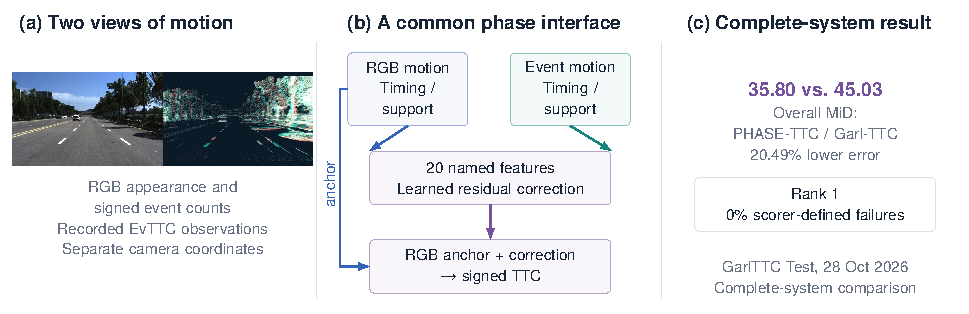
\includegraphics[width=\linewidth]{figures/publication_teaser.pdf}
\caption{\textbf{Estimate motion separately; combine it through phase.} (a) Recorded EvTTC RGB and event observations \citep{evttc}. (b) Each modality supplies phase, timing, and support features; a learned correction adjusts the RGB anchor. (c) The complete submitted system improves the archived GarlTTC Overall MiD score. The benchmark comparison does not isolate the contribution of any one component, and matched controls do not show a benefit from event access or from the phase parameterization.}
\label{fig:teaser}
\end{figure}
\clearpage
\section{Introduction}
As an object approaches a camera, its apparent size grows. For rigid frontal motion at approximately constant relative speed, the ratio of apparent size $s$ to expansion rate $\dot s$ gives time-to-contact (TTC), $T\simeq s/\dot s$. A recognizer can identify the object while leaving this rate undetermined; estimating when contact will occur requires recovering the change in scale. Rotation, occlusion, and camera motion complicate that measurement because they can alter the image independently of closing distance.

RGB frames provide texture and spatial context, while event cameras report asynchronous brightness changes along moving contours between frames \citep{eventsurvey}. To exploit both, a fusion method must account for the timing and support of each observation as well as the different representations learned from the two streams. We address this problem by estimating motion within each modality and combining quantities with shared meanings.

In PHASE-TTC, each branch supplies phase estimates together with timing and support information to a small residual network that adjusts an RGB anchor. The signed phase coordinate gives the branches a common description of approach and recession over a reference interval, allowing each to keep its own hidden representation. We preserve apparent expansion through common object coordinates and use temporal refiners to incorporate observations available before each query.

We evaluate PHASE-TTC as a complete TTC system, then examine its readout with matched controls. The private benchmark establishes system performance. To investigate the contribution of fusion, we hold the final upstream estimators and temporal histories fixed, compare simple combinations of their outputs, and train equally sized correction heads with or without event information. A separate local experiment asks whether learned routing adds value once apparent box expansion is available.

\subsection{Contributions}
We make three contributions:
\begin{enumerate}
\item \textbf{A causal phase-fusion architecture.} Independent motion estimators and temporal refiners supply a 20-field descriptor of phase, timing, and observation support to a 1,955-parameter residual head anchored on RGB. In the evaluated data most timing and support fields are constant, so the head acts mainly on ten phase values (Appendix~\ref{sec:physical-fusion-fields}). Table~\ref{tab:component-contracts} describes the nine-component system and its supervision.
\item \textbf{A benchmark result with matched readout controls.} The submitted system achieves \OfficialPhasePublishedOverallMiD{} Overall MiD on the archived GarlTTC Test leaderboard, against \OfficialGarlOverallMiD{} for the Garl-TTC reference. We complement this complete-system result with equal-capacity, equal-history head comparisons and simple fusion baselines on fixed final-model features. These controls do not show a benefit from event access or from the phase parameterization, so the benchmark gain is attributed to the complete system and not to the fusion interface (Sections~\ref{sec:official}--\ref{sec:design-analysis}).
\item \textbf{Geometric adaptation and runtime analysis.} We compare box expansion, fixed mixtures, and learned routing on the same queries to measure what each adds. A paced replay on a laptop GPU then measures numerical parity and end-to-end response against a 20\,ms deadline (Sections~\ref{sec:quality-adaptation}--\ref{sec:runtime}).
\end{enumerate}
The supplement retains the earlier predictive-learning, temporal, and physical-model investigations. They explain the design's development without serving as substitutes for the final-system comparisons.

\subsection{Relation to prior work}
\paragraph{Time-to-contact from apparent expansion.} The ratio of image size to its rate of change gives TTC without metric depth or speed \citep{lee1976}, and direct methods recover it from brightness derivatives for a planar surface \citep{horn2007}. Learned frame-based estimators regress or classify motion in depth between two images: optical expansion upgrades optical flow to scale change \citep{yang2020expansion}, Binary TTC decides whether contact occurs within a set of time thresholds \citep{badki2021bittc}, and scale-matching correlation searches explicitly across scales \citep{ling2023tpcv,ling2024scaleflowpp}. TSTTC provides a large frame-only driving benchmark for object-level TTC \citep{shi2023tsttc}. These methods use two frames; we do not evaluate against them, and their scale-aware matching is absent from our producers.

\paragraph{Event-based TTC and motion.} Event cameras support TTC through asynchronous flow \citep{clady2014}, contrast maximization with scaling or divergence models \citep{gallego2018cmax,mcleod2022}, and geometric fitting with spatio-temporal registration \citep{eventaided}. Dense event representations such as voxel grids and learned spike tensors feed convolutional backbones \citep{zhu2019voxel,gehrig2019est}, including correlation-based optical flow \citep{gehrig2021eraft}; event--frame fusion has reduced latency in automotive detection \citep{gehrig2024dagr}. EvTTC provides synchronized observations and a dedicated TTC benchmark \citep{evttc}; MVSEC and DSEC illustrate event--frame acquisition in driving conditions \citep{zhu2018mvsec,dsec}. The eAP study introduces geometry-aware representations, the logarithmic motion-in-depth metric, and early and late event--RGB fusion in the Garl models \citep{eap}. \paragraph{Position of this work.} Our contribution is the particular estimator interface: named motion estimates, timing, and support drive a residual correction around RGB. The phase coordinate itself comes from the benchmark geometry. Relative to feature-level late fusion, the interface exposes the meanings of its inputs and allows separate producer fitting. The matched tests below measure the utility of this readout under fixed producers; a matched hidden-feature fusion comparison is still needed to establish superiority over that alternative.

I-JEPA predicts target representations from context \citep{ijepa}, while VICReg regularizes representation variance and covariance \citep{vicreg}. These methods motivate our predictive-learning controls. Work on slow features shows that predictable distractors can dominate a learned state \citep{slowfeatures}; our experiments test how nuisance dynamics affect the information available for TTC. They support conclusions about the tested objectives and settings rather than a general impossibility of predictive learning.

\section{PHASE-TTC: independent estimates, shared phase}
\label{sec:train40}

\subsection{Deployed model composition}

PHASE-TTC deploys a causal chain of nine fitted components comprising four modality-specific producers, two pairwise temporal heads, two context refiners, and one fusion head. RGB and events each use a transport-trained baseline producer (A5) and a coarse-to-fine producer (C2F). The pairwise readouts extract phase features from their A5 representations, after which the context refiners incorporate temporal history. The fusion head anchors its correction on the refined RGB estimate. Figure~\ref{fig:deployed-architecture} traces this path; the five auxiliary rotations serve training only. \evidence{M22,M23}

\begin{figure}[htbp]
  \centering
  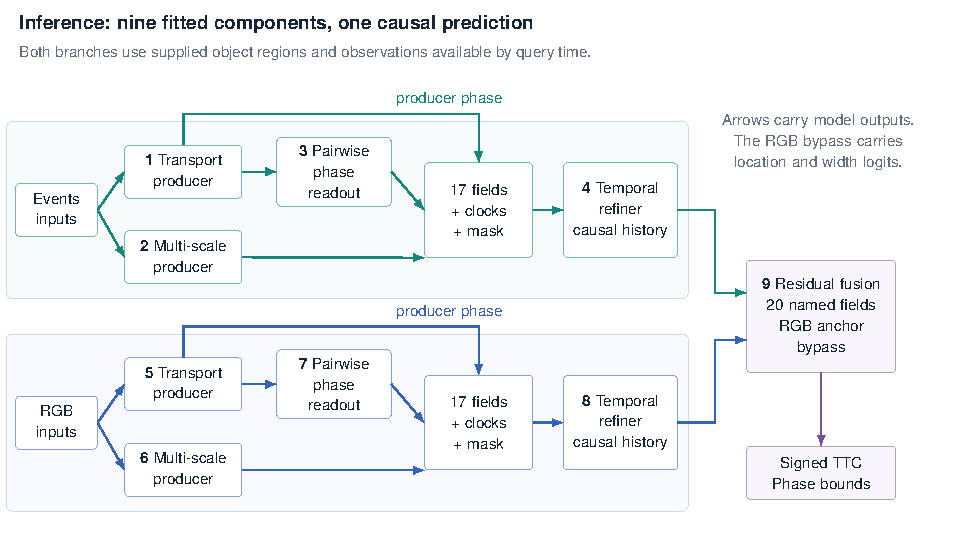
\includegraphics[width=\linewidth]{figures/publication_architecture.pdf}
  \caption{\textbf{Causal nine-component inference graph.} Supplied object regions feed parallel RGB and event producers, pairwise temporal heads, and temporal refiners. Twenty named fields enter the final RGB-anchored fusion head. \evidence{M03,M22,M23}}
  \label{fig:deployed-architecture}
\end{figure}

\begin{table}[htbp]
\centering\scriptsize
\caption{The nine fitted components in the submitted inference chain. RGB and event branches share the listed functional roles but have separate fitted weights. All targets and privileged supervision belong to fitting; inference uses sensor observations and supplied object regions.}
\label{tab:component-contracts}
\begin{tabularx}{\linewidth}{@{}p{.15\linewidth}p{.23\linewidth}p{.26\linewidth}X@{}}
\toprule
Components & Inputs & Architecture and outputs & Fitting signal \\
\midrule
Two transport producers & Shared-region temporal crops; observed endpoint intervals & Convolutional endpoint encoder, local feature correlation and scale residual; dense features, geometry and TTC & TTC, foreground/box geometry and RGB-derived relational distillation \\
Two coarse-to-fine producers & Same modality-specific crop contract & Two-scale local transport with a learned gate; alternate motion estimate & Producer objective with geometric and relational supervision \\
Two pairwise readouts & 133 fields derived from each transport producer's endpoints & LayerNorm, width-128 GELU MLP and scalar phase output & Smooth-L1 phase regression \\
Two context refiners & 17 fields per observation, four timing fields and validity mask & Two-layer width-160 GRU; phase correction around current expert median and phase widths & Group-weighted phase error, quantile losses and expert-relative costs \\
One fusion head & Ten named fields per modality; RGB anchor and width logits & Two width-32 layers with LayerNorm/SiLU; location and width corrections & Group-weighted phase error and quantile losses on out-of-fold features \\
\bottomrule
\end{tabularx}
\end{table}


\subsection{Object coordinates and causal history}

Each query includes supplied object coordinates. A common spatial frame covers both endpoint regions and preserves apparent scale change, which independent tight crops can erase. The evaluated system therefore assumes external localization.

Both branches use observations available by query time \(t\), with up to 650\,ms of causal history. Runtime begins at its declared measurement boundary and ends when the host receives the complete TTC output. Figure~\ref{fig:causal-history} separates the sensing interval from response time; its observation marks are schematic. \evidence{M03,M22,L43,L44}

\begin{figure}[H]
  \centering
  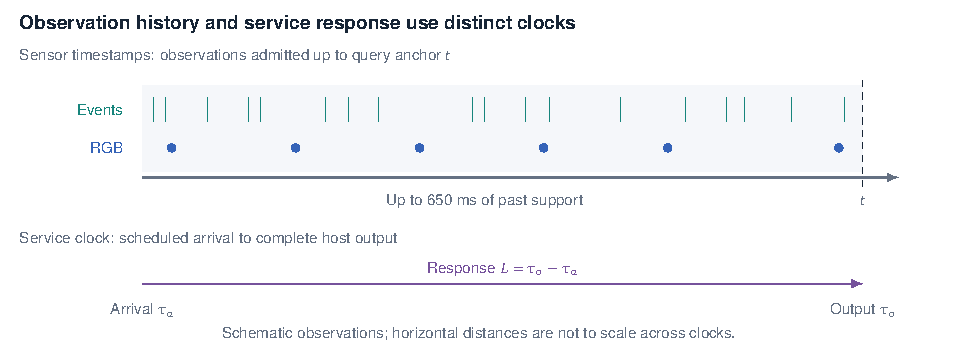
\includegraphics[width=\linewidth]{figures/publication_history.pdf}
  \caption{\textbf{Causal support and response-time boundaries.} RGB and event observations precede the sensor-time query anchor \(t\). A separate service clock measures from scheduled arrival \(\tau_a\) to complete host output \(\tau_o\); the two axes are schematic.}
  \label{fig:causal-history}
\end{figure}

\subsection{Phase as a shared motion coordinate}
Let $T$ denote signed TTC, positive for approach and negative for recession. With reference interval $d_0=0.1\,\mathrm{s}$, we use
\begin{equation}
 \phi(T)=-\log(1-d_0/T),\qquad T<0\ \text{or}\ T>d_0.
 \label{eq:phase-main}
\end{equation}
For large $|T|$, $\phi(T)\simeq d_0/T$: slow approach and recession lie near zero. Sensitivity increases toward the positive domain boundary $T=d_0$. This is a shared signed coordinate, not a removal of the near-contact singularity. The benchmark evaluates error in this coordinate; Section~\ref{sec:protocol} defines its weighting.

\subsection{A residual correction around RGB}
Each modality $m\in\{R,E\}$ exposes a vector $\mathbf{x}_m\in\mathbb{R}^{10}$: a raw phase location, the emitted point phase, three expert phases, four timing fields, and a valid-history count normalized by eight. The hidden state stays within its own branch. Let $D=\operatorname{diag}(\alpha^{-1}I_5,I_5)$, with $\alpha=0.03$. The fusion input is
\begin{equation}
 \mathbf{z}=[D\mathbf{x}_R;D\mathbf{x}_E]\in\mathbb{R}^{20}.
\end{equation}
Thus corresponding coordinates have the same meaning across modalities, while timing and support keep their native scaling. Appendix~\ref{sec:physical-fusion-fields} defines the timing fields precisely.

The residual network $g_\theta:\mathbb{R}^{20}\to\mathbb{R}^{3}$ uses two width-32 layers with LayerNorm \citep{ba2016} and SiLU activations:
\begin{equation}
 \mathbf c=g_\theta(\mathbf z).
\end{equation}
Its 1,955 parameters include the affine maps and both LayerNorms. Given the RGB raw-location anchor $\ell_R$ and width logits $\mathbf w_R$, the corrected location and widths are
\begin{align}
 \ell_F&=\ell_R+\alpha c_0,\\
 [\sigma_l,\sigma_u]^\top&=\alpha\operatorname{softplus}(\mathbf w_R+[c_1,c_2]^\top).
\end{align}
Zero initialization of the final affine layer's weights and bias starts optimization at the RGB anchor. The factor $\alpha$ scales the residual; it imposes no bound on $c_0$. The widths parameterize phase-interval endpoints and require empirical calibration before a probabilistic interpretation.

For a finite emitted prediction, we first clamp $\ell_F$ to $[\phi_{\min},\phi_{\max}]$, where $\phi_{\min}=-\log 2+10^{-6}$ and $\phi_{\max}=8$, then compute
\begin{equation}
 q_F=\frac{1-\exp(-\operatorname{clip}(\ell_F,\phi_{\min},\phi_{\max}))}{d_0},
 \qquad \widehat T=\frac{\operatorname{sgn}_{+}(q_F)}{\max(|q_F|,1/60\,\mathrm{s}^{-1})}.
\end{equation}
Here $\operatorname{sgn}_{+}(0)=1$, so zero phase emits $+60\,\mathrm{s}$. The rate floor limits the magnitude of emitted TTC near zero expansion. Figure~\ref{fig:fusion-interface} shows the anchor and correction paths; Appendix~\ref{app:implementation} gives the exact array layout, stable numerical inverse, and interval bounds. \evidence{M22,R02}

\begin{figure}[htbp]
\centering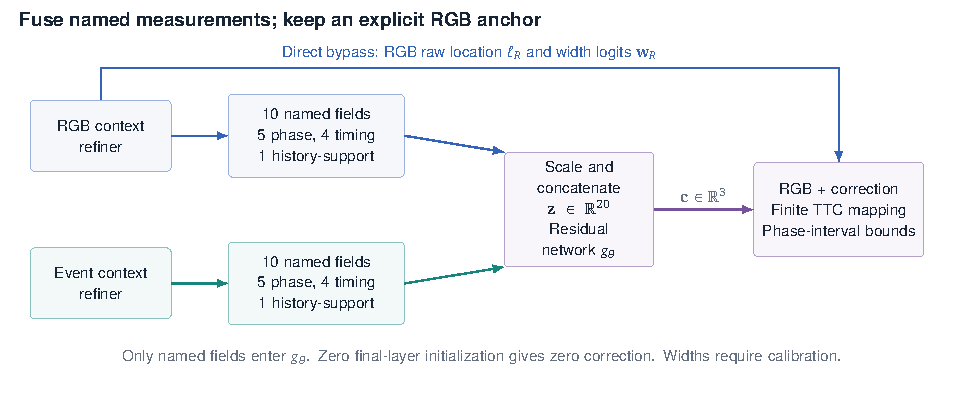
\includegraphics[width=\linewidth]{figures/publication_fusion.pdf}
\caption{\textbf{Shared measurements and an RGB anchor.} The two ten-field descriptors feed the residual network. RGB location and width logits also reach the output directly; only the learned correction passes through the network. Hidden features do not enter the fusion input.}
\label{fig:fusion-interface}
\end{figure}

\subsection{Submission coverage and benchmark status}

The official submission contains finite predictions without fallback for 6,762 query tokens across twelve sequences: 5,805 physical queries and 957 aliases. Aliases identify repeated physical queries and do not represent additional inference work.

Section~\ref{sec:official} reports the test result for this graph. Section~\ref{sec:design-analysis} holds the final upstream features fixed and refits matched correction heads to test their use of event information. \evidence{L44,B01,B02}

\FloatBarrier
\section{Training and evaluation}
\label{sec:protocol}

\subsection{Grouped out-of-fold training and final refitting}

Five rotations of eight-sequence blocks generate leakage-controlled inputs for the upper stages. In each rotation, twenty-four groups fit the four producers and two pairwise temporal heads, eight different groups fit the context refiners and normalizers, and the remaining eight groups generate out-of-fold features. A query group never contributes to supervised fitting of the models that generate its upper-stage features.

Within each auxiliary rotation, the context refiners fitted on its eight context groups generate twenty-field fusion features for its eight held-out groups. These fold-local feature sets are pooled to train the final fusion head. Separately, pooled seventeen-field RGB and event context inputs train the context refiners and normalizers used in the deployed forty-sequence chain; these final context models do not generate the fusion head's training inputs. Final pairwise temporal heads use representations from their corresponding forty-sequence transport-trained producers, so the out-of-fold claim applies to the specified context and fusion interfaces rather than every PAIR fit. \evidence{M23,P01}

We pool only named quantities whose meanings agree across rotations. Targets are joined after held-out feature generation. The two sets of pooled features fit different stages: context inputs fit the deployment refiners, while fold-local refined outputs fit fusion. Figure~\ref{fig:oof} separates these paths. Appendix~\ref{app:implementation} specifies their exact storage layout. \evidence{M22,M23,P01}

\begin{figure}[htbp]
\centering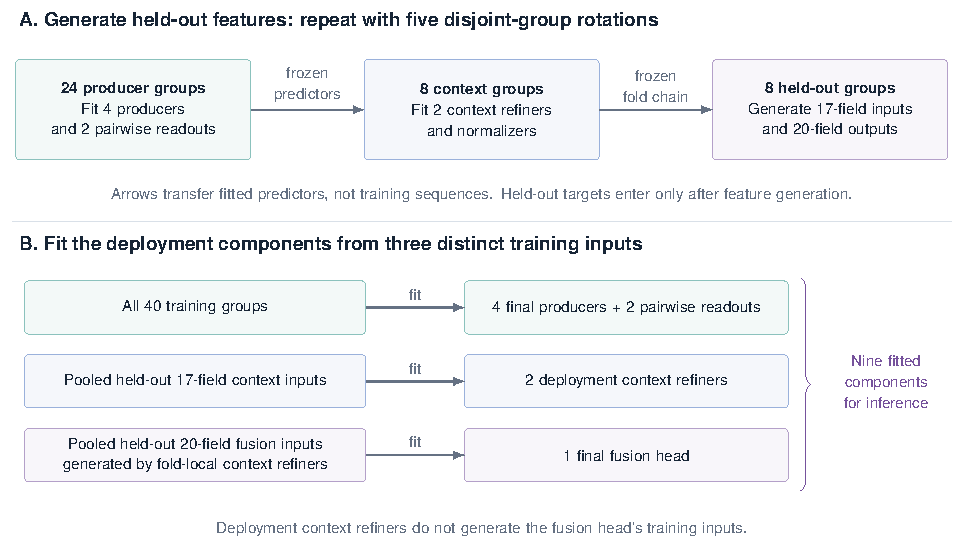
\includegraphics[width=\linewidth]{figures/publication_oof.pdf}
\caption{\textbf{Five-rotation fitting scheme.} Each rotation separates producer fitting, context fitting, and held-out feature generation. Final refitting produces one forty-sequence inference chain. \evidence{M23}}
\label{fig:oof}
\end{figure}

This grouped stacking procedure \citep{wolpert1992} separates feature generation from supervised fitting at each stage. Deployment uses one chain comprising four producers, two pairwise temporal heads, two context refiners, and the fusion head, with producers refitted on all forty groups. Auxiliary producer fits use twenty-four groups per rotation. The resulting change in producer-training population and prior architecture-selection exposure are considered when interpreting development results. Groups are complete sequences. The public metadata share one camera calibration across recordings and carry no session or location fields, so independence between sequences at the level of scene or acquisition session is an unverified assumption, both within the forty training sequences and between them and the twelve test sequences.

Producer training combines relational DINO teacher signals, foreground geometry supervision, and task-specific adaptation. The deployed chain no longer evaluates the generic teacher, but its supervision remains part of the training recipe. \evidence{L45}


\subsection{Metrics and target coordinates}
TTC error in seconds, inverse-TTC error, benchmark phase error, and detection of urgent risk measure different aspects of behaviour. We evaluate phase using Equation~\ref{eq:phase-main}. Negative TTC denotes recession. The interval $[0,0.1]$\,s is outside this transform's domain. The official benchmark scorer defines motion-in-depth (MiD) error as
\begin{equation}
 \mathrm{MiD}(\widehat T,T)=10^4\left|\log\left(1-\frac{0.1}{T}\right)
 -\log\left(1-\frac{0.1}{\widehat T}\right)\right|
 =10^4|\phi(\widehat T)-\phi(T)|.
\end{equation}
MiD measures phase displacement. At large positive $T$, the first-order approximation $\phi(T)\simeq0.1/T$ compresses differences in seconds, while sensitivity rises near the positive domain boundary. MAE in seconds complements MiD by retaining the physical time scale. \evidence{M10,M15}

The scorer groups target TTC into four right-closed intervals: crucial $c:(0,3]$\,s, small $s:(3,6]$\,s, large $l:(6,10]$\,s, and negative $n:(-10,0]$\,s. The grouping includes zero in the negative band, although the phase transform is undefined at zero; metric validity is checked separately. Targets outside these bands do not contribute to the band-weighted score.

The scorer computes the band-weighted score
\begin{equation}
 \mathrm{overall\_MiD}=0.5\,\mathrm{MiD}_{c}+0.3\,\mathrm{MiD}_{s}
                     +0.1\,\mathrm{MiD}_{l}+0.1\,\mathrm{MiD}_{n},
\end{equation}
and a sample-weighted mean MiD. Missing bands remain missing, without weight redistribution. The complete band-weighted score requires targets in all four bands. The source archive fixes the scorer version and includes checks of exact, imperfect, and missing-band cases. \evidence{M15}

Metric reductions retain failures explicitly. The wrapper records invalid predictions by band and leaves its strict mean unavailable when any row is invalid. The official failure rate differs from the false-negative rate for urgent collision warnings. Prediction coverage, invalid-MiD count, and risk recall accompany the corresponding error metrics. A finite saturated TTC may still carry an unsupported-measurement flag.

\subsection{Official benchmark and exploratory evaluations}

\begin{table}[H]
\centering\small
\caption{Evaluation populations and the quantities each supports. Historical46 and Extended-new share three sequence groups but no query identities. The 434-query inference snapshot and corrected local comparison share identities but answer different questions.}
\label{tab:evaluation-populations}
\begin{tabularx}{\linewidth}{@{}>{\raggedright\arraybackslash}p{.24\linewidth}>{\raggedright\arraybackslash}p{.22\linewidth}X@{}}
\toprule Population & Size & Interpretation \\\midrule
Official GarlTTC Test & 6,762 scored tokens & Private targets; band-weighted MiD and scorer-defined failures. \evidence{B01,B02} \\
Published Garl EvTTC & 3 sequences & Published RTE; target/query correspondence to this run unverified. \evidence{T02} \\
EvTTC competition snapshot & 434 queries; 10 sequences & Original 28 October predictions, coverage and disagreement; targets not verified at that snapshot. \evidence{T01} \\
Corrected local EvTTC & Same 434 queries & Original versus adapted PHASE-TTC error; historically exposed, local scoring, Slider-750 official equivalence unresolved. \evidence{N01} \\
Historical EvTTC transfer & 468 targets; 32 sequences & Original target assignment, superseded for Extended-new. Historical46 is unaffected by the correction. \evidence{L01,GT01} \\
EvTTC Historical46 & 46 targets; 3 sequences & Original target assignment, superseded for Extended-new. Historical46 is unaffected by the correction. \evidence{L01,GT01} \\
Corrected EvTTC transfer & 460 targets; 32 sequences & All 508 fixed candidates reassociated; development-exposed, supplied ROI. \evidence{GT01,GT02} \\
Cadence development & 2,608 queries; 25 recordings & Recording-macro paired comparison; 24 road recordings and Slider-500; historically exposed. \evidence{N02} \\
Native eAP replay & 5,805 physical queries; 6,762 template tokens & Local output sensitivity and coverage; private Test12 targets not scored for the candidate. \evidence{N03} \\
\bottomrule\end{tabularx}
\end{table}


The official GarlTTC Test submission covers twelve sequences and uses forty-sequence event--RGB inputs with up to 650\,ms of causal history. Section~\ref{sec:official} reports the public ranking as of 28 October 2026 over \OfficialSampleCount{} scored tokens, including aliases of repeated physical queries \citep{codabench2026}. The evaluator scores submitted TTC values without standardizing temporal support, localization, supervision, or runtime across systems. Separate development experiments probe mechanisms within their tested configurations. \evidence{B01,B02,L44}

\subsection{Local targets, scoring, and development reuse}
For local adaptation on EvTTC, we evaluate 434 corrected query correspondences across ten sequences using query-weighted MAE and mean relative error. We score the signed predictions and, separately, apply the organizer-described offline interpolation of negative predictions between valid outputs to both models. Their archived outputs contain two and one negative values, respectively. Interpolation may use later valid predictions and belongs only to offline scoring. Section~\ref{sec:quality-adaptation} reports the paired results and the sequence-specific scoring discrepancy. \evidence{N01}


The final quality-router fit excludes the ten evaluation recordings from its optimizer updates, but those recordings informed earlier design choices. The 460-query head comparisons likewise reuse inspected EvTTC recordings, while fitting only on source-domain eAP features. We interpret both as development evidence. Appendix~\ref{sec:canonical-cadence} retains the separate cadence and downstream selection experiments.

\subsection{Independence and paired comparisons}
Splits and resampling units are specified separately for each experiment; intervals use the percentile bootstrap \citep{efron1979}. Historical V5--V7 intervals resample sequence--track clusters; later studies use complete sequence groups, a sequence-to-track hierarchy, or scenario families. A sample-weighted sequence bootstrap carries all rows from each sampled group into the replicate and recomputes the ratio of summed losses to summed counts; sequence-macro summaries weight groups equally. A sequence-macro point estimate does not imply that its archived interval used sequence-level resampling. All reductions inherit any development exposure. Appendix~\ref{app:evaluation-details} identifies the study-specific units and gives the lineage, causality, and latency checks. \evidence{M15--M20,P02}

Three head seeds quantify optimization variability conditional on their parents; they do not independently replicate the upstream representation. The additional transfer bootstrap is post hoc: it resamples saved paired predictions without changing a model, split, or historical interval (Appendix~\ref{app:derived-transfer}).

For the new matched readout and geometry studies, 10,000 complete-recording resamples use seed 20261111. We fixed the model variants, training schedules, baseline mixture weights, and metric aggregation before running the comparisons, so their evaluation results could not guide these choices. These retrospective studies use the development-inspected recordings described above.

\subsection{Extent of development reuse}
The reported comparisons follow a long sequence of fits on the same recordings. The nine-sequence early development set was reused across the V5--V8 studies and the later temporal-context searches, the held-out H and V partitions across the V14--V19 studies, and the EvTTC adaptation population across at least 498 head, router, and adapter fits (21, 117, 312, and 48 in the campaigns of Appendices~\ref{app:adaptation-lineage} and~\ref{sec:canonical-cadence}). No correction for this multiplicity is applied to any interval in this article. Intervals on development recordings therefore describe the inspected cohort and understate the uncertainty of a new acquisition; only the private benchmark score is free of this exposure, subject to the submission caveats in Section~\ref{sec:official}.
\FloatBarrier

\FloatBarrier
\section{Three official submissions and what they measure}
\label{sec:official}

\subsection{Private-test results}

Table~\ref{tab:official-submissions} places the three PHASE-TTC submissions beside the documented Garl-TTC reference. Lower MiD is better. The original event--RGB system obtained 35.80 Overall MiD on 28 October 2026. A pre-registered RGB-plus-box-history submission obtained 23.47 on 18 November after removing event inputs. A third, pre-registered comparator on 21 November removed the RGB estimates as well and read only 600\,ms of supplied-box history; it obtained 27.98. All three scoring archives contain the same 6,762 tokens and zero scorer-defined failures. The downloaded third record, including its four band scores, is preserved in repository commit \texttt{8fa8dda6}. Because the public leaderboard retains one row per participant, dated submission records rather than a current leaderboard row preserve the three results.

\begin{table}[htbp]
\centering\footnotesize
\begin{tabularx}{\linewidth}{@{}p{.17\linewidth}p{.12\linewidth}p{.17\linewidth}Xp{.085\linewidth}p{.07\linewidth}@{}}
\toprule
Entry and date & Submission & Sensor inputs & Supplied-region and temporal support & Overall MiD & Failure \\
\midrule
Garl-TTC reference\\28 Jun 2026 & 817519 & Events + RGB & Supplied regions; two observations 0.1 s apart & 45.03 & 0\% \\
PHASE-TTC original\\28 Oct 2026 & 1016512 & Events + RGB & Supplied regions; up to 650 ms causal history & 35.80 & 0\% \\
PHASE-TTC-Geo\\18 Nov 2026 & 1058935 & RGB; no event input & Supplied regions; 600 ms box history within the 650 ms budget & 23.47 & 0\% \\
\bottomrule
\end{tabularx}

\caption{Official GarlTTC Test results over 6,762 tokens. ``Failure'' is the scorer-defined invalid-output rate, not a safety failure rate. The reference and PHASE systems use different models and temporal support.}
\label{tab:official-submissions}
\end{table}

The 23.47 result is 34\% below the original system and 48\% below the reference. The matched box-only comparator is 4.50325 MiD points higher than 23.47238; equivalently, adding the RGB estimates reduces Overall MiD by 16.10\% relative to the 27.97563 comparator. These official rows establish that supplied-region history alone is strong but does not reproduce the RGB-plus-geometry score under the tested recipes. They do not isolate a sensor-level causal effect or establish that supplied boxes replace event measurements under delayed or noisy detections, frame-filling objects, or another acquisition protocol.

\subsection{Metric and band asymmetry}

The scorer maps TTC to phase and reports
\begin{equation}
 \mathrm{MiD}(\widehat T,T)=10^4\left|\log\left(1-\frac{0.1}{T}\right)
 -\log\left(1-\frac{0.1}{\widehat T}\right)\right|.
\end{equation}
It then weights the crucial, small, large, and negative TTC bands by 0.5, 0.3, 0.1, and 0.1. The metric therefore emphasizes approaching contacts below 6\,s and is more sensitive near its positive-domain boundary. It is not an error in seconds. The second submission reduces the crucial-band score from 43.52 to 24.37; that 19.15-point change contributes 9.58 of the 12.33 Overall points. Changes in the small, large, and negative bands contribute 1.29, 0.28, and 1.18 points. The weighted result should not be summarized as a uniform improvement across TTC regimes.

\begin{table}[htbp]
\centering\small
\begin{tabular}{lrrrrr}
\toprule
Entry & Overall & Crucial & Small & Large & Negative \\
\midrule
Garl-TTC reference & 45.03 & 53.13 & 37.58 & 40.61 & 31.29 \\
PHASE-TTC original & 35.80 & 43.52 & 28.26 & 25.72 & 29.93 \\
PHASE-TTC-Geo & \textbf{23.47} & 24.37 & 23.95 & 22.89 & 18.13 \\
Box-history comparator & 27.98 & 26.39 & 28.00 & 32.94 & 30.89 \\
\bottomrule
\end{tabular}
\caption{Official band scores. Overall uses the 0.5/0.3/0.1/0.1 band weights rather than a sample-weighted mean.}
\label{tab:official-submission-bands}
\end{table}

The 6,762 tokens represent 5,805 physical queries and 957 aliases. Aliases reuse predictions at the same sensor query. The scorer flags nonfinite TTC or $|\widehat T|<0.1$\,s as failures, then averages finite MiD values by band. Zero scorer-defined failures therefore certifies finite admissible outputs under that rule; it does not certify calibrated risk, localization, or safe operation.

\subsection{Comparator and modality boundaries}

The official reference row comes from the leaderboard and was not reproduced locally for Table~\ref{tab:official-submissions}. Garl-TTC and the original PHASE-TTC both use events, RGB, and supplied regions, but Garl-TTC estimates a height ratio from two observations 0.1\,s apart while PHASE-TTC aggregates up to 650\,ms of branch history. The benchmark does not standardize temporal support, training data, learned components, or runtime. The 35.80-versus-45.03 difference belongs to the complete systems.

Separate local controls use the released Garl checkpoints under their native input contract. They select the latest causal RGB endpoint and the preceding endpoint nearest 100\,ms, construct a polarity-agnostic 20-plane event time volume at each endpoint with at most 100\,ms support, and use the supplied regions to form a common square crop. The adapter substitutes the measured endpoint separation in the height-ratio-to-TTC conversion; it does not refit the checkpoint. Full, event-only, and visual-only routes have different input availability, and these development-exposed runs are not the official leaderboard comparison (Appendix~\ref{app:competition-details}). In the later service experiment, a CPU path constructs Garl event volumes on cache misses and hashes prepared inputs inside the measured call. Its timing is specific to that implementation and is not a lower bound for Garl-TTC.

The geometry submission changes both modality and measurement access. It uses no event input, but it receives 600\,ms of causal box expansion in addition to RGB-branch estimates. The leaderboard fact sheet displays its ``Uses Event'' field as empty rather than false. We retain that downloaded record and derive the no-event statement from the bound recipe and scored package, not from the empty form field. The third submission uses the same supplied-box history and a learned geometry head but no RGB image estimates and no event input. It is an official matched comparator, not a replacement release for PHASE-TTC-Geo.

\subsection{Selection, exposure, and attribution}

The original system was the author's first test submission. The geometry variant was chosen by a rule fixed on TRAIN40 development folds and then submitted once with a receipt that bound its code, seed, package, and hypothesis. Those folds showed 85.17 Overall MiD for the released recipe and 41.27 for the selected geometry head, but fold and server levels differ enough that these values must not be pooled or used as a calibration curve. The private result confirms the direction of the geometry intervention, not the size predicted by the folds. The box-only comparator was likewise bound before its third upload and was reported whether or not it beat 23.47. Its 27.98 score provides a private-test ablation of RGB estimates conditional on the fitted heads and shared box-history contract.

Only the three private-test scores use targets that the project did not inspect during development. They are sequential exposures to the same server, not independent test sets: the earlier score was known before each later recipe was uploaded. Transfer, routing, event-history, literature-baseline, and FCWD controls reuse inspected recordings or open labels. They identify failure modes and plausible mechanisms without providing another independent test. Appendix~\ref{sec:post-audit-geometry} records the second submission and its fold analysis; the third submission record and pre-registered matched-comparator protocol preserve the box-only comparison. Appendix~\ref{sec:followup} records later controls and their exposure.

\subsection{Original submission by band}

Table~\ref{tab:official-benchmark} retains the full-precision calculation for the original submission and the dated reference. Percentage reductions combine the unrounded PHASE-TTC scorer values with the reference's displayed two-decimal values.

\begin{table}[H]
\centering\small
\caption{Official GarlTTC Test scores on 28 October 2026 (lower is better). PHASE-TTC scores are shown to four decimals and Garl-TTC at published precision. Relative reductions use unrounded PHASE-TTC scores. Both entries have 6,762 scored tokens and 0\% scorer-defined failures. \evidence{B01,B02}}
\label{tab:official-benchmark}
\begin{tabular}{lrrr}
\toprule
\textbf{Metric} & \textbf{PHASE-TTC} & \textbf{Garl-TTC} & \textbf{Decrease} \\
\midrule
Overall & 35.8015 & 45.03 & 20.49\% \\
Crucial & 43.5190 & 53.13 & 18.09\% \\
Small & 28.2568 & 37.58 & 24.81\% \\
Large & 25.7179 & 40.61 & 36.67\% \\
Negative & 29.9314 & 31.29 & 4.34\% \\
\bottomrule
\end{tabular}
\end{table}


For band $b$, the additive contribution to the original-versus-reference difference is $w_b(\mathrm{MiD}^{\mathrm{Garl}}_b-\mathrm{MiD}^{\mathrm{PHASE}}_b)$. The crucial and small bands contribute \OfficialCrucialSmallContributionShare{} of that Overall difference. This decomposition reflects the benchmark weights and must remain separate from sample-weighted mean MiD or TTC error in seconds.

The current platform does not regenerate the historical original predictions byte for byte. A native replay changes 504 of 5,805 physical-query TTC values beyond the historical tolerance. Converting the largest admissible displacement of each replayed output to the benchmark coordinate gives a mean bound of 0.010 MiD and a maximum of 0.30 for one query, without access to private targets. The scored package and its official result remain the evidence for 35.80; local repeatability does not replace them.
\FloatBarrier

\section{When does fusion improve on RGB?}
\label{sec:late-transfer}
\cohortline{CORRECTED TRANSFER / \AuditTransferCount{} eligible of 508 candidates / 32 development-exposed sequences / supplied ROI}

The frozen-modality comparison tests whether the shared phase interface improves errors in seconds beyond the benchmark setting. Fusion has lower point MAE and p95 than RGB alone on the revised cohort, whereas RGB retains lower median and relative error. Paired sequence-bootstrap intervals for mean, median, and p95 differences include zero, so the cohort does not resolve an ordering between the two.

\subsection{Evaluation population}
We evaluate frozen predictions on \AuditTransferCount{} eligible queries from 32 EvTTC sequences. The registered sampling contains 508 candidate queries; eligibility requires a public TTC label within 50\,ms of the query, with ties assigned to the earlier timestamp. All eligible targets are positive. The primary annotated object supplies the query region. These sequences had been used during development, as specified in Section~\ref{sec:protocol}.

A source audit identified a reversed low/medium target assignment for two recordings in our earlier analysis. Matching the public download identities and source hashes corrected this association without changing sensor queries or predictions. We report only the corrected cohort here; Appendix~\ref{app:target-association} records all candidate counts, exclusions, and the superseded assignment.

\subsection{Corrected error distribution}
Relative time error remains $100|\widehat T-T|/|T|$. Pooled summaries weight queries equally; sequence-macro summaries weight each sequence group equally. Temporal support differs across complete systems: PHASE-TTC uses up to 650\,ms of history, while Garl uses two observations separated by 0.1\,s.

\begin{table}[htbp]
\centering\small
\resizebox{\linewidth}{!}{%
\begin{tabular}{lrrrrrrr}
\toprule
Cohort / model & $n$ & MAE & Median & p95 & RTE (\%) & Macro MAE & Macro RTE (\%) \\
\midrule
Corrected extended: PHASE-TTC & 460 & 0.813 & 0.446 & 2.742 & 29.112 & 0.827 & 30.016 \\
Corrected extended: RGB context & 460 & 0.851 & 0.390 & 3.038 & 29.017 & 0.859 & 29.368 \\
Corrected extended: Event context & 460 & 1.376 & 0.844 & 3.707 & 58.154 & 1.377 & 57.764 \\
Corrected extended: Garl full & 460 & 3.166 & 0.635 & 4.781 & 131.268 & 3.041 & 126.366 \\
Historical46: PHASE-TTC & 46 & 0.141 & 0.136 & 0.250 & 7.748 & 0.159 & 8.419 \\
Historical46: RGB context & 46 & 0.113 & 0.099 & 0.264 & 6.387 & 0.114 & 6.246 \\
Historical46: Event context & 46 & 0.286 & 0.241 & 0.692 & 15.822 & 0.289 & 15.566 \\
Historical46: Garl full & 46 & 0.250 & 0.186 & 0.561 & 13.327 & 0.282 & 14.649 \\
\bottomrule
\end{tabular}
}
\caption{Corrected-label transfer: 460 eligible of 508 extended candidates across 32 sequences. Historical46 remains separate (46 queries, three sequences). Absolute errors are seconds; macro gives equal weight to sequences.}
\label{tab:audit-transfer-summary}
\end{table}


Fusion MAE is \AuditFusionMAE{}\,s against RGB's \AuditRgbMAE{}\,s; its empirical p95 is \AuditFusionPninetyfive{}\,s against \AuditRgbPninetyfive{}\,s. RGB retains lower median error, \AuditRgbMedian{} versus \AuditFusionMedian{}\,s, and slightly lower RTE, \AuditRgbRTE{} versus \AuditFusionRTE{}.  \evidence{GT01}



\subsection{Exceedance and paired uncertainty}
The full corrected distribution retains signed predictions, including large errors. Appendix~\ref{app:extra-diagnostics} shows the fraction at or above each absolute-error threshold. Maximum absolute error is \AuditFusionMax{}\,s for fusion and \AuditRgbMax{}\,s for RGB. These are query-level errors under the corrected labels, not scorer-defined invalid predictions.



The PHASE-minus-RGB mean difference is \AuditMeanDelta{}\,s with interval $[\AuditMeanLow,\AuditMeanHigh]$\,s; the p95 difference is \AuditPninetyfiveDelta{}\,s with interval $[\AuditPninetyfiveLow,\AuditPninetyfiveHigh]$\,s. All three paired intervals include zero. The procedure uses 10,000 complete-sequence resamples with linear quantiles and the same frozen models.

Two observations show how fragile the ordering of means is. Under the superseded target assignment, RGB had the lower MAE by 0.007\,s; correcting the targets of two recordings moved the difference to \AuditMeanDelta{}\,s in favor of fusion without changing any prediction. On the earlier 46-query subset, RGB is better in mean and median with intervals that exclude zero (Table~\ref{tab:audit-transfer-bootstrap}). We therefore do not claim that fusion improves on RGB in seconds on EvTTC.

Eligibility removes 48 candidates whose query lies between 54 and 2,055\,ms from the nearest public label; each sits at the edge of its recording's labeled span, where the nearest label has a median TTC of 2.2\,s. The rule is independent of every prediction and identical for all models, and every excluded candidate has finite predictions from all four systems. Appendix~\ref{app:derived-transfer} gives complete sequence results and distinguishes this corrected analysis from the historical one.
\begin{table}[htbp]
\centering\small
\resizebox{\linewidth}{!}{%
\begin{tabular}{lllrr}
\toprule
Cohort & Paired contrast & Estimand & Difference & 95\% interval \\
\midrule
Extended460 & PHASE minus RGB & mean & -0.038 & [-0.147, +0.061] \\
Extended460 & PHASE minus RGB & median & +0.055 & [-0.042, +0.136] \\
Extended460 & PHASE minus RGB & p95 & -0.296 & [-0.657, +0.193] \\
Extended460 & PHASE minus Garl & Macro MAE\_s & -2.214 & [-4.951, -0.447] \\
Extended460 & PHASE minus Garl & Macro RTE\_pct & -96.350 & [-211.946, -16.629] \\
Historical46 & PHASE minus RGB & mean & +0.028 & [+0.005, +0.103] \\
Historical46 & PHASE minus RGB & median & +0.036 & [+0.026, +0.068] \\
Historical46 & PHASE minus RGB & p95 & -0.014 & [-0.098, +0.109] \\
Historical46 & PHASE minus Garl & Macro MAE\_s & -0.123 & [-0.178, -0.084] \\
Historical46 & PHASE minus Garl & Macro RTE\_pct & -6.230 & [-8.682, -4.767] \\
\bottomrule
\end{tabular}
}
\caption{Whole-sequence paired percentile intervals. PHASE--RGB uses 10,000 draws, seed 20261028, for pooled query errors; PHASE--Garl uses 2,000 draws, seed 7, for equal-sequence means. Linear quantiles; negative favors PHASE. MAE, median and p95 use seconds; RTE uses percentage points. Exposed development cohorts.}
\label{tab:audit-transfer-bootstrap}
\end{table}

\FloatBarrier

\section{Matched tests of the final fusion readout}
\label{sec:design-analysis}
The official result compares complete systems. Here we isolate readout choices while holding the final RGB and event producers, temporal refiners, supplied regions, and causal histories fixed. We use the same 460 corrected transfer queries throughout. These recordings informed earlier development; the new comparisons quantify conditional effects on that cohort.

\subsection{Simple combinations of identical branch outputs}
We first replace the released fusion head with equal mixtures of the two final branch predictions, combining them in phase, inverse TTC, or seconds. Each mixture receives the same branch outputs and temporal support. All emit finite TTC under their specified numerical policies. Table~\ref{tab:revision-fixed} shows that learned fusion improves mean error over these fixed combinations. Its comparison with the strong RGB branch remains uncertain (Section~\ref{sec:late-transfer}); the equal mixtures are also worse than RGB alone, because the event branch is the weaker constituent.
\begin{table}[htbp]
\centering\small\begin{tabular}{lrrr}
\toprule
Frozen readout & MAE (s) & Median (s) & p95 (s) \\
\midrule
Released fusion & 0.813 & 0.446 & 2.742 \\
RGB context & 0.851 & 0.390 & 3.038 \\
Event context & 1.376 & 0.844 & 3.707 \\
Equal phase mixture & 0.997 & 0.519 & 2.759 \\
Equal inverse-TTC mixture & 1.007 & 0.518 & 2.762 \\
Equal TTC mixture & 1.050 & 0.614 & 3.192 \\
\bottomrule
\end{tabular}

\caption{Frozen final-branch readouts on the identical 460 queries. Equal mixtures have no fitted parameters; the released head has 1,955. This comparison holds upstream information fixed but does not match readout capacity.}
\label{tab:revision-fixed}
\end{table}

\subsection{Equal-capacity heads with matched fitting}
To distinguish event access from added correction capacity, we fit three heads: the original phase readout; an identical head whose ten event fields are zero during fitting and evaluation; and a residual readout expressed in inverse TTC. All contain 1,955 parameters, start with a zero final affine map, and retain the RGB anchor. The zero-event head still receives RGB timing and support. Upstream weights are frozen throughout.

Each arm uses the same 88,744 source-domain out-of-fold feature rows from forty eAP recordings, the same seeded minibatch sequence, and 12,044 AdamW \citep{loshchilov2019} updates at batch size 128. We retain the original warmup/cosine schedule, weight decay, clipping, and phase-error plus quantile objective. Seeds 7, 13, and 21 vary only the correction-head fit. EvTTC queries and targets are excluded from fitting and checkpoint selection; every arm uses its final update. The inverse-TTC arm replaces phase inputs with normalized rates and predicts an RGB rate correction before conversion to the common phase loss. Appendix~\ref{app:consolidation-reproduction} specifies the transforms and archived source bindings.

We also fit a single scalar phase-mixture weight on the source training rows alone. Searching the specified 101-point grid gives event weight 0.31. This is a train-calibrated simple baseline, evaluated once on EvTTC.
\begin{table}[htbp]
\centering\small\begin{tabular}{lrr}
\toprule
Readout & MAE (s) & Relative error (\%) \\
\midrule
Phase correction, real events & $0.847\pm0.038$ & $30.92\pm2.05$ \\
Phase correction, zero events & $0.838\pm0.021$ & $29.12\pm1.16$ \\
Inverse-TTC correction, real events & $0.847\pm0.041$ & $30.80\pm2.14$ \\
Source-calibrated scalar phase mixture & 0.996 & 36.23 \\
\bottomrule
\end{tabular}

\caption{Matched final-head fitting. Values are the mean and sample standard deviation of the three seed-level scores; predictions are not ensembled. The scalar mixture has one fitted coefficient and no seed-dependent optimization.}
\label{tab:revision-heads}
\end{table}

\subsection{What the controlled comparison establishes}
Real events improve MAE over the zero-event control for one seed and worsen it for two. The mean zero-minus-real difference is $-0.0094$\,s, with a descriptive recording-bootstrap interval spanning zero. Inverse-TTC and phase corrections are also indistinguishable at this resolution. The refitted phase heads are not distinguishable from the RGB anchor they correct: the RGB-minus-head difference is $+0.004$\,s with an interval from $-0.089$ to $+0.114$\,s, and the seed-13 head is worse than RGB alone. We average paired losses over the three fixed seeds before resampling complete recordings, preserving query correspondence; seeds do not multiply the number of independent recordings.
\begin{table}[htbp]
\centering\small\begin{tabular}{lrr}
\toprule
Paired contrast & $\Delta$MAE (s) & 95\% interval (s) \\
\midrule
Zero events minus real events & -0.0094 & $[-0.0780,+0.0630]$ \\
Inverse TTC minus phase & -0.0003 & $[-0.0061,+0.0058]$ \\
Calibrated mixture minus phase & +0.1492 & $[+0.0064,+0.3762]$ \\
Calibrated mixture minus phase, without CPNAO-high & +0.0564 & $[-0.0104,+0.1261]$ \\
RGB context minus phase & +0.0043 & $[-0.0886,+0.1140]$ \\
Released head minus refitted phase & -0.0340 & $[-0.0831,-0.0014]$ \\
\bottomrule
\end{tabular}

\caption{Paired differences after averaging query losses over fixed head seeds; 10,000 complete-recording resamples across 32 recordings, or 31 for the row without CPNAO-high. ``Phase'' denotes the three-seed refitted phase head with real events. These intervals describe the inspected cohort and condition on the shared upstream models.}
\label{tab:revision-paired}
\end{table}

The learned readouts improve on the calibrated scalar mixture, but that margin is concentrated in one recording: without CPNAO-high the difference falls from $+0.149$ to $+0.056$\,s and its interval, $[-0.010,+0.126]$\,s over 31 recordings, includes zero. The tests give no consistent incremental benefit from event access and no observed advantage of phase over the tested inverse-TTC parameterization. On this cohort the refitted heads are therefore best described as reproducing the RGB branch; the controls do not establish a useful correction, and they do not support attributing the benchmark gain to event--RGB fusion.

The released head has a lower MAE than the mean of its three refits, 0.813 against 0.847\,s, and the released-minus-refit interval, $[-0.083,-0.001]$\,s, excludes zero. The released head and the seed-7 refit, at 0.8135\,s, share that seed. Seed 7 was fixed before these EvTTC comparisons and was not chosen on them, but the released value is the most favorable of the three seeds on this cohort, and the three-seed mean is the better estimate of the recipe's transfer error.

These controls share one further limitation. The event branch receives evaluation inputs whose history cadence and support differ from those used to fit it (Appendix~\ref{sec:field-ranges}). A later control that rebuilds the event history on the training grid, with all models frozen, also finds no measurable benefit (Appendix~\ref{sec:post-audit-event-history}). These null results concern the deployed event path; they do not show that events are uninformative for TTC. The prior positive event control used a different adapted model; Appendix~\ref{app:design-history} preserves that result without transferring its attribution to the submitted system. A matched hidden-feature fusion model and genuinely unused recordings remain necessary to compare broader fusion designs.
\FloatBarrier

\section{Does learned routing add value beyond box geometry?}
\label{sec:quality-adaptation}
The geometric extension combines the frozen fused, RGB, and event estimates with apparent expansion from supplied box history. We fit inverse TTC from width, height, and square root of area over the preceding 650\,ms, using median pair slopes \citep{sen1968} and a query-time intercept. A 688-parameter gate uses fit quality and expert agreement to weight the four inverse-TTC estimates; the delivered adapter averages three independently seeded gate outputs in seconds. Its fit uses 2,608 queries from 24 road recordings and Slider-500. Ten of those road recordings are the 0\% and 50\% overlap siblings of five evaluated recordings (CCRm-low, CCRm-medium, and the three CCRs-1 speeds): distinct acquisitions of the same scenario and speed class. The three evaluated CCRs-2 recordings have no sibling in the fitting population. Appendix~\ref{app:quality-complete} gives the geometry, 33 input fields, training recipe, and fallback rules.

\subsection{Matched experts, timing, and coverage}
We compare the original model, geometry alone, geometry with original-model fallback, a fixed half-and-half inverse-TTC mixture, and the released router. All use the same saved causal inputs and 434 corrected target correspondences. The fixed weight is specified before calculating these comparisons. The fixed mixture combines two estimates, the original fusion and geometry, whereas the router weights four and receives 33 descriptors; a router-minus-mixture difference therefore includes access to the separate RGB and event estimates as well as learned routing. Geometry is available on 424 queries, including 357 of 365 road queries. Table~\ref{tab:revision-geometry} reports both available coverage and identical geometry-valid support; an abstention never silently changes a comparator's denominator. We retain signed outputs and the shared finite emission policy. Organizer-style interpolation appears only in the separate supplementary analysis.

\begin{table}[htbp]
\centering\small
\begin{tabular}{lrrrr}
\toprule
Estimator & Coverage & Available & Common & Road common \\
\midrule
Original fusion & 434/434 & 0.824 & 0.793 & 0.282 \\
Geometry only & 424/434 & 1.158 & 1.158 & 1.343 \\
Geometry with original fallback & 434/434 & 1.181 & 1.158 & 1.343 \\
Fixed inverse-TTC mixture & 434/434 & 0.333 & 0.289 & 0.221 \\
Learned router & 434/434 & 0.347 & 0.304 & 0.159 \\
\bottomrule
\end{tabular}

\caption{Matched adaptation errors in seconds. Available-support MAE uses the displayed coverage;
the common column uses the same 424 queries for every arm, and road common uses the same 357.
Predictions retain their signs.}
\label{tab:revision-geometry}
\end{table}


On common support, geometry alone has lower median error but large outliers, yielding mean error 1.158\,s. A fixed mixture reduces MAE to 0.289\,s, compared with the router's 0.304\,s; the fixed-minus-router paired MAE difference is $-0.0146$\,s, with a 95\% recording-bootstrap interval of $[-0.1704,0.0943]$\,s. On the pooled common support the fixed mixture therefore has the lower point error. The road-only comparison differs: across eight recordings and 357 queries, the router reduces MAE from the fixed mixture's 0.221 to 0.159\,s, with a fixed-minus-router difference of 0.062\,s and a recording-bootstrap interval of $[0.014,0.120]$\,s. Three recordings, CCRm-low, CCRm-medium, and CCRs2-low, supply most of that difference; the router is worse than the mixture on CCRs1-high (0.114 against 0.073\,s) and within 0.03\,s of it on the remaining four. A percentile interval over eight clusters is imprecise. Excluding Slider-750 also favors the router, by 0.057\,s with interval $[0.008,0.111]$\,s across nine recordings. These are descriptive comparisons on development-used data.

Thus adding geometry explains most of the improvement: on the road subset it accounts for 0.061 of the 0.123\,s reduction from the original model, and on the pooled support for all of it. Learned routing adds a further road-subset gain that depends on three recordings, two of which have sibling acquisitions in the router's fitting population, and that was observed on development-used data. We regard it as a hypothesis for independent data, not as an established benefit. The original model's locally reconstructed organizer-style score still disagrees for Slider-750. Appendix~\ref{par:local-score-correspondence} gives the exact discrepancy, without attributing it to an unverified physical cause. Independent recordings with detector-produced boxes are needed to test whether the routing benefit persists under new geometry errors.
\FloatBarrier

\section{Runtime and causal service}
\label{sec:runtime}

The deployment measurements in this article use persistent services: weights remain resident, state advances with causal sensor arrivals, and previously computed work is reused when its inputs are unchanged. PHASE and Garl receive the same paced RAW replay. The primary response clock begins at scheduled arrival and ends when the required TTC output is available on the host. It includes sensor release, scheduling and queueing, region preparation, neural computation, synchronization, and delivery. Model loading, synthetic shape priming, history initialization, and RAW disk preload occur before measured arrivals. This is a CPU-fed sensor replay, not a physical-camera measurement.

\begin{figure}[H]
\centering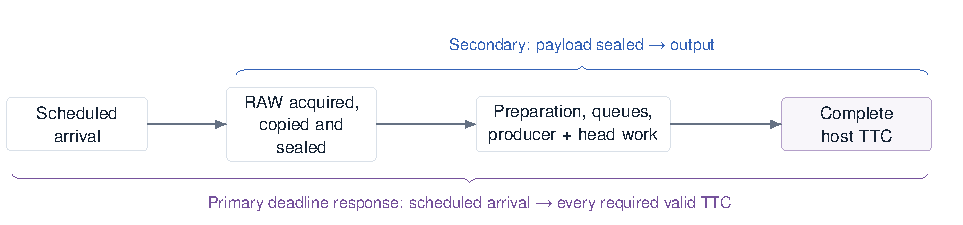
\includegraphics[width=\linewidth]{figures/publication_runtime_clock.pdf}
\caption{\textbf{Persistent-service response clocks.} The primary clock starts at scheduled arrival. The secondary clock starts after RAW acquisition, copy, and payload sealing. Both end at completed host TTC output. Service time starts only when the consumer begins work and is reported separately.}
\label{fig:runtime-clocks}
\end{figure}

\subsection{Persistent execution and exact reuse}

PHASE prepares RGB within the object region, extends event prefixes incrementally, and reuses reverse-transport summaries exactly. Top-$k$ normalization and native query graphs reduce repeated work; parallel branches overlap event execution with RGB preparation. Previously computed RGB producer features are reused under matching identities, while event encodings and temporal readouts are recomputed. Native numerical agreement is checked separately for the complete output chain. The complete nine-component model is retained.

The comparator is persistent TTC-only Garl. Its weights and causal event history remain resident; exact endpoint representations and the six-channel paired RGB backbone result are reused only under matching sensor, geometry, model, and preprocessing identities. Its event backbone and TTC heads execute on every completed update. Auxiliary foreground decoders are disabled because their masks do not feed the TTC output. All raw heights and TTC predictions are verified against untouched native inference after timing; the complete checkpoint remains loaded.

Compiled transport alternatives that changed PHASE's TTC on sensitive examples were rejected. An earlier smaller-packet experiment established numerical equivalence but did not establish paced-service latency. Neither result is substituted for the measured production-service response. \evidence{L41,L42}

\subsection{Expanded repeated inference study}

The subsequent campaign extends the comparison to six recorded car and pedestrian scenarios, using 1,979 distinct sensor-clock anchors and continuous intervals up to 9.3\,s. It retains 72 fresh-process attempts: four repetitions per model and scenario with queue capacity two, and two additional repetitions with queue capacity 64. All timing finishes before independent native-reference inference begins, and both services apply a fixed rest after initialization. This separates the expanded evidence from the initial experiment's interleaved reference workload.

\begin{table}[H]
\centering\small
\caption{\textbf{Expanded persistent-service comparison at 50\,Hz.} S1--S6 denote CPLA-low, CCRm-medium-0, CCRs-3-low-100, CCRs-side-high, CPNA-high and CPNAO-high. Q2 and Q64 denote queue capacities two and 64. D/A/N gives complete deliveries, numerically admitted runs and declared attempts. Median per-pass p95 (ms) requires full delivery and native parity in all four Q2 repetitions or both Q64 repetitions; all attempts remain in the full tables.}
\begin{tabular}{llrrrr}
\toprule
Scene & Model & Q2 D/A/N & Q2 p95 & Q64 D/A/N & Q64 p95 \\
\midrule
S1 & PHASE & 0/0/4 & --- & 2/2/2 & 121.66 \\
S1 & Garl & 0/0/4 & --- & 2/2/2 & 2932.78 \\
S2 & PHASE & 0/0/4 & --- & 2/0/2 & --- \\
S2 & Garl & 0/0/4 & --- & 2/2/2 & 1741.70 \\
S3 & PHASE & 1/1/4 & --- & 2/2/2 & 105.15 \\
S3 & Garl & 0/0/4 & --- & 0/0/2 & --- \\
S4 & PHASE & 0/0/4 & --- & 2/2/2 & 226.71 \\
S4 & Garl & 0/0/4 & --- & 0/0/2 & --- \\
S5 & PHASE & 0/0/4 & --- & 2/2/2 & 175.53 \\
S5 & Garl & 0/0/4 & --- & 2/2/2 & 4934.71 \\
S6 & PHASE & 0/0/4 & --- & 2/2/2 & 103.72 \\
S6 & Garl & 0/0/4 & --- & 1/1/2 & --- \\
\bottomrule
\end{tabular}

\end{table}

With the two-packet queue, PHASE completed 1/24 full replays and delivered 762/7,916 outputs (9.6\%). Of all offered updates, 178 (2.2\%) completed below 20\,ms. Strict native parity admitted 1/24 full replays; 0 delivered outputs failed at least one required numerical check.

With the two-packet queue, Garl completed 0/24 full replays and delivered 72/7,916 outputs (0.9\%). Of all offered updates, 0 (0.0\%) completed below 20\,ms. Strict native parity admitted 0/24 full replays; 0 delivered outputs failed at least one required numerical check.

With the 64-packet queue, PHASE completed 12/12 full replays and delivered 3,958/3,958 outputs (100.0\%). Of all offered updates, 1,217 (30.7\%) completed below 20\,ms. Strict native parity admitted 10/12 full replays; 6 delivered outputs failed at least one required numerical check.

With the 64-packet queue, Garl completed 7/12 full replays and delivered 3,816/3,958 outputs (96.4\%). Of all offered updates, 429 (10.8\%) completed below 20\,ms. Strict native parity admitted 7/12 full replays; 0 delivered outputs failed at least one required numerical check.

Appendix~\ref{sec:extended-inference} reports cohort selection, complete architecture and execution contracts, per-pass distributions, service and queue clocks, deadline coverage, buffered response traces, memory, startup, source age and independent numerical verification. A larger queue can preserve more packets while increasing the age of delivered TTC; those diagnostic results are kept separate from the two-packet primary policy.

Three cautions apply to this table. First, the Garl response times are not lower bounds for that method. Its median service time is shorter than PHASE's; its multi-second p95 values arise from a CPU event-volume construction on cache misses in our persistent-service implementation, which then backs up the queue. Second, under the two-packet policy almost every replay of either model ends after a few outputs. In 23 of the 24 PHASE passes the first service call takes 130--200\,ms, and about 95\,ms in every Garl pass, which fills the queue and triggers history-gap refusals for the remainder of the interval; in the one completed PHASE pass it takes 24\,ms. This campaign introduced a fixed 15\,s rest after initialization, after which the recorded GPU core clock has a median of 285\,MHz against 1,560\,MHz before it. The completed pass followed the same rest, so the rest alone does not explain the slow first call, and we have not isolated its cause. The two-packet results therefore describe a failure at the start of the stream and should not be read as steady-state service coverage. Third, each scene contributes repeated replays of one recorded interval; the passes are repetitions, not independent samples.

\subsection{Historical persistent-service reference}

The initial three-pass matched comparison did not establish complete repeated-service coverage. Its native-oracle work was interleaved with subsequent timing without a controlled rest, so it remains a separate historical experiment. Appendix~\ref{sec:local-hardware} retains every pass, including failures and the earlier eager-Garl control.

The earlier five-second replay completed all 250 updates with numerical parity, zero drops and zero source errors. Its scheduled-arrival latency was 29.14\,ms at p95, 32.41\,ms at p99, and 35.33\,ms at maximum. Of the 250 responses, 201 reached or exceeded 20\,ms. Starting the clock after RAW acquisition, copy and payload sealing gave a p95 of 25.25\,ms. This remains a historical single-run reference, distinct from the contemporaneous repeated comparison above. \evidence{L40,R02}

\begin{figure}[t]
\centering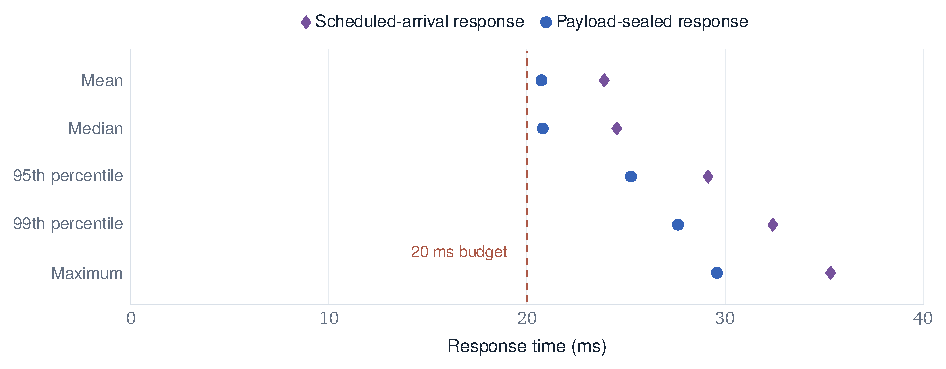
\includegraphics[width=0.98\linewidth]{figures/publication_runtime.pdf}
\caption{\textbf{Historical persistent PHASE reference.} The original 250-update replay has scheduled-arrival p95 29.14\,ms; 201 responses reach or exceed 20\,ms. This figure is not a new Garl comparison. \evidence{L40}}
\end{figure}

All deployment measurements here exclude disk I/O and cover one supplied object region. The initial comparison uses five-second replays; the expanded campaign uses distinct continuous intervals of 3.1--9.3\,s. Neither establishes physical-camera operation, upstream object detection, sixty-second sustained service, multi-object capacity, or calibrated safety decisions. Earlier query-oriented adapter experiments remain in the evidence archive, but their timings are excluded from this article's deployment-latency comparison.
\FloatBarrier

\section{Discussion and limitations}
\subsection{System performance and component attribution}
The private benchmark supports PHASE-TTC as a complete causal TTC system: its archived score improves all four TTC bands relative to the displayed Garl-TTC reference, the only other documented method among the three leaderboard entries. The two systems differ in temporal support, 650\,ms against two observations 0.1\,s apart. An internal control on training folds attributes about three of 85 Overall MiD points to history beyond two slots (Appendix~\ref{sec:post-audit-history}); it does not retrain the reference with longer support, so the difference is bounded within PHASE-TTC and not separated from the architecture. On the same folds, causal box-expansion inputs from the supplied regions halve the head's error (Appendix~\ref{sec:post-audit-geometry}), which indicates that supplied-region history, more than fusion, is where accuracy is available on these folds; whether that transfers to the test set is untested. Our matched transfer tests narrow the explanation. Learned residual readouts outperform equal mixtures and the source-calibrated scalar mixture, yet the 95\% confidence interval for the paired MAE difference between real-event and zero-event heads includes zero, and phase and inverse-TTC corrections give nearly identical mean errors. The refitted heads are also indistinguishable from the RGB branch alone, and the margin over the calibrated mixture depends on one recording. We therefore treat named phase fields as an implementable design choice whose advantage has not been established, and we do not attribute the benchmark gain to event--RGB fusion. Two properties of the evaluated system limit what the null result means: most timing and support fields of the fusion descriptor are constant, and the event branch is evaluated with a history cadence and support count that never occur in its training data (Appendix~\ref{sec:field-ranges}), although matching that cadence at inference does not recover an event benefit (Appendix~\ref{sec:post-audit-event-history}).

The interface still offers a concrete engineering property: each coordinate has a defined meaning across separately fitted producers and out-of-fold rotations. This permits grouped fitting without requiring hidden coordinates to align. Testing whether that property improves accuracy over a matched feature-level fusion model requires an additional comparison. The current benchmark difference also includes changes in upstream estimators, supervision, and temporal history.

\subsection{Adaptation depends on the error regime}
The geometry experiment separates two effects. Adding apparent expansion allows a fixed mixture to recover much of the pooled gain. Learned routing further improves the road subset, where geometric outliers make an unconditional geometric estimate unreliable, but that gain rests on three of eight recordings and on a comparator with fewer experts. Neither aggregate should stand in for the other. The supplied boxes and simplified intersensor projection remain part of this evaluation contract; detector jitter, occlusion, and calibration errors may change the result on new acquisitions.

\subsection{Generalization, reproducibility, and execution}
The private benchmark supplies the only result on targets that development never inspected. The author made one submission to the test server, so no test score informed the recipe; the archive cannot confirm that count independently (Section~\ref{sec:official}). The secondary experiments reuse development-inspected recordings, including the new matched controls. Their three head seeds share the source features and upstream weights. We have no confirmed unused synchronized event--RGB recordings with compatible object-level TTC labels for a new independent test. Additional fits or resampling cannot replace those acquisitions.

For the new 460-query comparison, replaying the released head on recovered features agrees with its saved predictions within $2.87\times10^{-6}$\,s. This local check has a narrower scope than historical full-system reproduction: 504 of 5,805 native-replay queries exceed the original tolerance, with a maximum difference of 0.4968\,s. The original submission and its score remain separately archived, and the drift bounds the benchmark-coordinate change at about 0.01 MiD on average (Section~\ref{sec:official}). The replay discrepancy still requires investigation of the original execution environment and per-query intermediate states; repeatability on the current platform alone cannot resolve it.

The original five-second replay delivers all 250 predictions, but 201 responses meet or exceed 20\,ms and p95 is 29.14\,ms. In the expanded 72-pass study the two-packet policy completes one of 24 PHASE replays and delivers 9.6\% of offered outputs, and the 64-packet queue delivers every output at per-scene p95 responses of 104--227\,ms. The study also exposes scene-dependent queueing, history-gap refusals and numerical disagreements in intermediate PHASE outputs. Increasing the queue preserves more complete deliveries, while native-parity admission and response deadlines remain separate requirements. The historical 26--29\,ms measurements therefore do not establish a universal latency bound. Sustained physical-camera operation, multiple objects, upstream detection, and calibrated warning probabilities remain outside the demonstrated result.

Earlier predictive-learning studies are informative negative experiments, rather than a mechanism explaining the benchmark gain. The recovered scratch, random-frozen, JEPA, and shuffled-future controls appear together in Appendix~\ref{sec:early}. They support the reported failure to demonstrate a JEPA benefit in those settings; they do not identify background appearance as its cause on real data. In the one completed attribution study the frozen JEPA encoder was worse than a frozen random encoder at every label fraction and far behind training from scratch, and the deployed system contains no JEPA-pretrained component.

\section{Conclusion}
PHASE-TTC combines modality-specific motion estimates and temporal context in a compact RGB-anchored readout. Its complete submitted system improves the archived GarlTTC ranking metric by \OfficialOverallRelativeGain{} relative to the Garl-TTC reference, on a three-entry leaderboard and with longer temporal support than that reference. Matched final-head experiments show that a learned correction helps relative to equal mixtures, while event access, phase parameterization, and the correction itself offer no resolved advantage over their matched controls, including the RGB branch alone, on the inspected transfer cohort. Box geometry supplies most of the adaptation gain; learned routing improves road performance beyond a fixed mixture on a few recordings, while the fixed mixture has the lower pooled error. Measured response times exceed the 20\,ms deadline in every configuration tested. These results define an evaluated system and identify the measurements needed to establish broader fusion and deployment claims.
\FloatBarrier

\clearpage
\begingroup\small
\setlength{\bibsep}{3pt}
\bibliographystyle{plainnat}
\bibliography{references}
\endgroup
\appendixdivider
\appendix
\publicationmodefalse
\begingroup\small
\tableofcontents
\endgroup
\clearpage
\section{Implementation and source correspondence}
\label{app:implementation}
The main text uses descriptive component names. The source archive uses A5 for the transport-trained producer, C2F for the coarse-to-fine producer, PAIR for the pairwise temporal readout, and TRAIN40 for the final forty-sequence fit. F0 identifies the frozen base fusion model; F1 identifies a separately fine-tuned fusion head. PHASE17 denotes the context input, whereas PHASE20 denotes the twenty-coordinate fusion interface. These identifiers name different interfaces and are not interchangeable.

\subsection{Final training population and optimization}
Final fitting uses 88,744 TRAIN40 queries from forty sequences. The former P, H, and V groups all contribute to this refit, so their earlier scores characterize development rather than independent validation of the deployed chain. Each producer receives 49,932 updates, equivalent to eighteen epochs at effective batch size 32. The event producers carry forward the earlier TRAIN40 weights; RGB training resumes to the same endpoint. \evidence{L43}

Training comprised 690,934 auxiliary endpoint updates and 58,660 final-head updates across forty-five fits. Final PAIR endpoints used 11,264 updates; each context model and the final head used 12,044. Schedulers and warmup scaled with the fitting population. Update counts describe optimization exposure rather than wall-clock GPU effort.

\subsection{Exact fusion layout and emission policy}

Each context refiner is represented for final fusion by a constructed 170-coordinate block. Coordinates 0--159 are its learned hidden state. Coordinates 160--169 are an explicit interface containing, in order, one raw location, one emitted phase, three expert phases, four current timing values, and one valid-history count divided by eight. Concatenating the RGB block followed by the event block gives the 340-coordinate container
\begin{equation}
  \mathbf{s}=\left[\mathbf{s}_{R}^{170};\mathbf{s}_{E}^{170}\right]\in\mathbb{R}^{340}.
\end{equation}
Fusion reads \(\mathbf{s}_{160:170}\) and \(\mathbf{s}_{330:340}\), yielding twenty named phase, timing, and support inputs while the 160-dimensional hidden states remain within their modality branches. Within each ten-coordinate block, the first five phase coordinates are divided by \(0.03\); timing and support keep their native scaling. The shared interface aligns quantities with consistent meanings across the separately fitted refiners. \evidence{M22}

The selected vector passes through
\begin{equation}
  20\rightarrow 32\;[\mathrm{LayerNorm},\mathrm{SiLU}]
  \rightarrow 32\;[\mathrm{LayerNorm},\mathrm{SiLU}]
  \rightarrow 3.
\end{equation}
Zero initialization of the last affine layer makes the initial fusion output equal to the RGB anchor. If \(c_0,c_1,c_2\) are the three head outputs, \(\ell_R\) is the RGB raw-location anchor, and \(\mathbf{w}_R\) is the separately supplied pair of RGB width logits, the deployed computation is
\begin{align}
  \ell_F &= \ell_R + 0.03c_0, \\
  \boldsymbol{\sigma}_F &= 0.03\,\operatorname{softplus}\!\left(\mathbf{w}_R+[c_1,c_2]\right), \\
  \widehat{\mathrm{TTC}} &= \operatorname{phase\_to\_ttc}(\ell_F), \\
  q_{10}^{\phi} &= \operatorname{clip}(\ell_F-\sigma_{F,0},\,\phi_{\min},\phi_{\max}), \\
  q_{90}^{\phi} &= \operatorname{clip}(\ell_F+\sigma_{F,1},\,\phi_{\min},\phi_{\max}).
\end{align}
The native bounds are \(\phi_{\min}=-\log 2+10^{-6}\) and \(\phi_{\max}=8\). For the point prediction, the inverse map clamps \(\ell_F\) to these bounds, computes \(q=-\operatorname{expm1}(-\phi)/0.1\), and emits \(\operatorname{sgn}_{+}(q)/\max(|q|,1/60)\) seconds, where \(\operatorname{sgn}_{+}(0)=1\). Thus the emitted magnitude is at most 60\,s and zero phase maps to \(+60\)\,s. The reported point phase is recomputed from this finite TTC; the learned-width phase-interval endpoints are clamped separately. The rate floor keeps inversion finite near zero expansion, imposing a nominal signed horizon of 60\,s. \evidence{M22,R02}

The compact fusion head contains 1,955 trainable parameters: \(672+64+1{,}056+64+99\) across three affine layers and two LayerNorms. Figure~\ref{fig:fusion-layout} summarizes the named-field and anchor paths. \evidence{M22}

\begin{figure}[H]
  \centering
  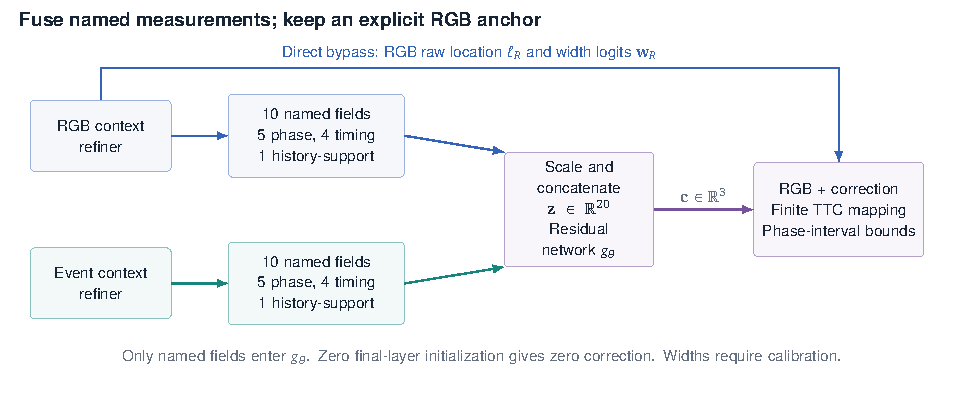
\includegraphics[width=\linewidth]{figures/publication_fusion.pdf}
  \caption{\textbf{Named-feature fusion interface.} The twenty selected coordinates enter the correction network. RGB location and width logits bypass that network and combine with its three outputs. \evidence{M22}}
  \label{fig:fusion-layout}
\end{figure}


\subsection{Transfer target association and eligibility}\label{app:target-association}
The historical transfer registered sixteen uniformly spaced queries in each of thirty-two EvTTC sequences, together with forty-six earlier queries. Four duplicate identities were removed, leaving 554 saved candidates: 46 Historical46 and 508 Extended-new. The associated object is the primary annotated object matched to the scenario's scalar TTC series; the public projection does not establish arbitrary per-object TTC correspondence.

The original assignment interchanged the low-100 and medium-100 TTC sources for the two CCRs-1 recordings. The later public-source audit fixes their identities by download mapping and SHA-256. An independent RGB-identity record links the competition extracts to the same native recordings, matching all 50 low and 43 medium frames with constant competition-to-native offsets. Transfer queries already use native microseconds, so no additional offset is fitted or applied. \evidence{GT01}

All 508 Extended-new candidates are reassociated, including the forty previously excluded queries. The matching rule remains nearest public TTC within 50\,ms, with the earlier timestamp breaking ties. The low and medium groups each contributed fifteen previously scored queries; they now contribute ten and twelve. Historical46 does not contain these groups and retains its 46 eligible queries.

Table~\ref{tab:audit-transfer-eligibility} lists the candidate and eligibility counts for every sequence group.

The revised Extended-new denominator is therefore \AuditTransferCount{}, with 48 exclusions across the original 508 candidates. All retained targets are positive. Every query anchor and every model prediction remains unchanged. The historical 468-query ledger is preserved in \path{data/transfer_queries.csv}; current results use \path{audit_20261104/corrected_transfer_candidates.csv}. The associated receipt records the original and corrected source hashes and the neighboring label timestamps for each reassociation. \evidence{GT01}


\section{Competition inputs: historical coverage and disagreement}
\label{sec:evttc-competition}
\cohortline{28 OCTOBER INFERENCE SNAPSHOT / 434 query identities / 10 sequences / coverage and prediction disagreement}
We applied three released Garl-TTC variants to the same ten-sequence EvTTC inputs as the frozen PHASE-TTC reference. The 434 queries span eight road and two Slider sequences, with sequence, row, frame index, and timestamp matched across models. The comparison contains 1,302 Garl outputs and 434 PHASE-TTC outputs. \evidence{T01}

At the time of this frozen inference comparison, no verified numeric TTC targets mapped to the 434 query identities. The analysis therefore measured coverage and paired prediction disagreement:
\begin{equation}
d_i^{(m)}=\widehat T_{i,m}^{\rm Garl}-\widehat T_i^{\rm PHASE},\qquad a_i^{(m)}=|d_i^{(m)}|.
\label{eq:evttc-disagreement}
\end{equation}
The differences in Equation~\ref{eq:evttc-disagreement} compare model outputs rather than prediction error. This population differs from both the labeled transfer in Section~\ref{sec:late-transfer} and Garl's published three-sequence RTE evaluation. Appendix~\ref{app:competition-details} gives the adapter, timing measurements, and ten sequence traces.

The corrected target audit reported on 1 November supersedes the earlier absence of local labels: it recovers all 434 targets after resolving the public source assignment for two road sequences. Section~\ref{sec:quality-adaptation} uses those targets to compare original and adapted PHASE-TTC under one documented local evaluator. The results below preserve the original Garl-versus-PHASE outputs and their coverage rather than retroactively presenting them as a reproduced error ranking. The published three-sequence result remains a separate protocol, and the Slider-750 discrepancy prevents claiming official equivalence for the new local scores. \evidence{T01,T02,N01}

\subsection{Frozen checkpoints and native input support}
The released full, event-only, and visual-only state dictionaries load strictly and run in float32 with frozen weights. RGB-dependent routes use two real causal frames, while event-only uses two observed causal intervals. Startup queries without the required observations remain unavailable. PHASE-TTC uses up to 650\,ms of context, so the models share query identities under different temporal support. \evidence{T01}

Supplied boxes and calibration condition each route. Rotation-only projection omits translation because object depth is unavailable. For Slider, the adapter derives rotation from the supplied camera poses because the data provide no named event-to-RGB extrinsic. We treat the resulting runs as frozen-checkpoint adaptations.

\subsection{Coverage, sign, and disagreement tails}
\begin{table}[tbp]
\centering\small
\caption{Predictions on 434 EvTTC competition queries. The table reports finite-output coverage, signed TTC range, and negative counts. Median and P95 summarize absolute differences from PHASE-TTC where both models produce finite outputs. \evidence{T01}}
\label{tab:evttc-model-summary}
\begin{tabular}{@{}lrrrrr@{}}
\toprule
\textbf{Model} & \textbf{Finite} & \textbf{Range (s)} & \textbf{$<0$} & \textbf{Median (s)} & \textbf{P95 (s)} \\
\midrule
PHASE-TTC & 434/434 & [-42.225, 51.869] & 2 & -- & -- \\
Garl full & 424/434 & [0.907, 52.705] & 0 & 0.261 & 1.098 \\
Garl event-only & 434/434 & [-42.211, 406.095] & 10 & 0.681 & 5.623 \\
Garl visual-only & 426/434 & [-23.832, 38.767] & 5 & 0.236 & 1.524 \\
\bottomrule
\end{tabular}
\end{table}

PHASE-TTC and event-only Garl each emit 434 finite values; full Garl emits 424 and visual-only 426. The first query in each road sequence lacks two causal RGB frames, creating eight gaps in both RGB-dependent variants. Full Garl has two further Slider-750 gaps because the earlier event endpoint precedes recorded coverage. All invoked models return finite values; nulls correspond to unavailable inputs.

\begin{figure}[htbp]
\centering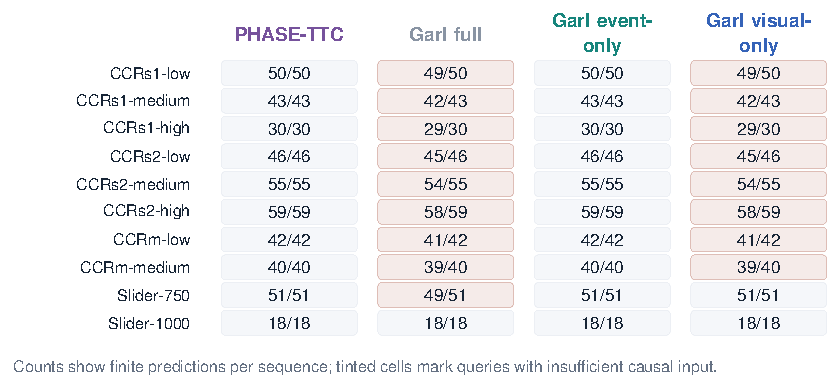
\includegraphics[width=\linewidth]{figures/rev_coverage.pdf}
\caption{\textbf{Finite prediction coverage by model and sequence.} Tinted cells mark the eight missing road RGB pairs and two additional early Slider-750 event gaps in full Garl. \evidence{T01}}
\label{fig:evttc-coverage}
\end{figure}

On shared finite rows, median absolute disagreement from PHASE-TTC is 0.26\,s for full Garl, 0.68\,s for event-only, and 0.24\,s for visual-only. Their p95 disagreements are 1.10, 5.62, and 1.52\,s. Full Garl emits no negative TTC, compared with two negative PHASE-TTC outputs, ten event-only outputs, and five visual-only outputs. \evidence{T01}

Slider-750 contains the largest excursions: event-only reaches 406.10\,s, with p95 absolute disagreement of 241.68\,s. The native height-ratio conversion becomes ill-conditioned as the two predicted endpoint heights approach equality. Figures~\ref{fig:evttc-predictions-symlog} and~\ref{fig:evttc-predictions-linear} preserve the sign and magnitude of these outputs across all ten sequences. \evidence{T01}

Timing remains descriptive because the variants ran once in fixed order with shared cache and warm-state effects, and PHASE-TTC used a different adapter and longer history. \evidence{T01}
\FloatBarrier

\section{Adaptation lineage and calibration controls}
\label{app:adaptation-lineage}
\subsection{Adaptation lineage and rejected candidates}
The name ``adapted PHASE'' refers to several checkpoints with different fitting populations. F0 denotes the original nine-component TRAIN40 graph. The first F1 adaptation updates its original 1,955-parameter fusion head while freezing the eight preceding components and their normalizers. Its all-32-recording refit uses 88,744 TRAIN40 OOF states and 3,571 admitted EvTTC states, for 92,315 training rows; 257 native queries lack compatible targets. Each of seeds 7, 13, and 21 completes two epochs and 1,444 updates, with seed 7 designated for delivery before scoring. These are training-fit results. \evidence{A01}

The preserved all-32 F1 cache confirms that its supervision consumed the old CCRs1-low/medium source assignment. Its preparation script reads each query's \texttt{ttc\_csv\_path}, hashes the file, and joins its TTC curve before writing supervised shards. The preserved \texttt{data\_v3/TARGET\_LEDGER.json} records the old low-file hash beginning \texttt{780ee30f} and medium-file hash beginning \texttt{1c5adba8}; under the corrected identity map those files belong to medium and low, respectively. It admits 98 low and 141 medium queries, with two and eight additional unsupported targets. Its completion receipt binds both that ledger and the merged training array, and the three seeds' start receipts and delivered seed-7 bundle bind the same completion receipt. Thus 239 admitted supervised rows used the old map, and the ten exclusions also require a new eligibility check. Rescoring retained outputs cannot repair those F1 weights: a corrected all-32 F1 requires rebuilding the supervised cache and refitting seeds 7/13/21. No corrected all-32 F1 training is reported here. The grouped F1 campaign below excludes the eight overlapping competition recordings, including these two recordings, and restarts from F0 in each fold. This particular source swap does not invalidate that grouped comparison or establish a dependency in the final 688-parameter router, whose optimizer population excludes those recordings. \evidence{A01,A02}

That grouped campaign comprises 21 head fits: seven scenario families times three seeds, with 2,531 queries from twenty-four road recordings. It retains TRAIN40 during each fit. F1 reduces recording-macro RAE from F0's 30.600\% to 25.468/26.188/25.938\%, but increases query MAE from 0.8494\,s to 0.8585/0.8925/0.8653\,s for seeds 7/13/21. All three family-bootstrap intervals for the RAE difference include zero. For targets above 4\,s, seed 7 increases MAE from 1.2542 to 1.5496\,s. On Slider-500, outside this optimizer fit but historically exposed, F1 increases RAE from 83.887\% to 87.578/91.022/87.330\%; each variant returns 76 of 77 outputs. Lower road relative error therefore did not establish uniform improvement. \evidence{A02}

The next quality-fusion campaign freezes all nine F0 components and fits three 401-parameter gates. Its named \texttt{evaluated} checkpoint has separate fitting, calibration, and confirmation roles; \texttt{all\_data\_refit} instead consumes all 2,677 eligible queries from twenty-four road and three Slider recordings. The latter's reported errors are resubstitution. On 1,747 road OOF queries, the quality gate gives RAE 12.834\% and MAE 0.4224\,s, versus 22.081\% and 0.7544\,s for an equal-parameter control without quality descriptors. Both receive geometry. This supports quality information for that gate and population. \evidence{A03}

The preserved bundles close the upstream-weight distinction: the 401-parameter gate, startup router, and submitted router all bind the original F0 head. Hash checks of their thirteen upstream components, including normalizers and seal/recipe records, agree with their manifests. None substitutes the affected all-32 F1 heads; complete checkpoint identities and cache bindings are retained in the additional source index. The gate preparation explicitly selects F0, RGB context, and event context as native experts; startup reuses those experts, and submission refits the router while copying the verified original upstream bundle. This establishes a separate weight lineage, while retaining the historical data exposure of all three gate campaigns. \evidence{A01,A03,A04,A07}

The startup campaign then executes 117 fits, including Q/QA/NAcap controls, seconds- and inverse-coordinate trials, and all-data refits. It retains the 688-parameter inverse-coordinate router as a candidate after rejecting the seconds-coordinate trial. Road OOF MAE changes from the previous gate's 0.4224 to 0.4049\,s, while CCRm confirmation MAE worsens from 1.020 to 1.036\,s. Its descriptive road RAE-difference interval, resampling five families, is $[-1.5176,0.8001]$ percentage points. Development now includes Slider-750/1000, so this comparison changes both architecture and exposure. The final submitted recipe below returns to a 2,608-query optimizer population; earlier use of those Slider recordings still counts as design exposure. \evidence{A04}

A further 312 completed small-head fits test sign/log/geometry variants (96), supervised cost (48), correlated expert perturbations (24), native-context resets (48), support versus capacity (48), and support with resets (48). Eight family-held-out folds, seeds 7/13/21, and 300 updates per fit use the 2,608-query population. Promotion requires full coverage and no worsening of both recording-macro RAE and MAE in either road or Slider relative to IQ. None passes all four error criteria. The six preserved fits from an earlier failed launch do not enter the 312 total. The 447 context resets cover 149 prepared queries; they do not represent 447 cold sensor starts. These fits are separate from the 21 F1 fits, the 117 startup fits, and the later 48 canonical-router fits. \evidence{A05}

\subsection{Measured interval coverage by variant}
The grouped F1 experiment also measures substantial undercoverage. Its nominal 80\% intervals cover 67.88/65.78/67.72\% for seeds 7/13/21. Rescaling with each fold's training residuals raises coverage only to 70.17/68.63/70.01\%; that procedure is not split conformal and was not bundled. The earlier 401-parameter \texttt{evaluated} gate uses separate CPNAO calibration records and attains 79.83\% CCRm coverage. The startup \texttt{evaluated} candidate reports 83.10\% CCRm coverage after separate CPNAO calibration. These are descriptive results on historically exposed groups. Their all-data refits consume those calibration labels and carry no validated equivalent interval; neither does the final 2,608-query submitted router. Finite-output coverage and probabilistic interval coverage describe different properties. \evidence{A02,A03,A04,A07}


\subsection{Geometry controls and support differences}
\label{app:geometry-attribution}
F0 versus the final router changes both the available experts and the learned combination. The older 401-parameter capacity control establishes a benefit of quality descriptors only within its own experiment. Its Slider-750 geometry observer has MAE 0.1976\,s on 49/51 outputs, versus 3.3157\,s for that gate on 51/51; Slider-1000 gives 0.0374\,s on 16/18 versus 0.2757\,s on 18/18. Different masks prevent a direct attribution from these aggregates. The new common-support comparison in Section~\ref{sec:quality-adaptation} now evaluates geometry, fallback, fixed mixture, and the final router on these saved inputs. It supplies the matched attribution that the earlier aggregate records lacked. \evidence{A03,N01}

\section{Canonical cadence as a controlled intervention}
\label{sec:canonical-cadence}
\cohortline{FROZEN-GRAPH INTERVENTION / 149-query screen and 2,608-query development population / candidate not promoted}

The metric phase uses a fixed interval, whereas the sensor supplies observations at measured intervals. These two time quantities must remain separate. The canonical-PAIR experiment asks whether normalizing the learned readout to a reference interval improves its consistency, then tests whether any local improvement survives the downstream contexts and fusion. The intervention introduces no optimizer updates into the original chain. \evidence{N02}

\subsection{Recomputing the readout before rescaling}
The intervention first rebuilds the 133-coordinate PAIR input with its three time-derived fields recomputed for $d_0=0.1$\,s: duration, log-duration, and inverse duration. The frozen PAIR network processes this input and emits raw phase $\phi_c$. Given the actual interval $\Delta$, the adapter then computes
\begin{align}
 q_c&=-\operatorname{expm1}(-\phi_c)/d_0,\\
 q_\Delta&=q_c d_0/\Delta,\\
 \phi_\Delta&=-\log(1-d_0q_\Delta).
 \label{eq:canonical-pair-intervention}
\end{align}
Only after this transformation does it apply the original emission policy. The implementation checks finiteness and $1-d_0q_\Delta>0$; unsupported transformations remain explicit failures. When $\Delta$ equals the FP32 representation of 0.1\,s, a direct identity path preserves the original bytes. This is not a division of an already emitted TTC, nor a rescaling of the original phase with its time-conditioned features unchanged. \evidence{N02}

Weights, normalizers, observation cutoffs, and producer batches remain fixed. The run reconstructs the complete PHASE17 feature vector from corrected PAIR features, including disagreements, and reruns temporal contexts and the final fusion head. Predictions and missing-output status are sealed before a separate process joins targets. Each new query first reproduces a paired original execution on the same platform; an old cache is not substituted as the control.

A small time-warp diagnostic motivated this population test. It altered prepared observations and their clocks, rather than reselecting fixed-duration windows from a time-scaled raw stream. Under speed factor $a$, the ideal comparison is $aT_{\mathrm{warped}}/T_{\mathrm{original}}=1$. Canonicalization improved all four tested F0 contrasts, yet the road event-context ratio at $a=0.5$ moved from 0.6738 to 1.891. The downstream regression prevents an interpretation in which every intermediate correction must benefit the complete estimator. \evidence{N02}

\subsection{Fixed screen and modality localization}
The initial screen contains 72 road queries and 77 Slider-500 queries. A later four-arm localization control holds this population fixed and corrects events only, RGB only, both, or neither. In that paired CPU control, road macro MAE is 0.7489\,s for the original and event-only arms, and 0.7487\,s for RGB-only and both. The observed road change therefore comes from the RGB intervention in this control. On the 76 available Slider outputs, the corresponding values are 1.178, 1.163, 1.142, and 1.121\,s. Both modalities contribute there. This localization experiment diagnoses a fixed candidate; it does not select a new recipe after inspecting the four results. \evidence{N02,N05}

\subsection{Complete development population}
\EvidenceCanonicalTable
The full experiment reuses the sealed screen and adds 2,459 road queries, yielding 2,531 road queries across twenty-four recordings and 77 Slider-500 queries. The original F0 and its canonical counterpart both return all road predictions and 76 Slider predictions. The previous Slider absence remains absent. Neither route introduces a new missing prediction or a sign change. \evidence{N02}

Road recording-macro MAE changes from 0.8106 to 0.8105\,s, a reduction of 0.13\,ms. A paired bootstrap over complete road recordings, using 10,000 resamples and seed 7, gives a descriptive 95\% difference interval of $[-0.50,0.09]$\,ms. The interval includes zero. Slider-500 improves from 1.1782 to 1.1208\,s, a 4.87\% relative reduction on one acquisition already inspected in the screen. Table values retain the original precision.

The original fused estimator, denoted F0, satisfies the fixed numerical development criteria: preserve coverage, avoid worsening either error metric in either domain, and improve at least one metric. The small road effect and reuse of development recordings motivate the downstream router and refitting comparisons below.

\subsection{Propagation through the quality router}
The frozen adapted router improves aggregates on the complete population but fails the earlier road screen. That failed criterion remains binding. A subsequent paired refit evaluates eight folds, three seeds, and original/canonical feature arms, totaling 48 fits. The canonical ensemble improves full-population road MAE from 0.5396 to 0.5378\,s and Slider MAE from 0.3650 to 0.3565\,s. On the fixed screen, however, road MAE worsens from 0.4848 to 0.5118\,s and relative error from 16.72\% to 17.43\%. No seed passes both evaluation views. The fixed-screen degradation excludes this refit under the combined selection criteria, so the delivered PHASE-TTC-Adapt recipe is retained. The comparison concerns out-of-fold ensembles; the delivered router is fitted on the complete adaptation population. \evidence{N03}

\subsection{Native replay: output sensitivity versus accuracy}
The same-platform eAP comparison covers 5,805 physical queries and their 6,762 submission-template tokens, including aliases. Both arms preserve availability and sign, and the event context remains identical. For F0, median absolute output change is $1.4305\times10^{-5}$\,s, p95 is $7.6771\times10^{-5}$\,s, and the maximum is 0.006496\,s. These are differences between model predictions, not errors relative to targets. The private Test12 labels were not used, so the experiment establishes no accuracy or ranking conservation. \evidence{N03}

Historical parity is a separate issue. The recaptured original is exactly repeatable locally, but every one of the 5,805 queries fails some comparison with historical intermediate states, and 504 fail the historical TTC tolerance. Local repeatability cannot remove those failures or assign their cause. The paired original/canonical design isolates the new intervention within the present platform while retaining the older reproducibility discrepancy.

Across those 5,805 original-output comparisons, the absolute historical-to-local TTC difference has median 0.0001855\,s, p95 0.001094\,s, p99 0.002797\,s, and maximum 0.4968\,s. The 504 TTC failures represent 8.68\% of queries. These magnitudes describe reproducibility drift without reading private targets; they are not accuracy errors and do not show that drift caused the local canonical change. The maximum also prevents extrapolating the small same-platform canonical deltas to numerical conservation of the submitted historical run. \evidence{A08}

A separate 120-query warm-weight adapter experiment found an execution-cost regression for the canonical intervention. Its original measurements remain in source N07, but they do not use the persistent service and are excluded from this article's latency comparison. The failed cost criterion and lack of sustained-service evidence remain part of the intervention's historical assessment. Section~\ref{sec:runtime} reports persistent-service response.
\evidence{N07}
\FloatBarrier

\section{Technical foundations and historical method families}
\label{sec:methods}

PHASE-TTC grew through four model families: predictive embedding, geometry-constrained endpoint estimation, phase-domain temporal refinement, and RGB-anchored event fusion. Each family tests a different mechanism with its own objective and inference path. \evidence{M01--M14}

\begin{figure}[H]
\centering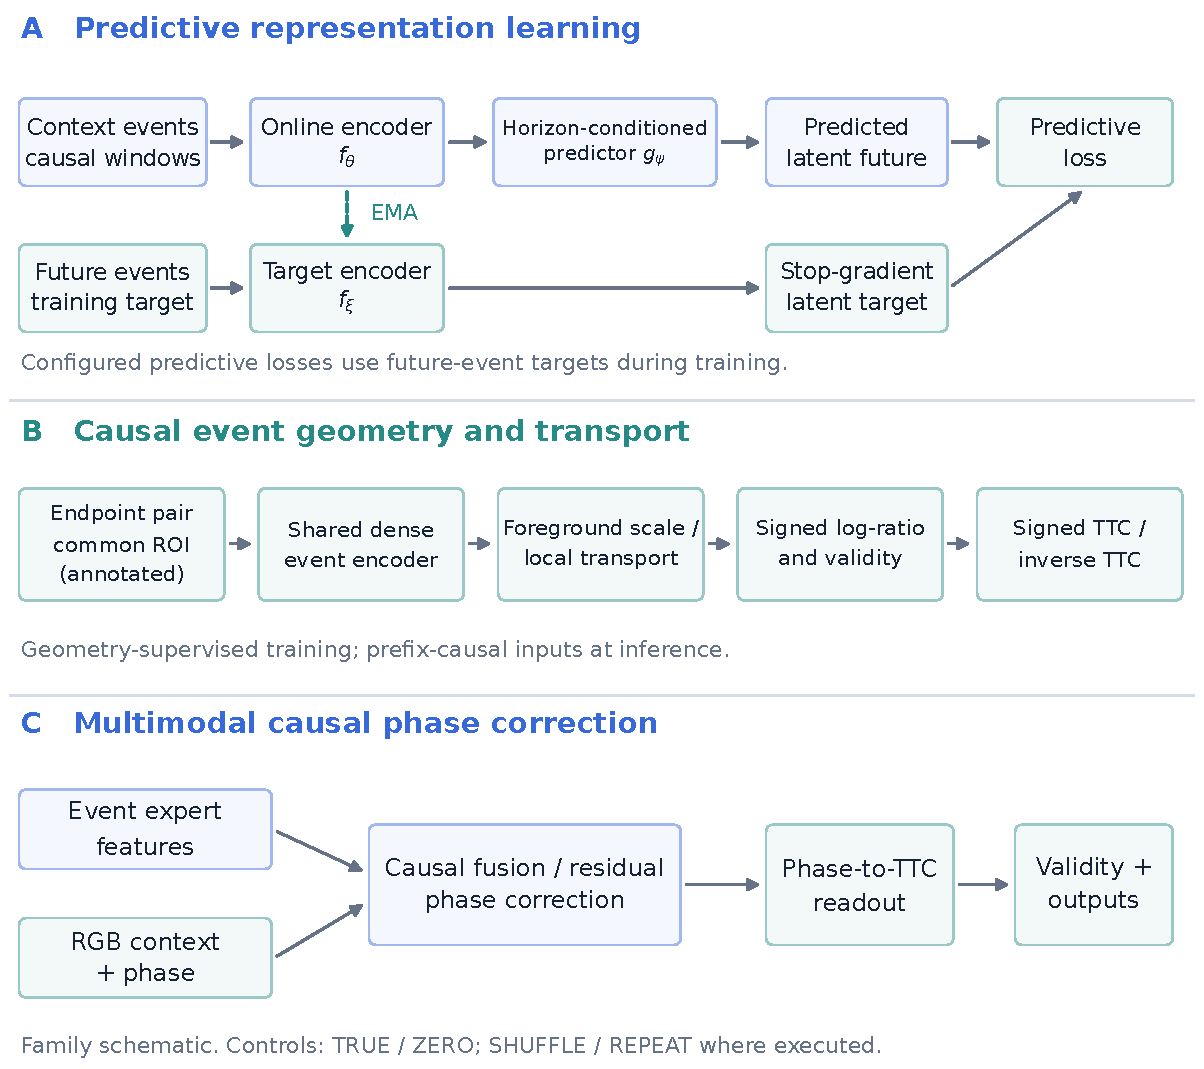
\includegraphics[width=\linewidth,height=.80\textheight,keepaspectratio]{figures/architecture.pdf}
\caption{\textbf{Selected model families.} (A) Predictive latent learning uses a training-only target branch. (B) Causal scale and transport map endpoint geometry to signed motion. (C) Phase-domain fusion combines event and RGB evidence. Panel A contains the JEPA objective; Sections~\ref{sec:phase-refinement} and~\ref{sec:train40} detail the later temporal and fusion paths.}
\label{fig:architecture}
\end{figure}
\FloatBarrier

\subsection{Events, temporal windows, and object coordinates}
An event stream is a sequence $\mathcal E=\{(x_i,y_i,t_i,p_i)\}_{i=1}^N$, with integer microsecond timestamps and normalized polarity $p_i\in\{-1,+1\}$. \texttt{EventBatch} stores aligned NumPy arrays for these fields. Each context window is anchored at its end time. Indexing rejects nonpositive durations, mismatched reference times, and future windows that begin before context ends. Causality tests cover crops, features, checkpoints, and calibration inputs. \evidence{M01}

The dense voxel representation distributes an event between adjacent temporal bins. For $K$ bins, duration $\Delta t$, and normalized time $u_i=(K-1)(t_i-t_0)/\Delta t$, the unnormalized representation is
\begin{equation}
 V_{p,k}(x,y)=\sum_i \mathbf 1[x_i=x,y_i=y,p_i=p]\max(0,1-|u_i-k|).
\end{equation}
Separate polarity yields $2K$ channels. Two flattened weighted histograms accumulate the adjacent-bin contributions without constructing a buffer with twice the event count. Optional robust scaling divides occupied voxels by the 95th percentile of their absolute magnitude; empty voxels remain zero. Median centering is omitted because equal occupied counts would collapse to zero. Event count, time surface, and sparse tokens remain separate representation alternatives. \evidence{M02}

Object-centred experiments use a common square region that covers both endpoint boxes, expands by a fixed margin, and maps both event windows into one raster coordinate system. Tight independent crops can erase apparent scale change. The resulting tensor is \emph{oracle-box-conditioned}: the event backbone assumes external localization even though its forward signature has no box argument. Causal-scale tests confirm that only the designated endpoint boxes affect the crop. \evidence{M03}

\begin{figure}[tbp]
\centering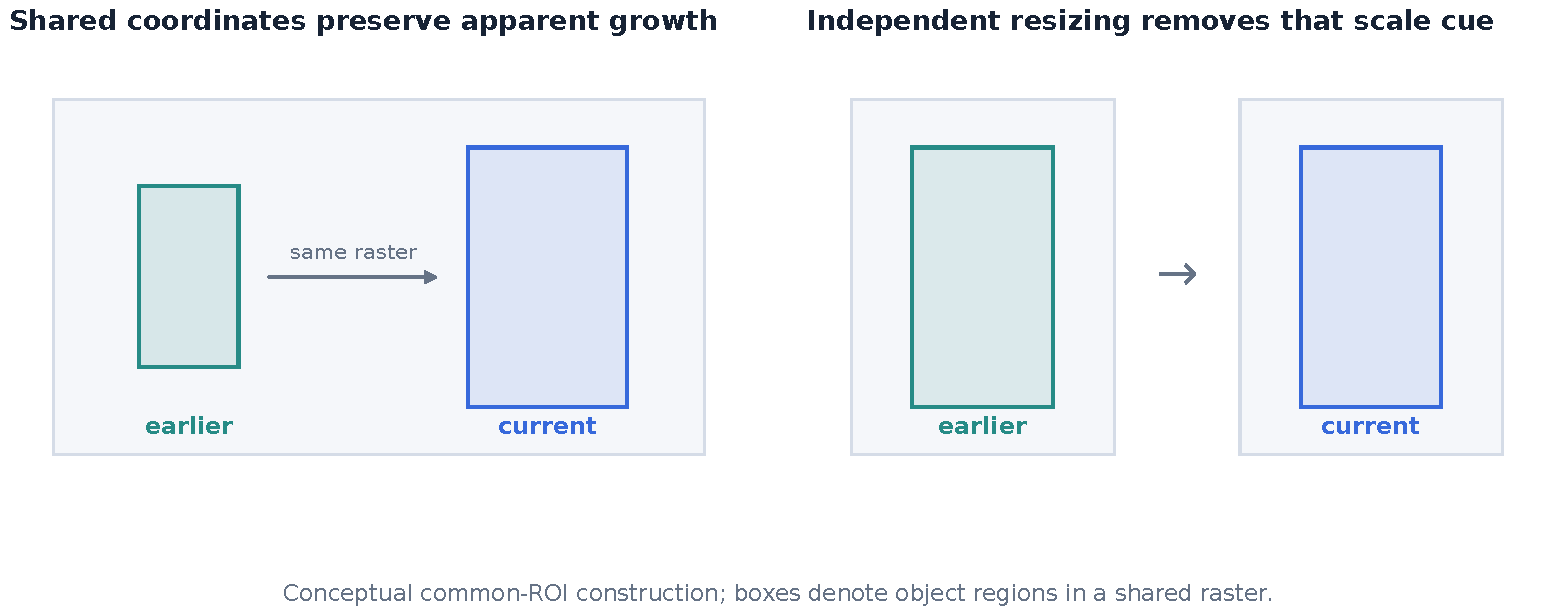
\includegraphics[width=\linewidth]{figures/crop_geometry.pdf}
\caption{\textbf{Shared coordinates preserve apparent expansion.} A common crop maps both endpoints at one spatial scale, whereas independent tight crops normalize away part of the size change. The diagram is schematic.}
\label{fig:crop}
\end{figure}

\begin{figure}[tbp]
\centering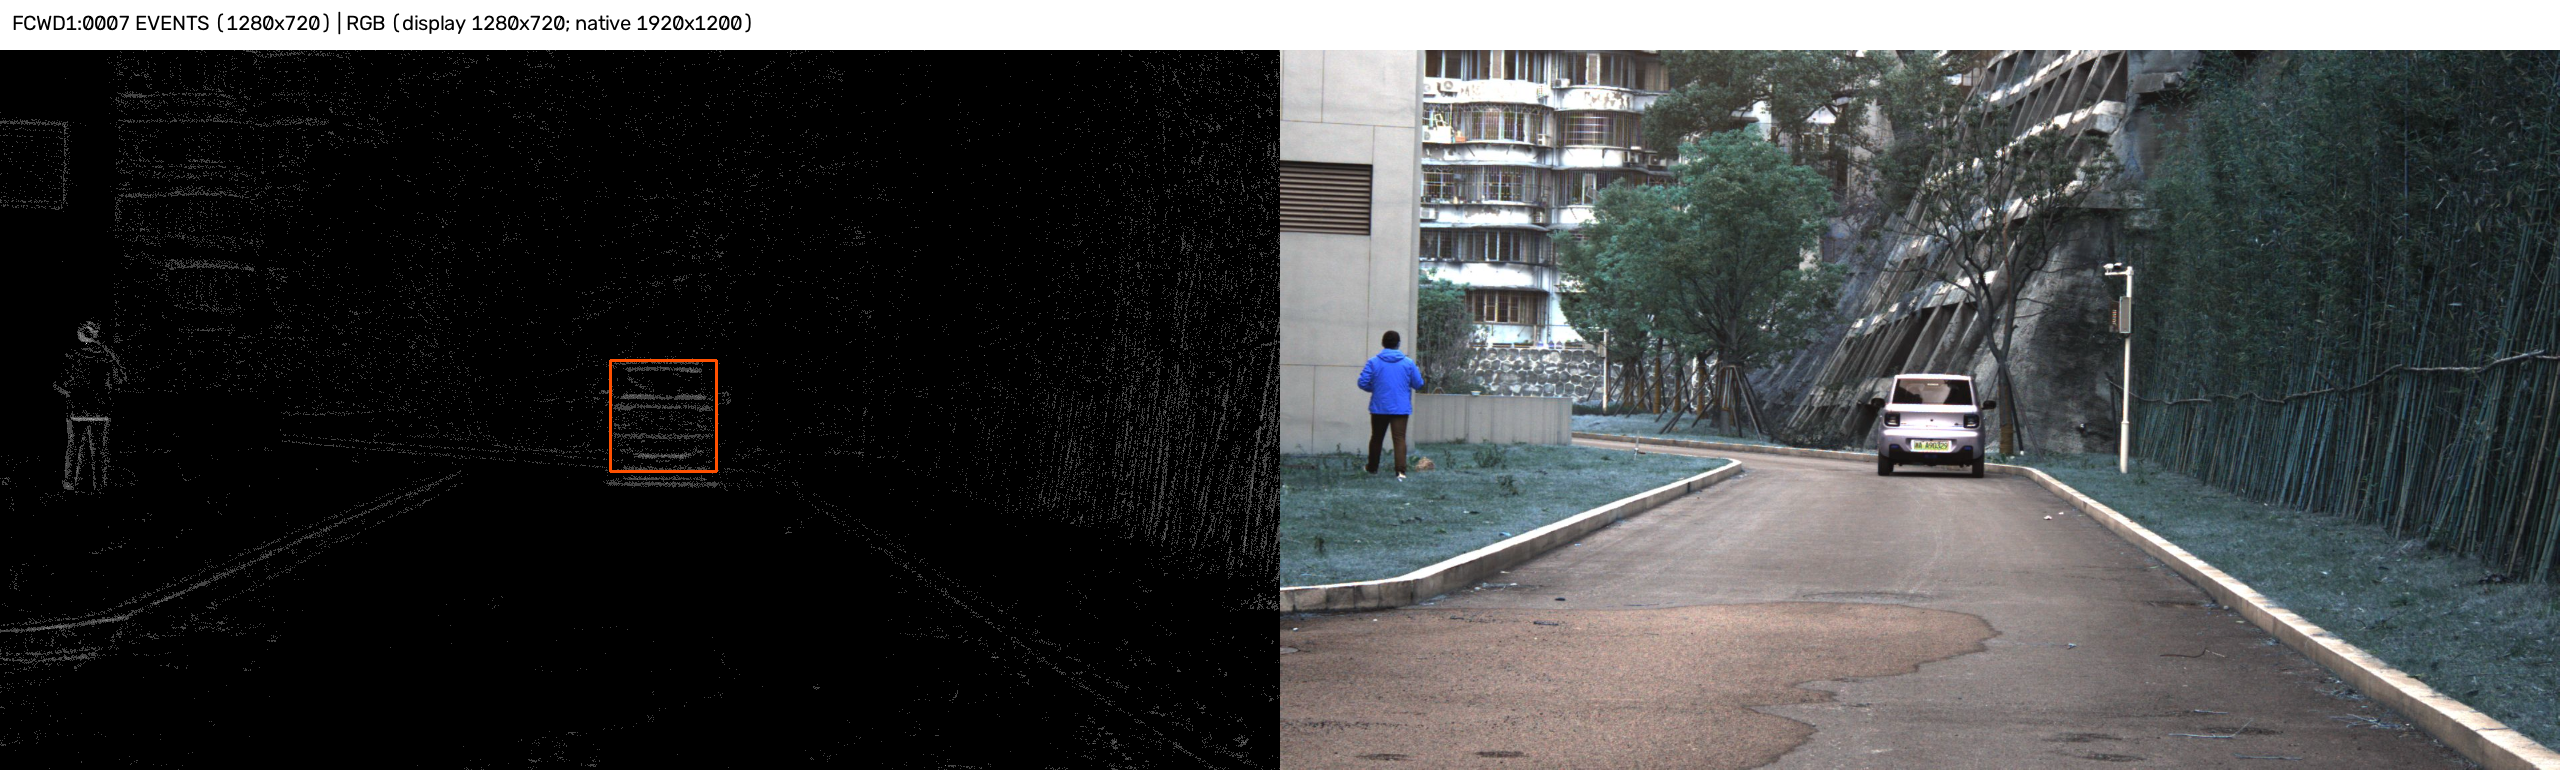
\includegraphics[width=\linewidth]{figures/fcwd_example.png}
\caption{\textbf{Event and RGB appearance for one object region.} FCWD1:0007 illustrates the cross-modal alignment problem. The orange region is the original visualization overlay.}
\label{fig:sensors}
\end{figure}

The eAP adapter reconstructs local targets from public three-dimensional tracks, whereas the benchmark uses private smoothed labels. Results therefore keep reconstructed eAP targets, EvTTC labels, and official GarlTTC labels in separate evaluation populations. \evidence{M01}

\subsection{Real temporal crops and event input planes}
\label{sec:real-inputs}

Figure~\ref{fig:real-evttc-triplets} follows the same EvTTC vehicle at three recorded queries. Each row shows three causal endpoints in a shared object-centred coordinate system for its modality. The RGB square covers the last two supplied boxes with a 25\% margin; event crops use the manifest's event-camera square. Coordinates are shared across endpoints within each modality, not across the two physical cameras. The displayed triplets are input excerpts, not the complete 650\,ms context history.

\begin{figure}[H]
  \centering
  \begin{tabular}{@{}p{.485\linewidth}@{\hspace{.03\linewidth}}p{.485\linewidth}@{}}
    \centering\small\textbf{RGB endpoint crops} & \centering\arraybackslash\small\textbf{Event endpoint crops} \\
    \multicolumn{2}{@{}l@{}}{\small Query 00: anchor $t=14.350374$\,s} \\
    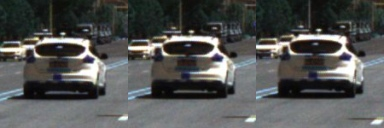
\includegraphics[width=\linewidth]{figures/evttc_query-00-rgb.jpg} &
    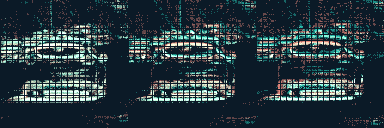
\includegraphics[width=\linewidth]{figures/evttc_query-00-events.png} \\[5pt]
    \multicolumn{2}{@{}l@{}}{\small Query 07: anchor $t=16.800436$\,s} \\
    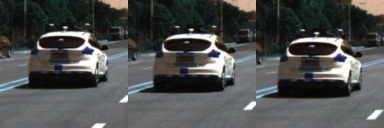
\includegraphics[width=\linewidth]{figures/evttc_query-07-rgb.jpg} &
    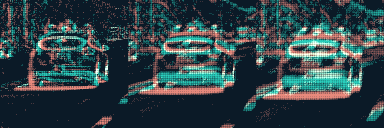
\includegraphics[width=\linewidth]{figures/evttc_query-07-events.png} \\[5pt]
    \multicolumn{2}{@{}l@{}}{\small Query 15: anchor $t=20.450520$\,s} \\
    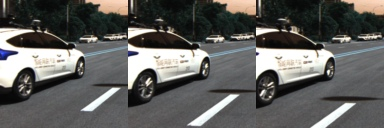
\includegraphics[width=\linewidth]{figures/evttc_query-15-rgb.jpg} &
    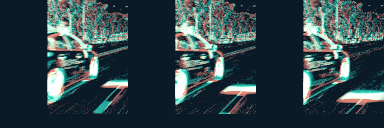
\includegraphics[width=\linewidth]{figures/evttc_query-15-events.png}
  \end{tabular}
  \caption{\textbf{Actual temporal inputs from the EvTTC road excerpt.} Each strip contains three $128\!\times\!128$ crops, ordered from oldest to newest. Event windows end at $t-200\,\mathrm{ms}$, $t-100\,\mathrm{ms}$, and $t$, where $t$ is the stated anchor; each accumulates the preceding 100\,ms. The RGB frame timestamps differ from the corresponding event endpoints by at most 7\,$\mu$s in these examples; exact times are preserved in the source sidecar. Turquoise and coral denote positive and negative event counts with per-crop log display scaling. RGB crops preserve the frozen runtime's stored channel order; JPEG images are visual encodings, not lossless tensors. Source: EvTTC \citep{evttc}, \texttt{CCRm-low-0-overlap-0}; queries are selected illustrations from the previously exposed transfer cohort.}
  \label{fig:real-evttc-triplets}
\end{figure}

Figure~\ref{fig:real-evttc-channels} separates the latest event crop of query 07 into the planes produced by the runtime encoder. This distinguishes the polarity display used above from the actual twelve-channel representation. The voxel planes retain temporal structure within the accumulation window; count and rate planes provide additional support measurements. These are preprocessing outputs, not learned feature maps or neural activations.

\begin{figure}[H]
  \centering
  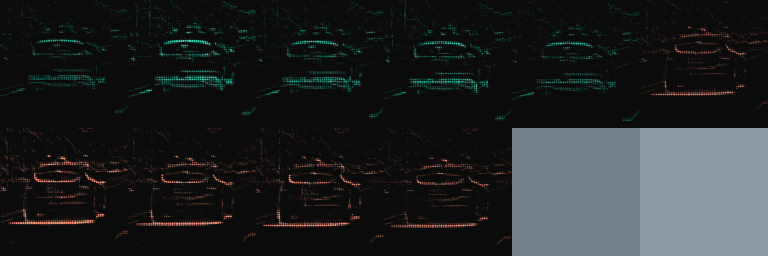
\includegraphics[width=\linewidth]{figures/evttc_query-07-channels.png}
  \caption{\textbf{Twelve event input channels from a real measurement.} Query 07, window $[16.700436,16.800436)$\,s. Reading left to right across the upper row gives positive voxel bins 1--5 and negative bin 1; the lower row gives negative bins 2--5, log event count, and log event rate. Each tile is $128\!\times\!128$ pixels. Display values are clipped to $[0,2]$ for voxel planes and $[0,20]$ for count/rate planes, then colorized; the saved sidecar retains the unclipped per-plane minimum, maximum, and mean. The two support planes appear nearly uniform at this display scale. Source: EvTTC \citep{evttc}; extracted with the frozen runtime's \texttt{map\_roi\_lut} and \texttt{encode\_mapped\_lut}.}
  \label{fig:real-evttc-channels}
\end{figure}

The source package preserves the website's extraction script, exact query and sensor timestamps, original source-byte hashes, runtime-code hashes, asset checksums, and dataset attribution in \path{data/real_sensor_excerpt/}. The excerpt derives from \texttt{2024-08-08-10-49-53.hdf5}; raw HDF5 and annotations are not included. It reproduces the existing website material without running inference or selecting a new model. The supplied EvTTC attribution and Clear BSD license notice accompany the images; dataset rights remain with their authors.

\subsection{Predictive embedding learning}
The generic JEPA implementation encodes a context representation with an online encoder $f_\theta$ and predicts a future latent conditioned on a horizon identifier:
\begin{equation}
 z_t=f_\theta(V_t),\qquad
 \widehat z_{t+h}=g_\psi(z_t,e_h),\qquad
 z_{t+h}^{\star}=\operatorname{sg}\bigl(f_\xi(V_{t+h})\bigr).
\end{equation}
The target starts from the online weights and is updated by an exponential moving average,
\begin{equation}
 \xi\leftarrow m\xi+(1-m)\theta.
\end{equation}
For multihorizon samples, a validity mask excludes unavailable future pairs from the alignment objective. The trainer supports normalized Smooth-L1 alignment, dense token prediction, spatial or tubelet masking, and variance or \texttt{visreg} regularization. Each experiment records its active loss configuration. \evidence{M04}

The V8 attribution experiment copies the \texttt{CausalScaleTTC} endpoint encoder and predicts three views of an unlabeled third endpoint from two earlier endpoints: dense features, a global geometry token, and foreground logits. Its objective is
\begin{equation}
 \mathcal L_{\mathrm{V8}}=\tfrac13\left(
 \mathcal L_{\cos}(\widehat D_2,D_2^\star)
 +\mathcal L_{\cos}(\widehat g_2,g_2^\star)
 +\mathcal L_{\mathrm{SL1}}(\widehat F_2,F_2^\star)\right).
\end{equation}
The scalar foreground-logit view uses Smooth-L1 because one-dimensional cosine similarity is almost everywhere constant. A gradient-stopped, EMA-updated target encoder processes the future endpoint in evaluation mode under \texttt{no\_grad}. TTC, boxes, masks, category, metadata, geometry losses, contrastive losses, VICReg, and router outputs remain outside this objective. \evidence{M05}

V8 schedules EMA momentum by cosine interpolation between configured endpoints. It measures dispersion, effective rank, covariance trace, intersample similarity, and norm for the dense, global, and foreground views. A persistent-collapse rule aborts training when these diagnostics remain below their thresholds. Downstream probes then measure TTC utility.

V8 includes strict encoder transfer, random-frozen and scratch controls, partial-finetuning allowlists, and a shuffled-future control. The shuffled control uses a deterministic cross-track derangement that preserves the future marginal while holding the batch schedule, model, optimizer, update count, masking, augmentation, and EMA schedule fixed. Track identities construct the derangement and are excluded from model inputs. The declared gates require improvement over these controls before attributing a gain to predictive temporal structure. \evidence{M05}

\subsection{Spatial structure and temporal memory}
The high-resolution tubelet path preserves tokens as $[B,T,P,D]$, with distinct temporal and spatial patch axes. Images are padded on the right and bottom to a ceiling-based patch grid; invalid temporal positions and spatial padding carry masks. Windowed attention mixes spatial positions within a frame before a temporal mixer receives each patch trajectory. This separation prevents flattened raster order from being interpreted as time. \evidence{M06}

A block-causal Transformer permits attention among all spatial patches at the same instant and all earlier instants, while masking later frames. If token $i$ belongs to time $t_i$ and token $j$ to time $t_j$, its attention mask is $A_{ij}=\mathbf 1[t_j>t_i]$. A triangular token mask would impose an arbitrary left-to-right spatial ordering within each frame, so the implementation supplies the temporal block mask explicitly.

The recurrent delta-memory alternative maintains a separate matrix state per spatial patch and attention head. Writing the channelwise retention as $\alpha_t$, the implemented update is
\begin{align}
 \widetilde S_t&=\operatorname{diag}(\alpha_t)S_{t-1},\\
 e_t&=v_t-k_t^\top\widetilde S_t,\\
 S_t&=\widetilde S_t+\beta_t k_t e_t^\top,\qquad o_t=q_t^\top S_t.
\end{align}
Invalid patch steps retain the previous state and emit zero. State accumulation uses FP32, and the output returns to the input value dtype. Chunked execution passes explicit state between chunks and returns a detached final state, avoiding state shared between sequences. The causal recurrence uses no custom CUDA kernel. Tests establish equivalence between chunked and unchunked computation; runtime experiments determine deployment speed. \evidence{M06}

Before allocation, the implementation estimates quadratic attention-score memory,
$B H (TP)^2 b$ bytes for $H$ heads and $b$ bytes per value, and rejects layouts above the configured safety limit. Runtime evaluation reports observed memory, preprocessing time, and throughput.

\subsection{Causal scale, local transport, and TTC anchors}
The geometry-constrained model learns a foreground probability field and differentiable visible extent for each endpoint. It forms geometry tokens from the encoder token, log-height, centroid, foreground fraction, and sensor support. The analytic log-scale difference is supplemented by a bounded residual,
\begin{equation}
 r=\log h_2-\log h_1+\delta(a,b),\qquad
 \delta(a,b)=r_{\max}\tanh\!\left(\frac{u(a,b)-u(b,a)}2\right).
\end{equation}
With deterministic evaluation and reversed transport inputs, the residual changes sign under endpoint reversal. The primary output remains geometry-bound; the auxiliary direct inverse-TTC head does not feed into it. \evidence{M07}

The timestamp anchor matters. Under constant relative speed and apparent size inversely proportional to distance, the \emph{current-endpoint} inverse TTC is
\begin{equation}
 q_2=\frac{e^r-1}{\Delta t},\qquad T_2=\frac{\Delta t}{e^r-1}.
\label{eq:current-anchor}
\end{equation}
The learned-height-ratio reference implements
\begin{equation}
 T_1=\frac{\Delta t}{1-h_1/h_2}
     =\frac{\Delta t}{1-e^{-r}}=T_2+\Delta t,
\label{eq:start-anchor}
\end{equation}
which is anchored at the earlier endpoint under the same assumptions. Each route uses the convention determined by its label timestamp and evaluator. The benchmark phase defined below is a metric coordinate distinct from the current-endpoint log-scale difference. \evidence{M07,M10}

The transport extension derives event-native motion evidence from dense features $D_1,D_2$. It builds cosine correlations in a local neighbourhood $\mathcal N(p)$ and obtains expected displacement by
\begin{equation}
 P(\delta\mid p)=\frac{\exp\!\left(\langle\bar D_1(p),\bar D_2(p+\delta)\rangle/\tau\right)}
 {\sum_{\delta'\in\mathcal N(p)}\exp\!\left(\langle\bar D_1(p),\bar D_2(p+\delta')\rangle/\tau\right)},
 \quad d(p)=\sum_{\delta\in\mathcal N(p)}P(\delta\mid p)\delta.
\end{equation}
Out-of-bounds candidates are masked before softmax. The resulting summaries include translation, anisotropic and isotropic divergence, flow magnitude, confidence margin, entropy, and forward--reverse cycle error, with additional foreground-weighted variants. Coarse-to-fine models mix measurements from two scales through a learned gate. Shifted views replace a $[B,C,K,H,W]$ unfolded tensor to reduce intermediate memory. \evidence{M08}

Training-time RGB distillation introduces privileged visual supervision. The A4 DINOv3 teacher \citep{dinov3} supplies local cosine-similarity maps at six fixed feature-grid offsets. An L1 loss transfers these spatial relationships without requiring equal channel dimensions; slicing avoids circular wraparound. The student consumes events alone at inference, making this route privileged distillation rather than label-free self-supervision. \evidence{M09}

\subsection{Phase-domain routing and temporal refinement}
\label{sec:phase-refinement}
The later benchmark coordinate is
\begin{equation}
 \phi(T)=-\log\left(1-\frac{d}{T}\right),\qquad d=0.1\ \mathrm{s},
 \quad T<0\ \text{or}\ T>d.
\label{eq:benchmark-phase}
\end{equation}
Its inverse uses $q=-\operatorname{expm1}(-\phi)/d$. The implementation clamps phase to its configured support and saturates TTC magnitude at $60$ seconds; zero phase maps to $+60$ seconds. Saturation defines finite numerical output, while signed negative values represent recession. \evidence{M10}

\begin{figure}[H]
\centering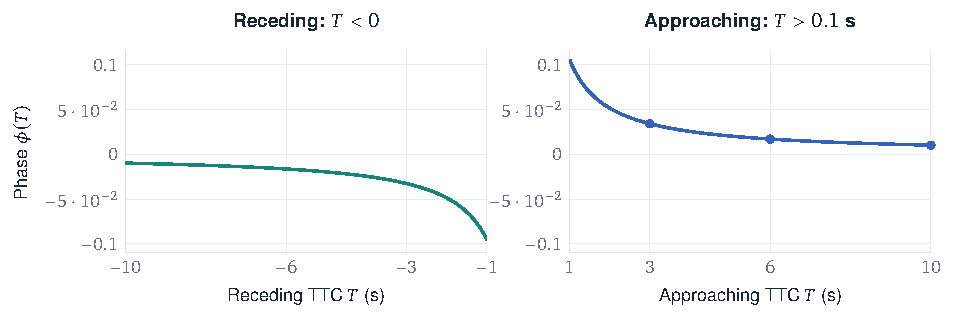
\includegraphics[width=\linewidth]{figures/rev_phase.pdf}
\caption{\textbf{Signed phase geometry.} Analytical curves show $|T|\in[1,10]$\,s on common vertical scales, with approaching-band markers at 3, 6, and 10\,s. The zoom excludes $[0,0.1]$\,s and the adjacent singularities.}
\label{fig:phase-geometry}
\end{figure}

The Simplex risk router selects among frozen expert TTCs by predicting relative expected absolute-phase costs. For three sorted expert phases, convexity and the 1-Lipschitz property of $\mathbb E|a-Y|$ imply ordered secant slopes $-1\leq s_0\leq s_1\leq1$. Softmax increments parameterize these constraints; integrating the slopes across expert-phase gaps yields relative costs. Hard selection returns one original expert prediction under a fixed tie order. The learned quantities are relative selection costs rather than calibrated collision probabilities. \evidence{M11}

The temporal refiner predicts a correction from a bounded feature history and four timing channels using a masked two-layer GRU; a causal Transformer provides the matched control. Histories require a contiguous valid suffix, and missing prefixes leave recurrent state unchanged. Residual mode anchors the phase at the median of the \emph{current} experts,
\begin{equation}
 \widehat\phi=\operatorname{median}(\phi_1,\phi_2,\phi_3)+0.03\,a_\theta(H).
\end{equation}
Separate heads predict phase-quantile widths and relative costs for the original experts; the latter do not estimate risk for the corrected output. Training combines phase absolute error, pinball losses, and relative-cost regression. Globally defined query mass supplies the weights without minibatch renormalization. Sparse-history variants retain selected slots from a longer history and recompute timing gaps from integer anchors, preserving cold starts and the original query population. \evidence{M12}

\subsection{Physical fields and temporal coordinates at the fusion interface}
\label{sec:physical-fusion-fields}
For each modality, the PHASE-ONLY input selects ten ordered fields from its context state: raw phase location (\texttt{raw\_location}), emitted point phase (\texttt{point\_phase}), the current A5, C2F, and PAIR expert phases, four current timing fields, and the number of valid history slots divided by eight. The twenty selected fields concatenate RGB first and events second. The first five fields are dimensionless signed-phase coordinates. The 160 learned hidden coordinates per modality are outside this input. Raw location precedes the native output guard, while emitted phase includes that guard. \evidence{M22,P04}

Let $a_j$ be the integer-microsecond anchor of retained observation $j$, $v_j$ its availability timestamp, and $q$ the current query. The four history timing fields, in order, are
\begin{equation}
 \left(\frac{a_q-a_j}{10^6},\quad
       \frac{v_q-v_j}{10^6},\quad
       \frac{a_j-a_{j^-}}{10^6},\quad
       \frac{v_j-a_j}{10^6}\right)\quad\mathrm{seconds}.
\end{equation}
The third field is zero for the first retained observation; missing prefixes are zero-padded and masked. Differences are formed as integers before conversion to seconds. The fusion interface takes the fields at the current slot, so its first two timing values are zero and its third describes the gap to the previous retained anchor. Availability denotes the latest admitted sensor or annotation dependency, not measured detector runtime; the final field is availability minus the observation's label anchor, without consuming a TTC value. \evidence{P04}

Context heads receive PHASE17 fields standardized by per-coordinate means and population standard deviations fitted on unique valid observations in the allowed fitting population; a standard deviation at most $10^{-6}$ is replaced by one. Padding remains zero. Their four timing channels are separate, expressed in seconds. At the subsequent PHASE-ONLY input, each modality's first five phase-valued fields are divided by $0.03$; the four timing fields remain in seconds and support remains valid-count$/8$. No fold-specific hidden-state standardization aligns latent coordinates. The RGB raw location also bypasses the correction MLP as its residual anchor, and the two native RGB width logits bypass it separately as quantile-width anchors. Zero correction therefore reproduces the RGB context prediction and widths. \evidence{M22,M23,P04}

\subsection{Observed field ranges and the event-history mismatch}
\label{sec:field-ranges}
Table~\ref{tab:field-ranges} lists the values that the timing and support fields take at the fusion input in three populations: the 88,744 out-of-fold TRAIN40 rows that fit the head, the 5,805 physical Test12 queries of the submission, and the 460 EvTTC transfer queries. The first, second, and fourth RGB timing fields and the second event timing field are zero everywhere. Raw location and emitted point phase coincide in 99.6\% of training rows and in all 460 transfer rows. On the transfer cohort the ten timing and support fields are constant or vary by less than $10^{-4}$, so the head acts there on the five phase values of each modality and, effectively, on four distinct values per modality.

\begin{table}[htbp]
\centering\small
\begin{tabular}{llll}
\toprule
Field & TRAIN40 out-of-fold & Test12 & EvTTC transfer \\
\midrule
RGB gap (s) & 0.1 (91\%), 0 (9\%) & 0.1 (96\%), 0 (4\%) & 0.1 \\
RGB valid slots / 8 & 0.625 (76\%), four other values & 0.625 (91\%), four other values & 0.625 \\
Event anchor offset (s) & 0.0009--0.020 & 0 & 0 \\
Event gap (s) & 0.05 (99.95\%), 0 & 0.1 (98\%), 0 (2\%) & 0.1 \\
Event valid slots / 8 & 0.875 (99.9\%) & 0.5 (95\%); never 0.875 & 0.5 \\
\bottomrule
\end{tabular}
\caption{Values of the non-constant timing and support fields at the fusion input. Training and Test12 values are computed from the archived out-of-fold features and staged submission features, which are outside the public source package; transfer values come from the released evaluation features.}
\label{tab:field-ranges}
\end{table}

The RGB fields have the same support in training and evaluation. The event fields do not. Training rows were generated with event-history slots every 50\,ms, all encoded inside the current query's object region; 99.9\% of rows have seven valid slots, a 0.05\,s gap, and an anchor-to-query offset between 1 and 20\,ms. Test12 and EvTTC inference instead assembled the event history from the observations of earlier queries, 0.1\,s apart, each encoded inside its own object region, giving a 0.1\,s gap, at most four valid slots, and zero offset. A gap of 0.1\,s and a support of 0.5 never occur in the training rows. The event context refiner, which receives the timing of all eight slots, and the fusion head were therefore evaluated outside their fitted support in these fields, and with history crops that follow the object instead of staying fixed in the query's frame.

This mismatch was identified after submission, by comparing archived inputs. Its effect on accuracy is unknown: the private Test12 labels are unavailable, and no local experiment has yet regenerated the event history at the training cadence. It is distinct from the PAIR interval normalization of Appendix~\ref{sec:canonical-cadence}, which concerns the duration fields of the pairwise readout. It may contribute to the absence of a measurable event benefit in Section~\ref{sec:design-analysis}, and it means the benchmark score was obtained with a degraded event path.

\subsection{Multimodal complement and uncertainty boundaries}
The later joint-measurement complement anchors on RGB phase and learns a correction from RGB features, event features, and the RGB phase itself:
\begin{equation}
 \widehat\phi=\phi_{\mathrm{RGB}}+s\,g_\theta
   ([z_{\mathrm{RGB}},z_{\mathrm{event}},\phi_{\mathrm{RGB}}]).
\end{equation}
The final layer starts at zero, so the initial prediction reproduces the RGB anchor up to native phase conversion. A matched ZERO control removes the complete event-feature block, including admitted event-clock features, while retaining network capacity. When RGB is absent, the model copies the event TTC without applying correction or averaging. The paired TRUE--ZERO comparison isolates the contribution of event information to the learned RGB correction. \evidence{M13}

Uncertainty has multiple meanings across these families. The causal-scale route predicts log-variance in log-ratio space and propagates it through the local Jacobian. For $q=\operatorname{expm1}(r)/\Delta t$,
\begin{equation}
 \operatorname{Var}(q)\approx \frac{e^{2r}}{\Delta t^2}\operatorname{Var}(r),\qquad
 \operatorname{Var}(T)\approx \frac{\Delta t^2e^{2r}}{(e^r-1)^4}\operatorname{Var}(r).
\end{equation}
The singularity near zero expansion requires separate finite-output and \texttt{known} indicators. The implementation marks unsupported or near-zero log-ratio predictions unknown and derives model-based threshold probabilities from an inverse-TTC Gaussian approximation. Empirical calibration requires measurements of coverage, calibration error, and corruption response. The temporal refiner's phase quantiles carry a different meaning from collision-class probabilities. \evidence{M07,M12}

\subsection{Optimization and execution semantics}
Component losses keep their true counts over each effective batch, and tail top-$k$ selection uses the complete effective batch instead of separate microbatches. Activation recomputation preserves random-number-generator state, keeping gradient accumulation and recomputation equivalent to the stated objective. The joint-measurement loss includes teacher relations, unlike the label-free JEPA loss. \evidence{M14}

Deployment optimizations include bounded event history, chunked memory, persistent input state, reusable feature caches, and graph execution. Because each changes state lifetime, numerical-parity tests accompany every admitted path. Runtime measurements state the associated preprocessing and inference boundary.

\section{Evaluation details and causal checks}
\label{app:evaluation-details}
This appendix describes data separation, causal checks, and runtime measurement in detail.

\subsection{The unit of independence}
Windows from one trajectory share appearance, geometry, object identity, and adjacent event history. Complete sequence groups define the grouped partitions, while the resampling unit depends on the study. Public metadata establish separation by sequence identifier but do not establish independent physical acquisition sessions for every distinct identifier. Small disjoint splits remain development evidence when the project has reused their sequences for diagnosis. This limitation does not itself demonstrate leakage. \evidence{M16,M23,P02}

The corrected grouped-recovery protocol keeps learned parents fold-local. Outer-development rows are excluded from encoder fitting, teacher-target retrieval for training, training losses, fitted feature statistics, and expert-parent fitting. A shared immutable DINO teacher cache may contain rows that a fold never retrieves. Cache storage and fold-specific consumption therefore have different boundaries. A frozen parent still carries its prior exposure, so the analysis follows sample membership through preprocessing, checkpoints, retrieved targets, normalization, and model selection. \evidence{P02}

A deterministic event representation can be reused when preprocessing and sample identity stay fixed. A checkpoint fitted on a larger population changes the exposure of every downstream result. File identity verifies which representation or model was used; training membership determines the strength of the resulting claim. \evidence{M17}

\subsection{Study-specific paired inference}
Historical V5 outer-development and V7 comparisons use 422 clusters, each defined by a sequence identifier and a track identifier. They use 5,000 paired bootstrap replicates over 8,192 queries from nine sequences. Their seed-7 fits do not replicate representation training across seeds. The earlier public-validation paired audit instead uses 108 sequence--track clusters over 2,048 queries. These historical intervals retain their original units even when the reported point metric averages sequences. \evidence{P02}

Table~\ref{tab:audit-bootstrap-units} distinguishes these intervals from the later sequence and hierarchical analyses. The source protocol's occasional label ``acquisition group'' denotes the recorded sequence grouping; independence between physical acquisition sessions remains unverified.
\begin{table}[H]
\centering\scriptsize
\caption{Resampling units for selected paired analyses. Counts describe the recorded protocols, not independent acquisitions or independent pretraining runs. Archived numerical intervals are unchanged. \evidence{P02,L03,N02,R01,A02--A04,H_V16}}
\label{tab:audit-bootstrap-units}
\begin{tabularx}{\linewidth}{@{}p{.20\linewidth}p{.23\linewidth}p{.15\linewidth}X@{}}
\toprule
Study & Resampling unit & Replicates & Seeds and reduction \\
\midrule
Public-validation paired audit & 108 sequence--track clusters; 2,048 rows & 5,000 & Fixed fitted checkpoints; paired rows, sequence-macro MiD. \\
V5--V7 grouped development & 422 sequence--track clusters; nine sequences, 8,192 rows & 5,000 & Seed-7 models; bootstrap seed 20260813. Seeds are not extra clusters. \\
V12 H16--H8 replication & Nine sequences, then tracks within sampled sequences & 8,192 accepted hierarchical draws & Per-query losses averaged across fixed matched head seeds; separate exact sequence comparison. \\
V16 PHASE-ONLY selection & Eight V sequence groups & 4,000 & Bootstrap seed 20261012; group-macro bucket MiD contrasts separately for head seeds 7/13/23. \\
V18 TRUE/ZERO fusion & Eight V sequence groups & 2,000 & Bootstrap seed 12345; groupwise MiD averaged over fixed seeds 7/13/23; no TTC ensembling. \\
Grouped F1 adaptation & Seven scenario families; 24 recordings & 2,000 & Bootstrap seed 7; recording-macro RAE differences separately for head seeds 7/13/21. \\
401-parameter gate confirmation & Four CCRm recordings within one family & 2,000 & Bootstrap seed 7; query-weighted RAE difference for the fixed three-seed ensemble. \\
Startup router comparison & Five road scenario families & 5,000 & Bootstrap seed 7; query-weighted RAE differences for fixed three-seed ensembles. \\
Historical Extended-new snapshot & 32 complete sequence groups; 468 eligible rows under the former target map & 10,000 & Seed 20261028; pooled-query mean, median, and p95; superseded target assignment. \\
Corrected Extended-new analysis & 32 complete sequence groups; 460 eligible rows after target reassignment & 10,000 & Seed 20261028; paired saved predictions and corrected eligibility; no model refit. \\
Canonical cadence & 24 road recordings; Slider-500 separate & 10,000 & Seed 7; recording-macro differences. One Slider recording has no between-recording interval. \\
Later JEPA pilot closure & Eight complete sequence groups & Not recorded in the distributed summary & Seeds 7/13/21 kept together; descriptive post hoc sequence intervals. \\
\bottomrule
\end{tabularx}
\end{table}


Comparisons pair the same eligible rows and sequences. For per-row metric differences $d_{si}$ in sequence $s$, the sample-weighted estimate is
\begin{equation}
 \widehat\Delta=\frac{\sum_s\sum_{i=1}^{n_s}d_{si}}{\sum_s n_s}.
\end{equation}
A paired sequence bootstrap samples sequence identities with replacement and carries every row from each selected sequence into the replicate. Sample-weighted resampling recomputes the ratio of summed differences to summed counts; the sequence-macro calculation averages sequence means. The scorer-wrapper comparison uses the sample-weighted form with a fixed bootstrap seed, complete sequence clusters, and no removal of invalid MiD rows. This wrapper does not redefine the historical recovery bootstraps. \evidence{M15}

Intervals based on few sequences have limited precision and inherit development exposure and experiment multiplicity. Random seeds measure optimization variation for a fixed split, whereas out-of-fold partitions vary the held-out groups. Results report seeds, folds, and sequences separately.

\subsection{Causality tests}
Prefix-invariance tests determine whether later inputs alter an earlier output. The causal-scale suite checks foreground logits, geometry tokens, pair tokens, analytic and residual log-ratios, and TTC. A legacy symmetric smoother provides a positive control by violating prefix invariance; the causal-left mode must remain invariant under the same perturbation. \evidence{M18}

Network masks alone cannot establish causality. Tests also perturb crop coordinates, normalization inputs, teacher frames, and labels. Self-supervised samples must remain unchanged when labels change, and crop tests restrict geometry to the designated endpoint boxes.

Streaming tests cover state reset and update semantics. The bounded object-ROI estimator rejects timestamp rollback until reset, validates aligned packets and coordinates, and discards events outside its history. It consumes ROI-local event coordinates and supplied object observations. Paced replay then adds acquisition, queuing, temporal state, multiple objects, and host-visible output. \evidence{M03,M18,M19}

\subsection{Matched controls and the scope of attribution}
Architectural ablations match rows, seeds, training budgets, parent exposure, selection rules, and model capacity. A zeroed-input model removes modality information while retaining capacity. A shuffled-future control disrupts temporal correspondence while preserving the future marginal and optimization schedule. A frozen random encoder measures what the downstream head can recover without learned features.

A hard router selects among fixed expert predictions; a residual phase model can correct them. Teacher distillation measures the effect of privileged RGB supervision on an event backbone. Failed and vetoed arms remain in the analysis because they constrain mechanism-level explanations.

\subsection{Latency, memory, and sustained service}
A tensor-forward benchmark starts after tensor preparation. The paced runner instead includes a RAW producer, absolute arrivals, a bounded queue, and host-visible output. Completion occurs when the consumer returns every required prediction. Fixed arrivals expose backlog, while the results record drops, acquisition errors, incomplete histories, and invalid outputs. \evidence{M20}

The primary deadline-to-output response is
\begin{equation}
 L_i=t_i^{\mathrm{host\ output}}-t_i^{\mathrm{scheduled\ arrival}}.
\end{equation}
A secondary clock starts after RAW acquisition. Deadline evaluation reports tail quantiles, maximum response, coverage, backlog, and drops because mean response can hide missed arrivals. Warmup uses data available before the first admitted anchor. The 50-Hz milestone requires sustained cadence, numerical parity, and complete finite outputs. \evidence{M20}

The available RAW sequences are shorter than the sustained-service milestone. The replay therefore characterizes short-run latency for its hardware, population, numerical tolerance, and duration.

Implementation checks and their scope are reported in Appendix~\ref{app:reproduction}. The official leaderboard score evaluates prediction accuracy; it provides no measurement of sensor-to-output latency or sustained service. \evidence{M21}

\clearpage
\section{Paired transfer uncertainty and numerical cases}
\label{app:derived-transfer}
I analyze the saved query-level predictions in \path{data/transfer_queries.csv} (L46). Source key R01 maps the derived results to \path{revision/derived_transfer_analysis.json}; \path{scripts/prepare_revision.py} regenerates them.

\subsection{Exact paired sequence bootstrap}
The analysis uses the 468 eligible Extended-new predictions and their 32 physical-sequence groups. Each of 10,000 replicates samples 32 group identities with replacement and includes every query from each sampled group. Repeated groups contribute repeated queries. PHASE-TTC and RGB share the sampled indices. For each model, I compute pooled mean, median, and 95th-percentile absolute error, then form the PHASE-minus-RGB difference. NumPy's \texttt{linear} quantile convention and \texttt{default\_rng(20261028)} define the 2.5th and 97.5th percentile endpoints.

The point differences are \RevisionMeanDelta\,s for the mean, \RevisionMedianDelta\,s for the median, and \RevisionPninetyfiveDelta\,s for p95. All three intervals contain zero (Table~\ref{tab:revision-bootstrap}). The exploratory intervals condition on the fitted models and development-exposed sequences; they do not incorporate representation-training variability or adaptive model selection.

Differences use full-precision predictions. The mean difference rounds to $+0.007$\,s; subtracting the separately rounded means 1.023 and 1.015 instead gives $+0.008$\,s.

\subsection{Numerical cases}
The two queries below maximize and minimize the PHASE-minus-RGB absolute-error difference within the saved predictions. These post hoc examples show the range of model disagreement; their causes would require inspection of the corresponding sensor observations.
\begin{table}[H]\centering\small
\caption{Queries with the largest positive and negative PHASE-minus-RGB absolute-error differences in the labeled transfer set. \evidence{R01,L46}}
\label{tab:revision-cases}
\begin{tabularx}{\linewidth}{@{}Xrrrr@{}}\toprule
Query & Target (s) & PHASE (s) & RGB (s) & $\Delta$ AE (s)\\\midrule
{\footnotesize\path{CPNAO-high:13700430}} & 2.996 & 6.604 & -12.903 & -12.290\\
{\footnotesize\path{CCRs-1-medium-100-overlap-100:5950352}} & 6.765 & -25.740 & -9.880 & +15.861\\
\bottomrule\end{tabularx}\end{table}
\FloatBarrier

\clearpage
\subsection{Complete sequence comparisons}
\begin{figure}[H]
\centering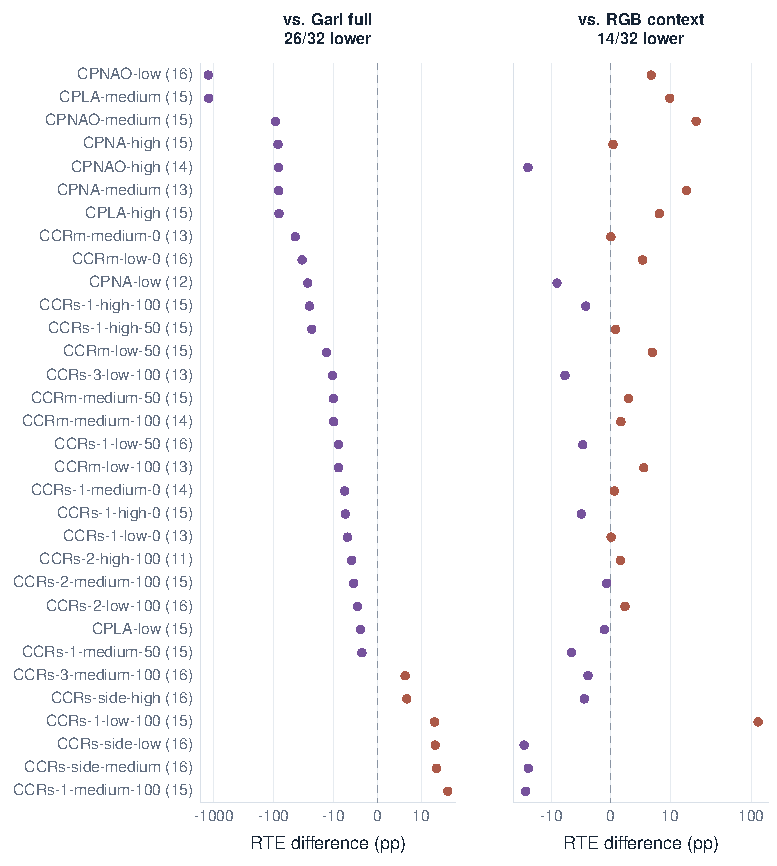
\includegraphics[width=\linewidth,height=.70\textheight,keepaspectratio]{figures/rev_sequence.pdf}
\caption{\textbf{Sequence-level relative TTC error differences.} Both panels show the 32 labeled Extended-new sequences in a common order; parentheses give query counts and negative values favor PHASE-TTC. The symmetric-log axes are linear between $-5$ and $+5$ percentage points. Display labels omit repeated overlap suffixes; Table~\ref{tab:sequence-full} gives the full identities. \evidence{R01,L46}}
\label{fig:transfer-sequence}
\end{figure}
\FloatBarrier
\clearpage
{\small\begin{longtable}{@{}p{6.0cm}rrrrr@{}}
\caption{Query counts and mean RTE (\%) for all 32 Extended-new sequences. Differences are in percentage points. \evidence{R01,L46}}\label{tab:sequence-full}\\
\toprule Sequence & $n$ & PHASE & RGB & Garl & $\Delta_{\rm RGB}$\\\midrule\endfirsthead
\toprule Sequence & $n$ & PHASE & RGB & Garl & $\Delta_{\rm RGB}$\\\midrule\endhead
\bottomrule\endfoot
CPNAO-low & 16 & 46.95 & 41.09 & 1283.26 & +5.86\\
CPLA-medium & 15 & 45.43 & 35.53 & 1265.98 & +9.90\\
CPNAO-medium & 15 & 41.92 & 20.94 & 134.36 & +20.98\\
CPNA-high & 15 & 66.50 & 66.14 & 150.71 & +0.36\\
CPNAO-high & 14 & 55.86 & 75.18 & 137.89 & -19.31\\
CPNA-medium & 13 & 59.61 & 43.68 & 141.20 & +15.93\\
CPLA-high & 15 & 62.29 & 54.92 & 143.22 & +7.37\\
CCRm-medium-0-overlap-0 & 13 & 14.61 & 14.57 & 57.78 & +0.04\\
CCRm-low-0-overlap-0 & 16 & 16.40 & 11.85 & 49.69 & +4.56\\
CPNA-low & 12 & 35.90 & 44.34 & 62.54 & -8.44\\
CCRs-1-high-100-overlap-100 & 15 & 19.23 & 22.75 & 44.19 & -3.52\\
CCRs-1-high-50-overlap-50 & 15 & 18.25 & 17.55 & 41.09 & +0.71\\
CCRm-low-50-overlap-50 & 15 & 17.70 & 11.67 & 30.65 & +6.02\\
CCRs-3-low-100-overlap-100 & 13 & 8.35 & 15.08 & 18.67 & -6.73\\
CCRm-medium-50-overlap-50 & 15 & 20.93 & 18.41 & 30.93 & +2.53\\
CCRm-medium-100-overlap-100 & 14 & 15.25 & 13.79 & 25.04 & +1.47\\
CCRs-1-low-50-overlap-50 & 16 & 4.98 & 8.93 & 13.15 & -3.95\\
CCRm-low-100-overlap-100 & 13 & 20.69 & 15.96 & 28.85 & +4.73\\
CCRs-1-medium-0-overlap-0 & 14 & 6.72 & 6.17 & 13.14 & +0.55\\
CCRs-1-high-0-overlap-0 & 15 & 17.32 & 21.49 & 23.61 & -4.17\\
CCRs-1-low-0-overlap-0 & 13 & 9.81 & 9.73 & 15.58 & +0.07\\
CCRs-2-high-100-overlap-100 & 11 & 13.75 & 12.35 & 18.65 & +1.40\\
CCRs-2-medium-100-overlap-100 & 15 & 6.84 & 7.39 & 11.36 & -0.55\\
CCRs-2-low-100-overlap-100 & 16 & 15.67 & 13.62 & 19.44 & +2.05\\
CPLA-low & 15 & 25.19 & 26.09 & 28.38 & -0.90\\
CCRs-1-medium-50-overlap-50 & 15 & 5.73 & 11.32 & 8.66 & -5.60\\
CCRs-3-medium-100-overlap-100 & 16 & 15.32 & 18.54 & 9.91 & -3.21\\
CCRs-side-high & 16 & 21.54 & 25.26 & 15.77 & -3.72\\
CCRs-1-low-100-overlap-100 & 15 & 395.63 & 273.53 & 378.78 & +122.10\\
CCRs-side-low & 16 & 41.76 & 63.28 & 24.48 & -21.52\\
CCRs-side-medium & 16 & 46.06 & 65.11 & 27.92 & -19.05\\
CCRs-1-medium-100-overlap-100 & 15 & 111.28 & 131.87 & 83.19 & -20.60\\
\end{longtable}}


\section{Competition adaptation and complete prediction traces}
\label{app:competition-details}
This appendix details input construction and timing for the original 434-query competition inference snapshot of 28 October. Linear and symmetric-log views show the full signed prediction traces. The corrected target audit and quality-adapted PHASE-TTC comparison added on 1 November appear in Section~\ref{sec:quality-adaptation}; they do not alter the frozen predictions shown here. \evidence{T01,N01}

\subsection{Frozen models and causal input construction}

I use the public Hugging Face full, event-only, and visual-only checkpoints with their released configurations and source revision. Strict state-dictionary loading and float32 inference keep each model fixed. The release identifies the checkpoint bytes but does not document complete training membership, so the evaluation represents frozen-checkpoint adaptation rather than a claim of clean zero-shot transfer.

Garl-TTC predicts the ratio of object heights at two endpoints and converts it to TTC as
\begin{equation}
 \widehat T
 =\frac{\Delta t_{\mathrm{measured}}}
 {1-\widehat h_0/\widehat h_1}.
 \label{eq:garl-height-ratio-evttc}
\end{equation}
The released configuration sets the native model field $\mathrm{dT}=0.1$\,s. For Equation~\ref{eq:garl-height-ratio-evttc}, the adapter substitutes the measured separation of each endpoint pair while leaving the released representation unchanged. The checkpoint metadata do not establish the cadence used during training.

The full and visual routes select the latest real RGB frame at or before a query, then the preceding frame closest to 100\,ms earlier. Full Garl builds one causal event window per RGB endpoint with support capped at $\min(\Delta t_{\mathrm{measured}},100\,\mathrm{ms})$. Event-only Garl uses two consecutive 100\,ms windows after startup and splits the observed causal prefix into two intervals for earlier queries. Each endpoint uses the released 20-plane, polarity-agnostic time volume. Queries without sufficient history remain gaps.

PHASE-TTC uses its declared 650\,ms causal history. The shared query population therefore compares the frozen systems under their respective temporal support.

Supplied boxes use zero-based, half-open event-plane coordinates. The adapter selects the latest box available at each endpoint; if the endpoint precedes all query-causal boxes, it uses the earliest such box and records availability at query time. Road sequences pair right Blackfly RGB with right Prophesee events. Slider uses its supplied streams and a rotation derived from camera poses because its calibration lacks a named event-to-RGB extrinsic. Calibrated intrinsics, distortion, and rotation-only ray projection map the event box into RGB; unavailable object depth precludes translational correction. A common square edge spans the endpoint boxes, with endpoint-specific event centers and the current center applied to both RGB frames.


\subsection{Published three-sequence comparison}
Table~VI of the eAP paper reports Garl-TTC on three EvTTC sequences, with an unweighted mean RTE of 10.60\% \citep{eap}. That study uses a separate labeled population; shared scenario names do not establish shared recordings or query identities. \evidence{T02}
\begin{table}[H]
\centering\small
\caption{Garl-TTC's published zero-shot relative TTC error on three EvTTC sequences, as reported in the eAP paper, Table VI. \evidence{T02}}
\label{tab:evttc-published-rte}
\begin{tabular}{@{}lr@{}}
\toprule
\textbf{Published sequence} & \textbf{RTE (\%)} \\
\midrule
CCRs2-medium & 8.31 \\
CCRs2-high & 10.56 \\
CCRm-medium & 12.93 \\
\textbf{Unweighted average} & \textbf{10.60} \\
\bottomrule
\end{tabular}
\end{table}

\begin{table}[H]
\centering\scriptsize
\caption{Garl--PHASE prediction comparisons for all ten sequences. Each entry gives shared-finite coverage and median absolute prediction difference in seconds. \evidence{T01}}
\label{tab:evttc-sequence-disagreement}
\setlength{\tabcolsep}{3.2pt}
\begin{tabular}{@{}lrrr@{}}
\toprule
\textbf{Sequence} & \textbf{Full $n/N$; med.} & \textbf{Event $n/N$; med.} & \textbf{Visual $n/N$; med.} \\
\midrule
CCRs1-low & 49/50; 0.465 & 50/50; 0.776 & 49/50; 0.213 \\
CCRs1-medium & 42/43; 0.308 & 43/43; 0.863 & 42/43; 0.200 \\
CCRs1-high & 29/30; 0.207 & 30/30; 0.519 & 29/30; 0.111 \\
CCRs2-low & 45/46; 0.221 & 46/46; 0.339 & 45/46; 0.243 \\
CCRs2-medium & 54/55; 0.178 & 55/55; 1.045 & 54/55; 0.254 \\
CCRs2-high & 58/59; 0.188 & 59/59; 0.682 & 58/59; 0.223 \\
CCRm-low & 41/42; 0.270 & 42/42; 0.703 & 41/42; 0.283 \\
CCRm-medium & 39/40; 0.151 & 40/40; 0.839 & 39/40; 0.350 \\
Slider-750 & 49/51; 0.408 & 51/51; 0.470 & 51/51; 0.258 \\
Slider-1000 & 18/18; 0.288 & 18/18; 0.119 & 18/18; 0.067 \\
\bottomrule
\end{tabular}
\end{table}


\subsection{Runtime boundary and interpretation}

\begin{table}[H]
\centering\small
\caption{Offline processing time in seconds per query. Model time covers the synchronized forward pass and host output; full time includes tensor preparation. The Garl variants ran in full/event/visual order; PHASE-TTC used its own adapter and history length. \evidence{T01}}
\label{tab:evttc-runtime}
\begin{tabular}{@{}lrrrr@{}}
\toprule
\textbf{Model} & \textbf{Model med.} & \textbf{Model P95} & \textbf{Full med.} & \textbf{Full P95} \\
\midrule
PHASE-TTC & 0.753 & 7.820 & 2.687 & 9.073 \\
Garl full & 0.039 & 0.045 & 0.542 & 1.009 \\
Garl event-only & 0.007 & 0.011 & 0.350 & 0.806 \\
Garl visual-only & 0.007 & 0.011 & 0.158 & 0.221 \\
\bottomrule
\end{tabular}
\end{table}


Timing separates tensor preparation from the synchronized model-to-host call and excludes loading, indexing, calibration, source hashing, and result serialization. The variants run once in full, event-only, visual-only order, so operating-system and HDF5 caches and GPU warm state can carry between runs. Table~\ref{tab:evttc-runtime} reports these observations alongside PHASE-TTC, whose adapter and temporal support differ.

Independent verification accounts for each planned record and replays the float32 height-to-TTC conversion. Full and visual Garl remain partial because of input gaps; event-only contains all 434 rows. Across the ten sequences, the four routes exhibit distinct signed behavior and disagreement tails. \evidence{T01}

\subsection{Target audit and evaluation boundary}
The later audit recovers all 434 local TTC targets after correcting the public source mapping for CCRs1-low and CCRs1-medium. It preserves the recorded clock offsets rather than fitting timing shifts to match errors. Earlier 423-target summaries are superseded. The corrected original-versus-adapted comparison applies the same documented handling of negative predictions to both columns and reports complete population counts. The historical signed traces below retain their original values and gaps. \evidence{N01}

For Slider-750, the corrected local evaluator gives 283.931058\% relative error for the original PHASE-TTC predictions, compared with 132\% in the organizer-provided result. The other nine rows agree after rounding. The adapted local value of 76.071442\% therefore cannot be compared directly against the organizer's 132\% as if both used an equivalent scoring contract. The unresolved target/evaluator correspondence and the cohort's historical development exposure remain explicit limitations. This appendix supplies no new error ranking for the three Garl variants. \evidence{N01}

\clearpage
\subsection{All ten sequences, with missing inputs preserved}
\begin{figure}[H]
\centering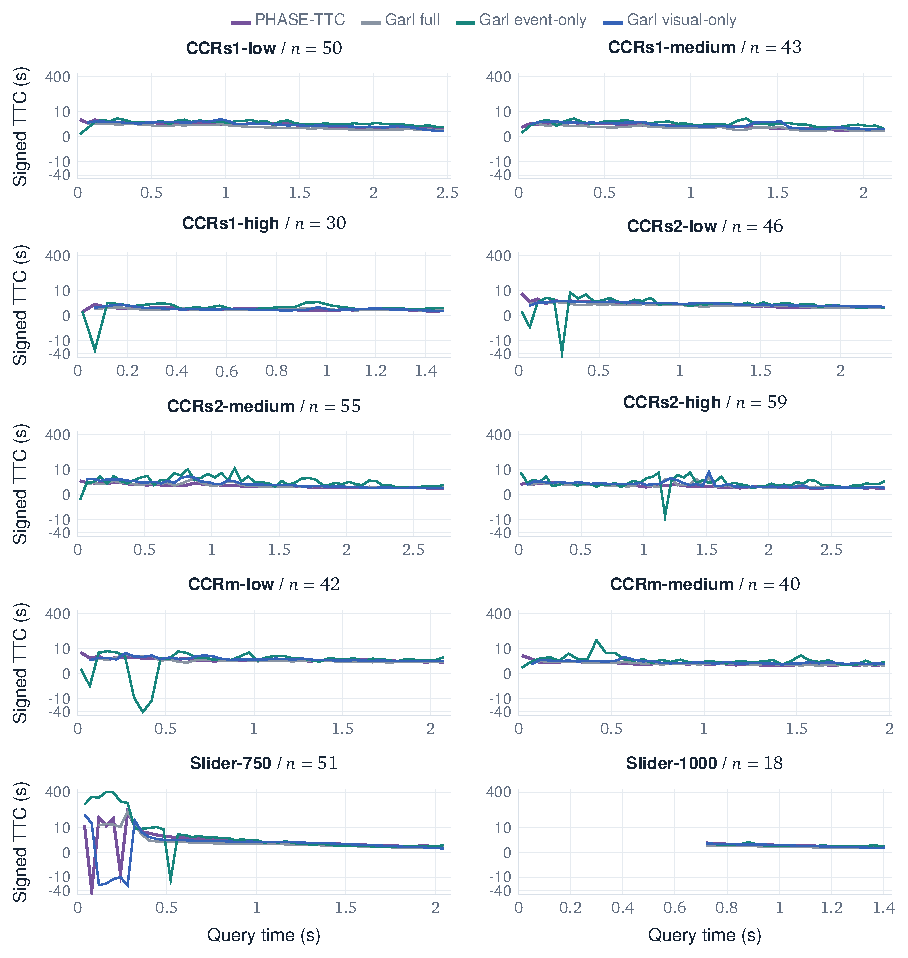
\includegraphics[width=\linewidth,height=.72\textheight,keepaspectratio]{figures/rev_competition_symlog.pdf}
\caption{\textbf{Signed predictions on a symmetric-log scale.} PHASE-TTC is purple, Garl full gray, event-only teal, and visual-only blue. All panels are linear inside $[-2,2]$\,s and logarithmic outside; gaps mark unavailable inputs. \evidence{T01}}
\label{fig:evttc-predictions-symlog}
\end{figure}
\clearpage
\begin{figure}[H]
\centering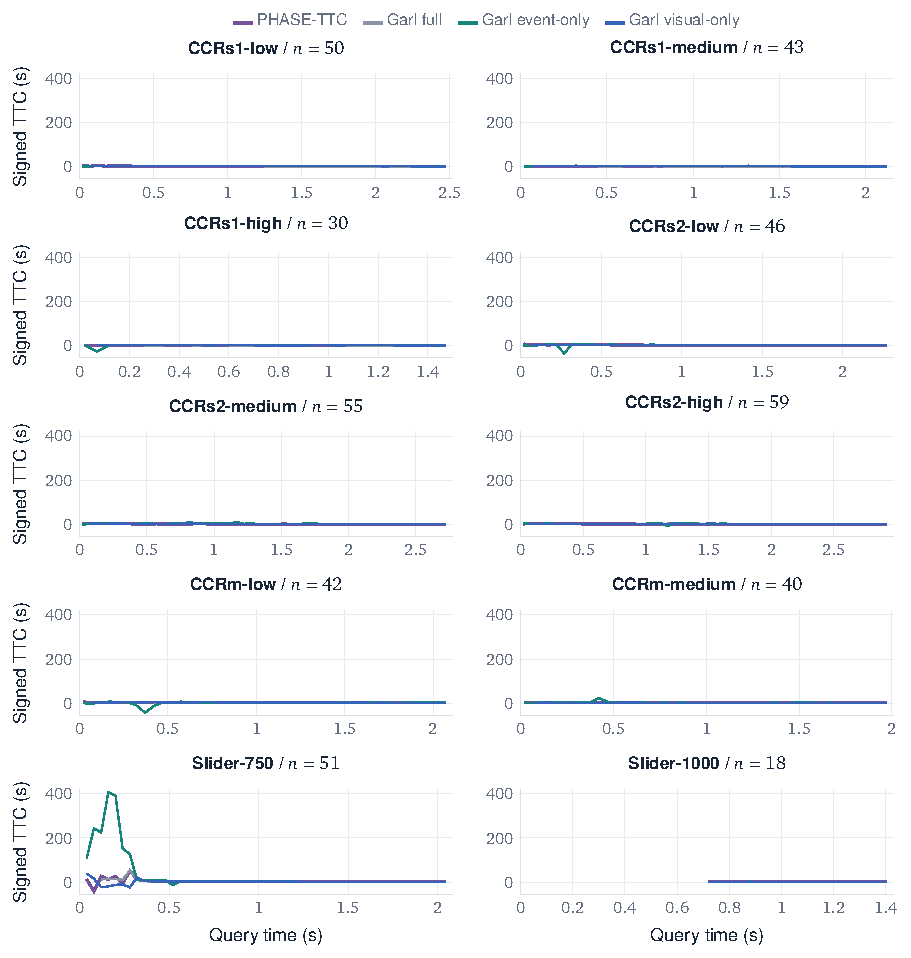
\includegraphics[width=\linewidth,height=.72\textheight,keepaspectratio]{figures/rev_competition_linear.pdf}
\caption{\textbf{Signed predictions on a common linear scale.} The same outputs as Figure~\ref{fig:evttc-predictions-symlog} show the full excursion range, which compresses the central values. \evidence{T01}}
\label{fig:evttc-predictions-linear}
\end{figure}
\FloatBarrier

\clearpage

\section{Historical design analysis and controlled ablations}
\label{app:design-history}
Three findings shaped PHASE-TTC: preserving scale change mattered more than representation stability alone; correcting an expert's phase could improve on selecting an expert; and changing the loss often traded one TTC range against another. The studies below used different data splits and pretrained models. Appendices~\ref{sec:early}, \ref{sec:temporal-recovery}, and~\ref{sec:late} give the full configurations and unsuccessful variants.

\subsection{Preserve the motion variable before predicting it}
Using a common object region preserves apparent expansion across observations. Independently resizing each endpoint can remove that signal before the network sees it (Figure~\ref{fig:crop}). An explicit object query also distinguishes objects that share one full-frame input but have different TTC targets. The estimator consequently requires externally supplied localization. \evidence{M03}

The geometry experiments exposed a related difficulty: stable foreground maps and accurate absolute heights did not ensure accurate changes in scale. Some models also received RGB-derived SAM masks or DINOv3 relations during training, even when their inference inputs contained only events.

Removing paths from a trained V8 model identified which inputs its prediction used. Analytic scale alone scored 373.18 MiD, and adding the residual without transport gave 373.60. Restoring transport reduced the score to 163.23; restoring history reduced it further to 155.82. The weights remained fixed throughout these tests. \evidence{E02,E12,E25,E26,E21,E23,E24}

\subsection{Predictive embeddings and dynamic scale}
Predicting a future embedding and estimating expansion are different objectives. A representation can make the future easy to predict by retaining persistent appearance, yet discard the small changes needed to recover $\dot s/s$. Conversely, preventing collapse by maintaining variance says little about which physical variable supplies that variance. This distinction motivates evaluating TTC and geometric increments alongside prediction loss.

In the synthetic controls, a temporal-residual objective recovered more dynamics than variance regularization when nuisance features changed slowly. Making those nuisances vary independently across frames reversed the ordering. By varying nuisance dynamics independently of the target motion, this controlled construction shows how the choice of predictable signal changes the ordering of the objectives, consistent with the slow-feature concern raised by \citet{slowfeatures}. Testing that mechanism on real driving data requires interventions on the nuisance signal. \evidence{E02,E12}

On real data, the V8 frozen and partially fine-tuned JEPA encoders failed the benefit criterion against scratch, random-frozen, and shuffled-future controls. A separate fixed-teacher pilot reduced future-state loss while worsening teacher-increment loss and failed to outperform both static and shuffled-future controls on annotated log-height change. Across these tests, predictive pretraining fell short of the prescribed benefit criteria. The role of background appearance in the real-data result is an open attribution question. Appendices~\ref{sec:early}, \ref{sec:methods}, and~\ref{app:physics-followup} give the objective definitions and controls. \evidence{E23,E24,N04}

These findings motivate measuring expansion directly at the fusion interface and checking it at the TTC output. They leave open whether other predictive targets, sampling schemes, or training budgets can learn a better motion representation.

\subsection{Correct phase rather than only selecting an expert}
A hard router is limited to the predictions its experts already make. SIMPLEX-T can move beyond them by learning a correction around their median phase from masked temporal context. The auxiliary cost head describes the original experts; evaluating the corrected prediction's risk requires a corresponding risk target. Phase quantiles also need empirical calibration before use as collision probabilities. \evidence{M_TEMPORAL_MODEL,M_PHASE_CONTRACT}

Extending the context from eight history slots (H8) to sixteen (H16) lowered MiD for each of three head seeds on the initial exploration cohort. The paired interval across all seeds excludes zero. However, one seed had already informed exploration; the two new seeds alone give a difference of $-2.42$ MiD with interval $[-5.24,0.04]$. All heads shared the same upstream producers. Figure~\ref{fig:middle-h16} shows both summaries; H8 remained the selected candidate. \evidence{M_SIMPLEX}


Keeping all experts produced the lowest score in the removal study: FULL-C0 reached 121.40 MiD, compared with 127.79 for A5-only, 126.70 for C2F-only, and 124.67 for A5 plus PAIR.

In the temporal-aggregation comparison, set aggregation with age gave 122.44 MiD; removing explicit time gave 123.69. Because the frozen experts can already encode temporal information, the remaining differences cannot be assigned to recurrence alone.

Transport probes improved on destructive controls, but stronger calibrated or pooled alternatives narrowed that advantage. \evidence{M_SIMPLEX,M_STAGE61,M_STAGE62}

\subsection{Adaptation trades error between TTC ranges}
Changes to the readout often improved imminent-contact estimates at the expense of receding motion. The band-reweighted phase-loss arm (V14 M1--L0) reduced crucial MiD from 156.83 to 134.47 but increased negative MiD from 61.38 to 84.21. V17's geometry bypass lowered the aggregate score on the development-used V split from 106.545 to 102.762 while worsening MAE; its head seeds shared encoders. Across V14--V17, loss reweighting, residual range, sampling, numerical precision, clipping, geometry bypasses, and height readouts failed to meet all acceptance criteria. Invalid height-derived predictions were retained in scoring. The next experiments therefore allowed the measurement model itself to adapt. \evidence{L02,L50--L52}

V18 full adaptation reduced aggregate MiD on H from 112.29 to 78.92 and crucial MiD from 157.27 to 95.85, while negative MiD rose from 65.52 to 87.09. The model passed the overall sign criterion but remained inaccurate in the magnitude of receding TTC. V19 increased the training weight on negative targets and recovered some negative-range accuracy and MAE, at the cost of aggregate and crucial-range error. \evidence{L10,L24,L25,L30}

\subsection{Events help in the matched V18 comparison}
Supplying real events improved V18 C1 relative to its equal-capacity ZERO control. TRUE-event fusion achieved aggregate MiD $87.29\pm0.87$, compared with $92.47\pm0.16$; dispersion is the sample standard deviation of the scalar scores across seeds. The paired comparison over complete groups also favored TRUE. Each seed repeated C1 adaptation and head fitting from the same A5 initialization and RGB context model. This experiment uses V18 C1, whereas the final forty-sequence system derives from V16. \evidence{L03,L31--L33}


Section~\ref{sec:v16-selection} separates the historical V16 selection and its four-fold context cross-fit from the later five-rotation TRAIN40 refit. The V18 crucial-band gain remained below its registered threshold. Its comparison with the preserved V16 model gave an interval of approximately $[-3.69,0.14]$, and no V18 candidate met all acceptance criteria. Section~\ref{sec:design-analysis} reports new equal-capacity final-head controls on fixed source-domain out-of-fold features. Those controls keep the temporal support of the final refiners; they do not compare against retrained Garl producers.
\FloatBarrier

\section{Geometric adapter implementation and earlier evaluation}
\label{app:quality-complete}
\cohortline{LOCAL ADAPTATION / 2,608 fitting queries / 434 corrected evaluation queries / historical exposure retained}

The base fusion model supplies several estimates of the same signed quantity: its final fused TTC, the RGB context estimate, and the event context estimate. Their errors need not agree, and their reliability changes with temporal support and apparent motion. PHASE-TTC-Adapt leaves all nine upstream components frozen and learns a small router over those three outputs and a causal box-expansion estimate. The experiment adapts the fusion rule over fixed representations; Section~\ref{sec:canonical-cadence} evaluates temporal normalization as a separate intervention. \evidence{N01}

The adapter uses the frozen base model, denoted F0 in the source archive. Earlier fine-tuned heads and quality-gate candidates are separate models; Appendix~\ref{app:adaptation-lineage} documents their populations, unsuccessful controls, and interval coverage. In particular, the delivered router does not use the fine-tuned weights affected by the earlier target-source assignment.

\subsection{Causal box geometry and its quality descriptors}
For each query, the geometric branch admits supplied boxes with timestamps in the preceding 650\,ms, rejects nonfinite or nonpositive extents, and requires strictly increasing observation times. It fits three apparent sizes: width, height, and square root of area. Let $s_i$ denote one such size, $s_n$ its latest value, and $u_i$ time relative to the query in seconds. The branch constructs $\rho_i=s_n/s_i$ and estimates a line using median pair slopes,
\begin{align}
 b &= \operatorname{median}_{i<j}\frac{\rho_j-\rho_i}{u_j-u_i},
 &a &= \operatorname{median}_i(\rho_i-bu_i),\\
 q_s&=-b/a \quad (a>0).
\end{align}
The median of the three $q_s$ values supplies the geometric inverse TTC. This is an apparent-scale model with a query-time intercept; it does not recover metric depth or compensate for arbitrary rotation, occlusion, or annotation jitter. At least two boxes spanning 10\,ms are needed for a fit. Near-zero expansion, nonfinite descriptors, or an endpoint older than 150\,ms makes the geometric estimate unavailable. A two-point zero residual is not interpreted as zero uncertainty. \evidence{N01}

Twenty descriptors expose the conditions of that fit: the three axis/area rates, their median and short-history counterpart, rate disagreement, residual and residual-to-motion ratio, temporal span, normalized box count, admitted-box fraction, endpoint age, quantization support, short/long disagreement, aspect ratio and its change, center motion, and slope scatter. Absolute coordinates and absolute clock time are absent. We use supplied object regions to evaluate the fusion rule under known localization. Autonomous deployment will require testing a causal detector together with the estimator, including the effects of its box errors and delay.

The intersensor projection uses calibrated rotation without depth-dependent translation, and Slider extrinsics remain provisional. The annotated-region contract and these projection limits also apply to the adaptation comparison; they should accompany any interpretation of its geometric input. \evidence{A03,A07}

\subsection{Router architecture and exact output policy}
Each quality router receives 33 values. Thirteen describe the three neural magnitudes, their availability, pairwise sign agreements, geometric availability, and neural/geometric sign agreement. The remaining twenty are the geometric quality descriptors, with the first five rate coordinates replaced by their magnitudes. This design lets the weights respond to agreement and support without supplying a sequence identifier or a target-derived error. After fitted normalization and componentwise clipping to $[-8,8]$, the gate computes $g(\mathbf x)=W_2\tanh(W_1\mathbf x+\mathbf b_1)+\mathbf b_2$, with hidden width 18 and four output logits. Its two affine maps contain 688 trainable parameters. The final affine weights start at zero with bias $(2,0,0,0)$, favoring F0 when other experts are available without forcing an exact initial F0 output. \evidence{N01}

Let $m_j$ indicate an available expert and let $g_j(\mathbf x)$ be its gate logit. The router forms normalized masked weights
\begin{equation}
 w_j=\frac{m_j\exp g_j(\mathbf x)}{\sum_k m_k\exp g_k(\mathbf x)},
 \qquad \widehat q=\sum_{j:m_j=1}\frac{w_j}{\widetilde T_j},
 \label{eq:adapt-inverse-fusion}
\end{equation}
where $\widetilde T_j$ preserves the expert sign and limits its magnitude to $[0.1,60]$\,s. The implementation excludes zero-valued experts from inverse-coordinate fusion. It applies a rate-magnitude floor of $1/60$\,s$^{-1}$ before inversion, yielding a finite signed output with magnitude at most 60\,s. Exact cancellation, $\widehat q=0$, returns the original fused prediction F0 rather than choosing an approach direction.

The delivered ensemble contains routers trained with three random seeds, for $3\times688=2,064$ learned router parameters. Each router performs Equation~\ref{eq:adapt-inverse-fusion} and emits seconds; the ensemble then averages those three TTC predictions in seconds. It does not average their inverse rates. The ensemble returns F0 exactly when no valid box history is supplied, when endpoint age is nonfinite, or when the latest box is older than 150\,ms. A valid geometric estimate is a separate requirement: a fresh but too-short box history can leave geometry unavailable while allowing the router to combine available neural estimates. These distinctions preserve the implemented fallback semantics. \evidence{N01}

\subsection{Fitting and local evaluation}
The router fit uses 2,608 queries: 2,531 from twenty-four road recordings and 77 from Slider-500. Each of three seeds runs 300 AdamW updates with learning rate and weight decay both 0.01. The evaluation recordings are excluded from these optimizer updates, but they informed earlier development; the comparison therefore measures local adaptation under the protocol in Section~\ref{sec:protocol}.

\subsection{Corrected evaluation of the delivered adapter}
\EvidenceAdaptTable
The evaluation contains 434 corrected target correspondences. We report both signed runtime predictions and the organizer-described offline interpolation of negative outputs. The latter may use later valid predictions and is never part of the causal forward path. Appendix~\ref{app:target-association} and the source records document target correction; the scoring policy is fixed in Section~\ref{sec:protocol}. \evidence{N01}

Both scoring contracts favor the adapter. With the original signed outputs retained, F0/adapted MAE is 0.8244/0.3470\,s and RAE is 49.73/17.79\%. After organizer-style interpolation, the corresponding pairs are 0.8250/0.3359\,s and 49.89/17.25\%. The MAE reductions are 57.91\% and 59.28\%, respectively.  \evidence{N01}

Over all 434 queries, MAE decreases from 0.8250 to 0.3359\,s and mean relative error from 49.89\% to 17.25\%. The respective relative reductions are 59.28\% and 65.43\%. Both errors decrease in each of the ten sequences under this evaluator. On the 365 road queries, MAE falls from 0.3054 to 0.1852\,s, showing improvement across the road domain as well as the pooled population. These query-weighted reductions use a different aggregation from the recording-macro cadence summaries in Appendix~\ref{sec:canonical-cadence}.

\begin{figure}[htbp]
\centering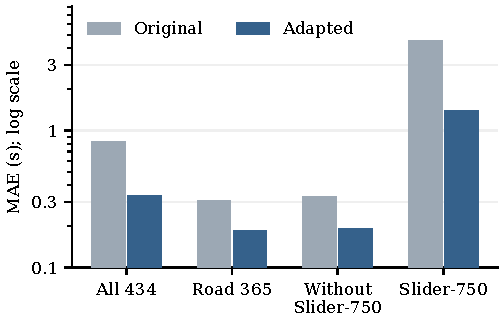
\includegraphics[width=.72\linewidth]{updates/figures/adaptation.pdf}
\caption{\textbf{Local effect of quality adaptation.} The corrected evaluator compares the original and adapted outputs on the same queries. A logarithmic vertical axis separates the road and Slider error scales. This figure reports exposed development evidence, with organizer-style negative-output interpolation applied to both variants. \evidence{N01}}
\label{fig:quality-adaptation}
\end{figure}

\paragraph{Comparison with organizer scores.}
\label{par:local-score-correspondence}
Our reconstruction matches the organizer-provided original relative error for nine of ten sequences after rounding. For Slider-750, we obtain 283.9\% rather than the organizer's 132\%; the adapted model scores 76.1\% under our local evaluator. The available records leave the source of this discrepancy unresolved. Reconciliation requires the organizer-aligned targets and exact evaluator version, so we report the adaptation gains under the local scoring contract. Appendix~\ref{app:competition-details} records the target correspondence and evaluation boundary.


\subsection{Matched attribution follow-up}
Section~\ref{sec:quality-adaptation} adds geometry-only, fallback, fixed-mixture, and router comparisons on identical query support. The earlier protocol above is retained to distinguish raw signed inference from organizer-style offline interpolation.
\FloatBarrier

\section{Additional sensor and benchmark illustrations}
\label{app:extra-diagnostics}
The following figures supply the sensor detail and score decompositions behind the compact main-text tables.
\subsection{Real sensor observations}

Figure~\ref{fig:real-evttc-scene} shows the appearance of the two sensor streams on an actual EvTTC road recording \citep{evttc}. The RGB frame records scene appearance, whereas the event view accumulates signed brightness changes during the preceding 100\,ms. Vehicle outlines, road markings, and background motion therefore appear differently in the two modalities. These are recorded observations rather than schematic renderings. The side-by-side views retain the coordinates of their respective cameras.

\begin{figure}[H]
  \centering
  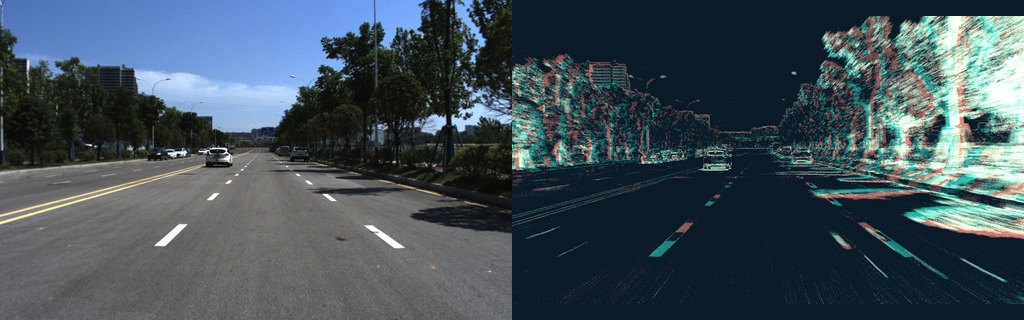
\includegraphics[width=\linewidth]{figures/evttc_ccrm_poster.jpg}
  \caption{\textbf{Real RGB and event observations from EvTTC.} Left: Blackfly left-camera frame 287 at $t=14.350374$\,s in recording \texttt{CCRm-low-0-overlap-0}. Right: Prophesee left-camera events in $[t-100\,\mathrm{ms},t)$, with positive counts in turquoise and negative counts in coral; overlap can appear pale. Counts use log scaling and an occupied-pixel 95th-percentile display scale. The RGB display swaps stored channels 0 and 2 to match the dataset publisher's visualization; the model-input crops preserve the runtime channel order. Images are resized for display and retain separate sensor coordinates. Source: EvTTC, Sun et al.\ \citep{evttc}; the same excerpt is used in the project website.}
  \label{fig:real-evttc-scene}
\end{figure}

The RGB view preserves scene appearance while event polarities reveal moving contours and contrast boundaries. The model receives localized object crops in a common coordinate frame across causal endpoints, preserving apparent scale change. Appendix~\ref{sec:real-inputs} shows the temporal crop triplets and twelve event input planes for this recording, with their timestamps and extraction provenance.


\subsection{Benchmark score decompositions}
\begin{figure}[htbp]
\centering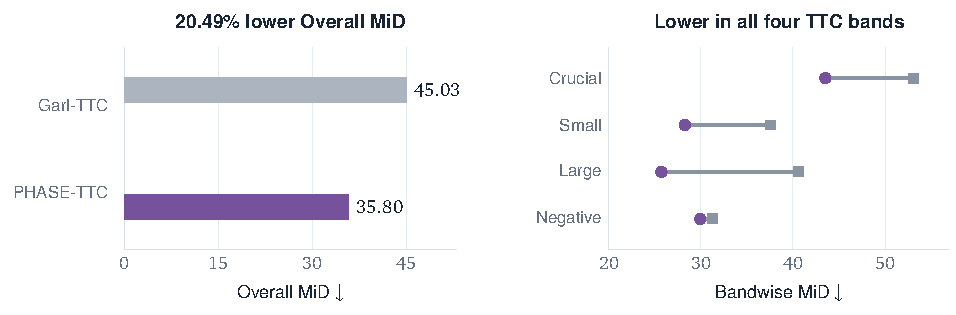
\includegraphics[width=\linewidth]{figures/rev_hero.pdf}
\caption{\textbf{Archived GarlTTC Test results, 28 October 2026.} Overall MiD and the four TTC bands compare the complete PHASE-TTC and Garl-TTC submissions. Both report 0\% scorer-defined failures across 6,762 tokens.}
\label{fig:official}
\end{figure}
\begin{figure}[H]
\centering
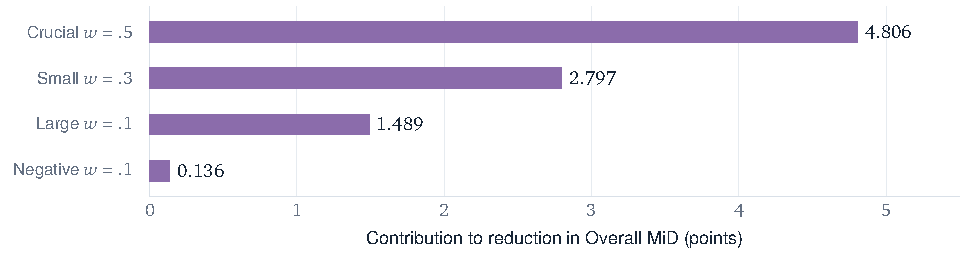
\includegraphics[width=.92\linewidth]{figures/rev_weighted.pdf}
\caption{\textbf{Bandwise contributions to the Overall MiD difference.} Crucial and small TTC account for about 82\% under the benchmark's $0.5/0.3/0.1/0.1$ weights. Table~\ref{tab:official-weighted-contributions} gives the rounding reconciliation. \evidence{B01,B02}}
\label{fig:official-weighted-contributions}
\end{figure}

\subsection{Transfer error distributions}
\begin{figure}[H]
\centering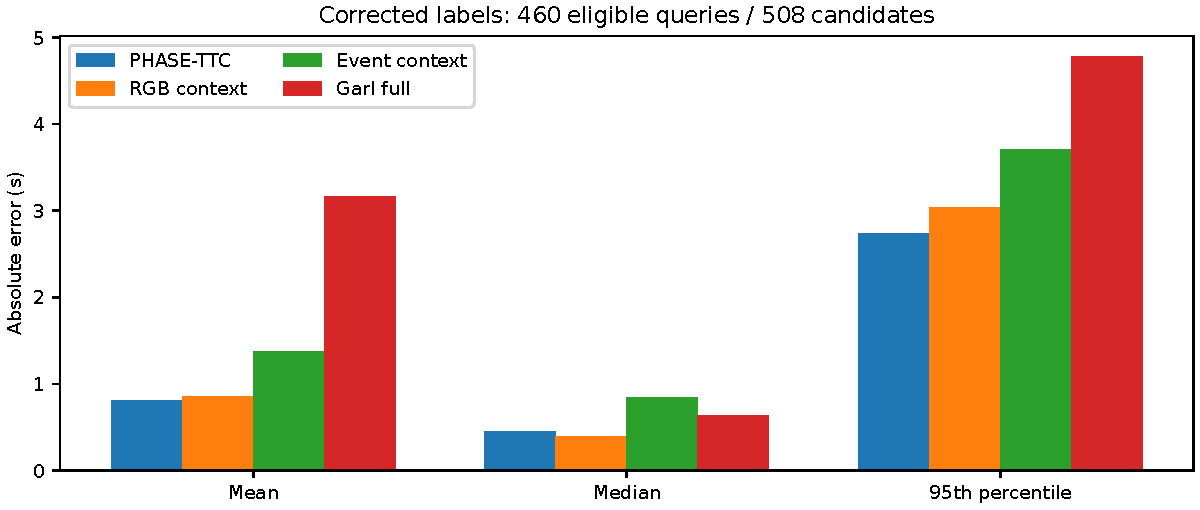
\includegraphics[width=.94\linewidth]{figures/audit_transfer_summary.pdf}
\caption{\textbf{Corrected frozen-transfer error summaries.} PHASE-TTC and RGB use the same \AuditTransferCount{} eligible queries after reassociating all 508 candidates. Lower point mean and p95 favor fusion; lower median favors RGB. Paired intervals are reported separately in Table~\ref{tab:audit-transfer-bootstrap}.}
\label{fig:transfer-tradeoff}
\end{figure}
\begin{figure}[htbp]
\centering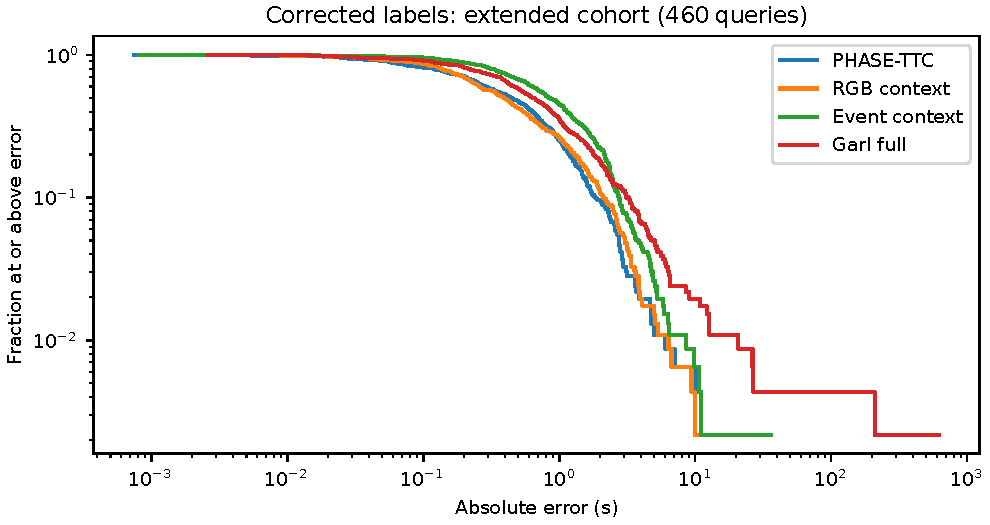
\includegraphics[width=\linewidth]{figures/audit_transfer_exceedance.pdf}
\caption{\textbf{Corrected absolute-error exceedance.} Curves include all \AuditTransferCount{} eligible transfer queries with equal query weights. No signed prediction is clipped and no extreme error is removed.}
\label{fig:transfer-exceedance}
\end{figure}

\section{The initial representation-learning programme}
\label{sec:early}

PHASE-TTC began as E-JEPA-TTC, a study of predictive event representations for time-to-contact estimation. The programme covered pooled and spatial embeddings, apparent expansion, and transport-conditioned residual dynamics. Some models improved TTC while losing the geometric behaviour that motivated them, so the experiments assessed accuracy, geometric consistency, and representation content separately.

The historical names distinguish otherwise similar version numbers. \emph{Causal Scale v5--v8} refers to synthetic operator tests, whereas \emph{Scientific Recovery V5--V8} refers to later real-data studies. The EvTTC and eAP A0/A1 experiments also used different data and metrics.

\begin{figure}[htbp]\centering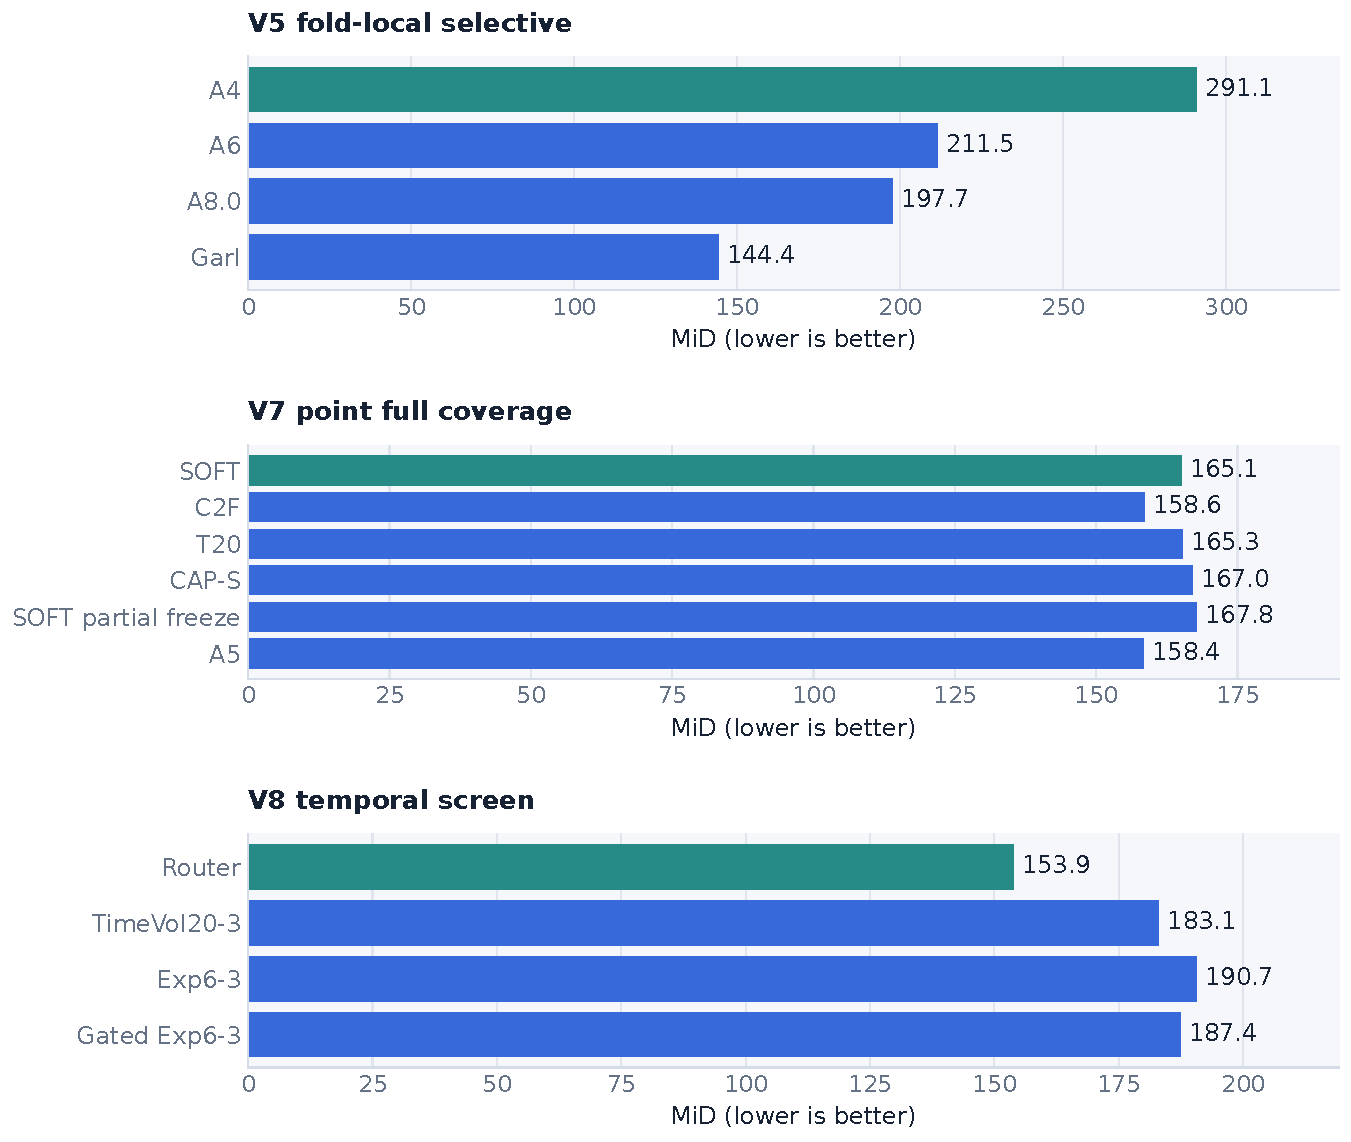
\includegraphics[width=\linewidth]{figures/early_ablation.pdf}
\caption{Early recovery results by experiment family; lower MiD is better.}\label{fig:early}
\end{figure}

\subsection{Global and dense representations on EvTTC}

The spatial-granularity comparison tests global pooling (A0) against a dense spatial readout (A1) under matched EvTTC conditions. Five sequence-grouped folds and seeds 7, 13, and 21 provide fifteen paired runs per model (Table~\ref{tab:early-evttc}).

\begin{table}[htbp]
\centering\small
\begin{tabular}{lrrr}
\toprule
Architecture & MAE (s) & Relative error (\%) & Selection score \\
\midrule
Global A0 & 1.0109 & 30.25 & 0.58452 \\
Dense A1 & 1.0067 & 30.55 & 0.59312 \\
\bottomrule
\end{tabular}

\caption{Global A0 and Dense A1 means over five EvTTC folds and three seeds.}
\label{tab:early-evttc}
\end{table}

The dense readout reduces mean absolute error while increasing relative error and the composite selection score. Its training cost is 1.58 times that of the compact globally pooled model under this protocol. Historical inference-timing observations remain in source E01 and are excluded from the persistent-service latency comparison.

Attention residuals, temporal KDA/Object-KDA, object-conditioned crops, and FlowMimic-style alignment all failed their selection criteria. Because those screens used different data or criteria, they do not extend the matched A0/A1 ranking. \evidence{E01}

\subsection{Representation variance and dynamic information}

The temporal-residual objective captured the desired dynamics under a slow synthetic nuisance process. Its mean dynamic $R^2$ was about $0.72$, versus $0.15$ for variance regularization. The latter maintained high embedding variance while preserving nuisance information, showing that variance alone was a poor proxy for useful temporal content.

Changing the nuisance on every frame reversed the result: the residual objective's dynamic $R^2$ became negative, while the variance control reached about $0.74$. Later probes kept both level and change features and varied the nuisance process. Neither effective rank nor per-dimension standard deviation demonstrated TTC-relevant content on its own. \evidence{E02,E12}

\subsection{Object identity and crop geometry}

Object-level eAP/GarlTTC requires an explicit query because several annotated objects can share one event frame while having different TTC values. Object-LHR resolved the ambiguity by cropping the selected object at both endpoints before estimating temporal scale.

Independent resizing erased much of the apparent scale change required by the geometric head. Object-Expansion v2 stabilized the output by predicting sign and log inverse-TTC magnitude; Object-Signed-Expansion v3 combined them in one expansion coordinate and added ordered temporal features plus box motion. Perturbation tests showed strong dependence on box motion and little response to events, so this accuracy could not be credited to event representation learning.

Object Event v4 placed three causal endpoints in one common crop, preserving apparent growth and separating the neural event path from the motion ablation. The object query and its coordinate system became part of the model specification. Earlier variants used different conditions and remain separate experiments.

\subsection{Physical tests of the scale operator}

The frozen v4.31 matcher passed representation-stability checks but failed the zoom, reversal, and translation requirements. Incomplete source provenance and missing validation records also prevented its selection. Its foreground, height, pseudoflow, and correspondence diagnostics motivated a new scale estimator.

For two apparent heights $h_{t-1}$ and $h_t$ separated by $\Delta t$, the Causal Scale operator defines
\begin{equation}
 r_t=\log h_t-\log h_{t-1},\qquad
 \widehat{\tau_t^{-1}}=\frac{\exp(r_t)-1}{\Delta t}.
 \label{eq:early-scale}
\end{equation}
Under idealised constant-speed approach, this gives inverse TTC at the newer endpoint. Changes in shape, viewpoint, occlusion, or relative motion can violate the geometric assumptions. For $\hat\tau_t=\Delta t/(\exp(r_t)-1)$, the sensitivity is
\begin{equation}
 \frac{\partial\hat\tau_t}{\partial r_t}
 =-\frac{\Delta t\exp(r_t)}{(\exp(r_t)-1)^2}.
\end{equation}
The derivative grows without bound as $r_t$ approaches zero. Output clipping can contain the resulting TTC value, but it cannot improve the scale measurement.

The learned foreground failed to reproduce the ideal operator on held-out synthetic data. Causal Scale v5 reached correlation $0.92$ with translation leakage $0.027$, missing both requirements. V7 reduced leakage to $0.0034$ and symmetric TTC error to $0.25$, but correlation stayed at $0.92$ and the validation result did not transfer to the new synthetic group.

Causal Scale v8 selected on both mean and worst-group performance across independent synthetic groups. Fixed symmetric smoothing supported sparse endpoints, and a final CVaR loss emphasized large ratio errors. Correlation remained below the required threshold in every group. A subsequent real-data screen evaluated the operator under exploratory conditions. \evidence{E13,E14,E15}

\subsection{Foreground supervision in the first eAP screens}

The first eAP screens used a common object crop, three event endpoints, and oracle boxes; they did not evaluate detection. A0 learned a weak rectangular foreground target. A1 replaced it with height, width, and centre supervision. A1-FR added a full-resolution decoder, A1-DF used deeper features, and A1-DF-R supervised the pair ratio directly. A3 kept the A1 architecture and trained with RGB-derived SAM masks. All screens reused public validation data.

\begin{table}[htbp]
\centering\small
\begin{tabular}{lrr}
\toprule
Arm & MiD $\downarrow$ & Failure (\%) \\
\midrule
A1 geometry & 346.829 & 9.961 \\
A3 SAM distilled & 353.635 & 10.889 \\
Garl trained matched & 203.634 & 0.000 \\
\bottomrule
\end{tabular}

\caption{Selected early eAP public-validation results for A1, A3, and matched Garl. A0 and the A1 architecture variants described in the text are not tabulated here.}
\label{tab:early-screen}
\end{table}

A3 did not improve on A1, and both scored worse in aggregate MiD than matched Garl. The diagnostics showed that estimating absolute height did not guarantee recovery of its temporal derivative. Garl achieved lower aggregate error but predicted positive TTC for receding cases, leaving signed motion unresolved.

A4 distilled local spatial relations from a frozen DINOv3 RGB teacher into an event student; A4D also learned changes in those relations across endpoints. Both used RGB during training and events at inference. \evidence{E25,E26}

The A4 scaling follow-up (A4-S1) retained the 355,118-parameter student and the same 2,048 public-validation samples. Training increased from 2,048 to 8,192 samples, while the DINO distillation weight increased from $\lambda=4$ to $8$, selected by three-fold sequence cross-validation within training. With seed 7, eighteen training epochs, and checkpoint selection at epoch 15, sequence-macro MiD fell from 322.7 to 262.8, failures from 11.08\% to 8.59\%, and log-scale-ratio correlation rose from 0.260 to 0.448. Matched Garl remained lower at 203.6 MiD with no failures. The 18.5\% MiD reduction combines more training data with a changed loss weight; the preregistered 8,192-sample $\lambda=4$ control remained unexecuted at that closure. Attribution to either change alone and replication across seeds therefore remained unresolved. A5 and A6 subsequently varied TTC specialization and transport while monitoring the inherited geometry. \evidence{H_A4_S1}

\subsection{Fold-specific producer training}

The first grouped-development run inherited an A4 parent trained on all nine development sequences, including each held-out outer group. That comparison was excluded from selection, and the relationally distilled producer (A4) was retrained inside every outer fold. The corrected study initialized A6 and A8.0 from the matching fold-local parent and trained Garl from scratch.

The comparison matched samples, targets, training budget, metric, and oracle-ROI access. The E-JEPA-family branch used three endpoints and twelve channels; Garl used two endpoints and forty channels. Checkpoint selection still used the outer-development split, and TTC buckets shaped the initial 8,192-token sample. Thus, the correction removed parent exposure without turning the study into a blind test or a target-free sample. \evidence{E03}

\begin{table}[htbp]
\centering\small
\begin{tabular}{lrrr}
\toprule
Model & Parameters & MiD $\downarrow$ & Failure (\%) \\
\midrule
A4 parent & 355,118 & 291.088 & 9.448 \\
A6 transport & 498,130 & 211.509 & 7.849 \\
A8.0 dual transport & 627,827 & 197.691 & 7.019 \\
V6.1 radius 2 & 627,827 & 194.122 & 6.689 \\
A5 causal & 424,274 & 155.472 & 4.761 \\
Garl local matched & 24,674,178 & 144.353 & 0.000 \\
\bottomrule
\end{tabular}

\caption{Scientific Recovery V5--V6 results on 8,192 tokens from nine sequences, three folds, and seed 7.}
\label{tab:early-v5v6}
\end{table}

A8.0, which freed transport while retaining the frozen parent geometry, improved MiD over A6 by 13.8 points; the paired 95\% interval was $[-17.7,-10.1]$. It still exceeded the preregistered MiD threshold of 175 and remained behind Garl, so V5 produced no candidate.

Sequence-scoped track identifiers and preserved token/target IDs made the fold-local correction auditable through the full training lineage. \evidence{E03,E05}

\subsection{Transport capacity and geometric retention}

Increasing the transport radius from one to two did not yield a clear V6 gain: V6.1 reduced mean MiD relative to A8.0, but the paired interval $[-8.2,1.0]$ crossed zero. A5 achieved lower TTC error than the geometry-frozen variants while weakening their geometric dynamics, which kept accuracy and mechanism retention as separate criteria.

V7 tested soft geometric distillation, coarse-to-fine transport, extra temporal bins, greater capacity, and partial freezing. Under full-coverage point evaluation, A5 scored 158.4 MiD and served as the reference. Promotion required both lower TTC error and retained geometric behaviour. \evidence{E04,E06,E07,E08,E09,E10,E11}

\begin{table}[htbp]
\centering\small
\begin{tabular}{lrrr}
\toprule
Arm & Point MiD & Delta vs A5 & Paired 95\% interval \\
\midrule
A5 reference & 158.449 & -- & -- \\
SOFT & 165.116 & +6.668 & [+3.084, +10.547] \\
C2F & 158.573 & +0.125 & [-3.025, +3.432] \\
T20 & 165.260 & +6.812 & [+2.290, +11.514] \\
CAP-S & 167.025 & +8.576 & [+3.735, +13.630] \\
SOFT partial freeze & 167.826 & +9.378 & [+5.359, +13.272] \\
\bottomrule
\end{tabular}

\caption{V7 full-coverage MiD relative to A5, using seed 7 and three outer folds.}
\label{tab:early-v7}
\end{table}

Every V7 arm failed at least one mechanism, geometry, or confirmation requirement, and none advanced to confirmation seeds. More temporal bins, capacity, and partial freezing did not close the comparator gap. The JEPA objective was inactive in these runs, so their results provide no evidence about JEPA pretraining.

A post-hoc A5/C2F analysis found complementary errors. Separating a deployable feature-based router from a target-aware oracle motivated the subsequent prospective nested-routing comparison. \evidence{E07,E08,E09,E10,E11}

\subsection{Nested routing and predictive-learning attribution}

Only the nested A5/C2F router passed V8's candidate screen; all three temporal-representation interventions failed it. \evidence{E16,E17,E18,E19}

\begin{table}[htbp]
\centering\small
\begin{tabular}{lrrr}
\toprule
Arm & MiD & Finite (\%) & Stored gate \\
\midrule
router & 153.877 & 100.00 & True \\
timevol20\_3 & 183.092 & 95.25 & False \\
exp6\_3 & 190.711 & 94.10 & False \\
gated\_exp6\_3 & 187.400 & 94.80 & False \\
\bottomrule
\end{tabular}

\caption{V8 seed-7 MiD and finite coverage for the router and temporal-representation arms.}
\label{tab:early-v8}
\end{table}

The seed-7 router improved on A5 by 4.6 MiD points. Its scores were 153.9, 153.3, and 156.0 for seeds 7, 13, and 23. All three runs reused the same development sequences and estimate optimization stability, not independent external replication. Matched Garl seed replications were unavailable.

The stored V8 summaries support point estimates, finite coverage, and selection outcomes. They do not specify enough aggregation detail to reconstruct valid uncertainty intervals, so none are reported.

A post-training path replay located the trained model's dependence. The analytic height path had high error, and adding a residual without transport changed little. Transport plus the residual produced the main improvement; history added a smaller gain. Because the replay disabled paths without retraining, it measures use inside this trained graph rather than the effect of retraining each ablation. \evidence{E16,E20,E21}

\begin{table}[htbp]
\centering\small
\begin{tabular}{lr}
\toprule
Replay intervention & MiD $\downarrow$ \\
\midrule
analytic only & 373.176 \\
analytic residual & 373.596 \\
analytic residual transport & 163.231 \\
analytic residual transport history & 155.824 \\
analytic transport & 373.176 \\
\bottomrule
\end{tabular}

\caption{V8 post-training path replay showing MiD for the analytic, residual, transport, and history paths.}
\label{tab:early-factorial}
\end{table}

The H2 diagnosis was shortcut/residual dominance: the analytic height path did not explain the trained model's advantage. This motivated a measurement interface with less dependence on explicit height estimation. The diagnosis did not rule out useful geometry or transport features.

V8 tested JEPA attribution through D0--D4. The meta-router had no single transferable encoder, so A5 supplied the downstream reference. D2 froze the JEPA encoder, D3 fine-tuned part of it, and scratch, random-frozen, and shuffled-future arms controlled for downstream capacity and temporal correspondence. \evidence{E22,E24}

\begin{table}[htbp]
\centering\small
\begin{tabular}{lrrrrr}
\toprule
Arm & 1\% & 5\% & 10\% & 25\% & 100\% \\
\midrule
Scratch (D0) & 265.20 & 286.35 & 277.40 & 270.97 & 276.35 \\
Random frozen (D1) & 379.82 & 369.40 & 361.68 & 370.87 & 365.44 \\
JEPA frozen (D2) & 380.09 & 380.01 & 380.04 & 379.97 & 380.12 \\
JEPA partial fine-tuning (D3) & 379.51 & 379.40 & 379.41 & 379.26 & 379.62 \\
Shuffled future (D4) & 379.02 & 379.01 & 378.89 & 378.89 & 379.12 \\
\bottomrule
\end{tabular}

\caption{V8 seed-7 controls on the same three-fold OOF queries, recomputed from the recovered signed prediction artifacts with one sequence-macro evaluator. All five arms and nominal label fractions appear together. Historical aggregate values for D2/D3 are retained in the source data; their small discrepancy from this recomputation is documented below.}
\label{tab:early-jepa}
\end{table}

D2 and D3 produced finite predictions with no recorded failures, but neither passed the causal-benefit criterion against scratch, random-frozen, and shuffled-future controls. V8 provided no positive JEPA attribution, and the next experiments focused on the measurement interface and feature usefulness. \evidence{E23}

The recovered aggregate matches the archived E23 file hash, but rescoring its associated predictions differs by up to 0.177 MiD for D2/D3. Table~\ref{tab:early-jepa} therefore uses the recomputed predictions for all arms rather than mixing cached aggregates with newly calculated controls. Scratch remains substantially better than either JEPA arm at every fraction, by 94 to 115 MiD. The frozen JEPA encoder is also worse than the frozen random encoder at every fraction, by 0.3 to 18.4 MiD. The D2, D3, and D4 scores each change by less than 0.4 MiD between 1\% and 100\% of the labels, which is the pattern expected from nearly constant outputs; we did not diagnose that degeneracy further, so the study shows that these arms failed, not why. The origin of the small cached-aggregate discrepancy is unresolved; it does not alter that ordering. Only seed 7 completed this attribution study.

Two further negative results from the project records are not part of the hash-verified evidence and are reported here for completeness. In an earlier dense level--dynamics screen, four label-free pretraining arms and a scratch control all produced nearly constant downstream predictions, with validation MiD between 201.83 and 202.01 and a prediction-to-target standard-deviation ratio of order $10^{-6}$ to $10^{-3}$; because scratch failed in the same way, that screen is uninformative about JEPA. A self-supervised and supervised experiment on synthetic CARLA sequences worsened transfer; its data were withdrawn and only compact negative metrics were kept.

\section{Temporal information and phase refinement}
\label{sec:temporal-recovery}

The temporal studies (V9--V12 in the historical records) ask whether causal motion information improves phase estimates beyond the existing expert outputs. The controls removed transport fields, disrupted correspondence or order, reduced the expert set, and replaced recurrence with unordered aggregation. Prespecified comparisons used sequence-level uncertainty and kept separately trained producer families distinct.

\subsection{E-Clock: incremental information in transport features}

E-Clock represented signed TTC in benchmark phase. With $\Delta=0.1$ seconds,
\begin{equation}
 \phi(T)=-\log(1-\Delta/T),\qquad
 d(\hat T,T)=10^4\lvert\phi(\hat T)-\phi(T)\rvert.
\end{equation}
The phase exists only on the admissible signed-TTC domain, and $d$ measures phase error rather than seconds. Historical A5 replay, raw inverse-TTC evaluation, and bounded deployment output follow different numerical conventions and are reported under their original definitions.

Transport helped X0's direct-phase model, but did not close the gap to A5. With architecture, capacity, matcher, and input structure fixed, DYN-U scored 225.0 MiD versus 270.6 for the zeroed BASE-U control. Canonical A5 and PAIR-U scored 158.4 and 158.1. X0.5 next conditioned the transport fields on A5.

X0.5 found no confirmed incremental value from nine frozen transport fields. DYN9 scored 155.2 MiD, against 158.7 for calibrated A5 and 175.0 for a target-blind within-sequence shuffle. The difference from calibration was $-3.5$ with hierarchical 95\% interval $[-11.4,3.5]$; the interval against raw A5 also crossed zero. Leave-one-sequence-out tuning kept normalization and ridge fitting outside the outer meta-test. DYN9 did not meet the incremental-utility criteria, so the conditional X1 adapter was not trained. \evidence{M_X0,M_X05,M_X05_GATE}

\subsection{Pair routing and local motion fields}

% Generated by research/middle_tables.py; do not edit numeric values.
\begin{table}[tbp]
\centering\small
\caption{Pair routing (Stage 61) and local-field experiments (Stage 62).}
\label{tab:middle-mechanisms}
\setlength{\tabcolsep}{5pt}
\begin{tabular}{l@{\hspace{18pt}}r@{\hspace{18pt}}r@{\hspace{18pt}}r}
\toprule
Arm & MiD & Queries & Finite \\
\midrule
\multicolumn{4}{l}{\textbf{Stage 61}} \\
R1 & 152.855 & 8,192 & 100\% \\
R2 & 150.876 & 8,192 & 100\% \\
R2\_SHUFFLE & 185.429 & 8,192 & 100\% \\
RouterR & 153.877 & 8,192 & 100\% \\
\midrule
\multicolumn{4}{l}{\textbf{Stage 62}} \\
RouterR & 153.877 & 8,192 & 100\% \\
X2\_A5\_REPLAY & 162.205 & 8,192 & 100\% \\
X2\_GLOBALPOOL & 155.351 & 8,192 & 100\% \\
X2\_LOCALFIELD & 155.463 & 8,192 & 100\% \\
X2\_SHUFFLEFIELD & 155.827 & 8,192 & 100\% \\
X2\_TIMESWAP & 155.585 & 8,192 & 100\% \\
\bottomrule
\end{tabular}
\par\vspace{4pt}
\begin{minipage}{0.98\linewidth}\footnotesize Sequence-macro MiD, evaluated on nine sequences and three folds per stage. Lower is better. \evidence{M_STAGE61,M_STAGE62}\end{minipage}
\end{table}


R2 gave Stage61's lowest point estimate but did not meet the incremental-utility criterion. Across 8,192 queries from nine sequences, MiD was 150.9 for R2, 152.9 for R1, 153.9 for RouterR, and 185.4 for shuffled R2. The paired hierarchical intervals comparing R2 with R1 and RouterR crossed zero.

Stage62 could not isolate a local-field benefit. LOCALFIELD scored 155.5 MiD, close to GLOBALPOOL at 155.4, SHUFFLEFIELD at 155.8, and TIMESWAP at 155.6. Although all improved on this producer family's 162.2 A5 replay, LOCALFIELD did not meet the mechanism criteria against its controls.

The canonical V7 A5 and the A5 retrained inside the nested router use different checkpoints and training exclusions. Their scores remain separate despite overlap in architecture and queries. \evidence{M_STAGE61,M_STAGE62}

\subsection{Temporal features, regret estimation, and geometry support}

Stage63 repaired the experimental base by standardizing temporal bins and restoring one FP32 producer state. Equivalent fixed-grid pooling also made CUDA backward deterministic on the prescribed shapes.

The raw-time study compares a temporal event-rate residual (RAW-L1) with total-count redistribution across bins (COUNT-L1), a bin-permutation control, and a state-only residual with event-rate inputs zeroed (STATE-L1). Their MiD scores are 162.2, 157.2, 164.3, and 150.7, respectively. The better count and state controls leave the proposed temporal-rate benefit unsupported. A later regret-based expert router (RISK17) reaches 146.0 MiD, but omitted validation controls and their execution order prevent acceptance of that result.

Convex expert routing (SIMPLEX17) improves the point estimate by 2.0 MiD over the frozen regret router, reaching 144.0. Hierarchical and sequence-only 95\% difference intervals, $[-5.5,1.2]$ and $[-4.7,0.3]$, both include zero. The reduced-gating, unconstrained, and PAIR-permuted alternatives score 143.9, 144.5, and 149.2. Across these four arms, twelve fits and 18,000 CPU float64 updates over three folds preserve the registered comparison; the small routing gain remains statistically unresolved.

Stage68 stopped before fitting because the normal-flow estimator supplied too little valid geometry. Only 368 of 8,192 tokens had any valid window; 583 of 16,384 windows supported the full-affine fit, and none supported the reduced-isotropic fit. Fold support rates of 4.9\%, 5.6\%, and 3.0\% all missed the fixed 20\% threshold. Insufficient support excluded the subsequent ridge and neural fits. The support limitation concerns this normal-flow estimator under the tested conditions. \evidence{M_STAGE63_REPAIR,M_STAGE64,M_STAGE65,M_STAGE69_DECISION,M_STAGE67_DIAGNOSTICS,M_STAGE67_DECISION,M_GEOMETRY}

\subsection{SIMPLEX-T: residual phase refinement}

Expert selection constrains the output to the available expert phases. SIMPLEX-T instead anchors a residual predictor at their label-free median,
\begin{equation}
 \hat\phi_t=\Pi\!\left(\operatorname{median}_{k}\phi_{t,k}
                  +0.03\,g(h_t)\right),
\end{equation}
where $h_t$ summarizes masked history and $\Pi$ enforces the numerical output bounds. Unlike expert selection, this residual can leave the experts' convex hull. A separate cost head estimates relative losses of the original experts; it does not estimate the corrected prediction's risk. Both the recurrent and bounded-window Transformer versions mask missing history and start with zero-initialized output heads.

The primary recurrent model uses two 160-unit GRU cells. It maps expert and timing features to phase, auxiliary phase quantiles, and relative expert costs. The quantiles are not calibrated collision probabilities. History is retrospective within the current query ROI; the experiments did not verify persistent object tracking.

The original residual-context campaign (T6) completed 72 fits and 180,000 saved optimizer updates on OLD\_DEV: 8,192 queries from nine sequences in three folds. H1 uses the current observation; H8 adds up to seven past slots. Each head shares the frozen expert producers. Across head seeds 7, 13, and 23, H8 reached mean MiD 121.8 versus 133.1 for H1. The mean paired-loss difference was $-11.3$, with hierarchical 95\% interval $[-16.2,-6.6]$ conditioned on these heads and reused development sequences. This estimates a context benefit within that lineage, rather than independent external replication. \evidence{H_T6}

\begin{table}[htbp]
\centering\small
\begin{tabular}{p{0.30\linewidth}rp{0.43\linewidth}}
\toprule
Original T6 head, seed 7 & MiD $\downarrow$ & Training condition \\
\midrule
Current observation (H1) & 132.832 & One observation, 160-unit recurrent cells \\
Past context (H8) & 121.646 & Eight chronological slots, same cell width \\
Reversed past & 121.225 & Trained with reversed past order \\
Repeated current & 131.211 & Current observation repeated across eight slots \\
Expert selector & 143.504 & Selection in place of residual correction \\
Latent, current only & 171.057 & Added hidden producer coordinates, H1 \\
Latent, past context & 184.072 & Added hidden producer coordinates, H8 \\
Zeroed latent, H8 & 120.910 & Same latent-input architecture with coordinates zeroed \\
\bottomrule
\end{tabular}
\caption{Trained residual-context controls from the original 72-fit T6 campaign on OLD\_DEV (8,192 queries, nine sequences, three folds). These rows report separately trained controls, not post-training interventions on one fixed model. Historical identifiers are H1/H8-C160, PAST\_REVERSED, REPEAT\_CURRENT, SELECTOR, LATENT, and LATENT\_ZERO. \evidence{H_T6}}
\label{tab:original-t6}
\end{table}


The trained controls refine that interpretation. Repeating the current observation through eight slots failed to match past context, while expert selection remained worse than residual correction. Training with reversed past order matched chronological H8 within the recorded uncertainty; this model could learn the reversed convention, so the result does not establish dependence on chronological order in a fixed trained model. Adding hidden producer coordinates degraded both H1 and H8, whereas removing those coordinates recovered the scalar-feature result. This negative finding concerns the tested latent interface and does not identify misalignment as its sole cause or exclude other useful latent representations. \evidence{H_T6}

A subsequent extension completed 24 fits and 60,000 saved updates. It tested H16, reduced expert sets, and set aggregation while reusing the original H8 endpoints and retaining H8 as the registered candidate. These are separate campaign totals; reused endpoints are not new fits. Seeds 7, 13, and 23 retrained only the heads over shared expert producers.

H16 reduced MiD in every head seed. Across all three, mean paired loss was 119.2 for H16 and 121.8 for H8, a difference of $-2.5$ with hierarchical 95\% interval $[-5.2,-0.1]$. Seed 7 had already informed exploration. Seeds 13 and 23 alone gave $-2.4$ with interval $[-5.2,0.04]$, which crosses zero. The analysis averages losses across shared-producer heads, rather than ensemble predictions or full-system replications. \evidence{M_TEMPORAL_MODEL,M_PHASE_CONTRACT,M_SIMPLEX}

% Generated by research/middle_tables.py; do not edit numeric values.
\begin{table}[tbp]
\centering\small
\caption{H16 and H8 temporal heads on OLD\_DEV.}
\label{tab:middle-replication}
\setlength{\tabcolsep}{5pt}
\begin{tabular}{lrrrr}
\toprule
Head seed(s) & H8 MiD & H16 MiD & $\Delta$ MiD & Hierarchical 95\% CI \\
\midrule
7 (observed) & 121.646 & 118.866 & -2.781 & [-5.879, +0.301] \\
13 & 121.841 & 119.697 & -2.144 & [-5.317, +0.712] \\
23 & 121.865 & 119.162 & -2.703 & [-5.514, -0.071] \\
\midrule
New seeds 13/23 & 121.853 & 119.429 & -2.424 & [-5.244, +0.041] \\
All three seeds & 121.784 & 119.241 & -2.543 & [-5.213, -0.111] \\
\bottomrule
\end{tabular}
\par\vspace{4pt}
\begin{minipage}{0.98\linewidth}\footnotesize Nine sequences, 8,192 queries, and three folds. Delta is H16 minus H8; multi-seed rows average paired losses. Seed 7 had been evaluated previously. All heads share fixed expert producers. \evidence{M_SIMPLEX}\end{minipage}
\end{table}


\begin{figure}[tbp]
\centering
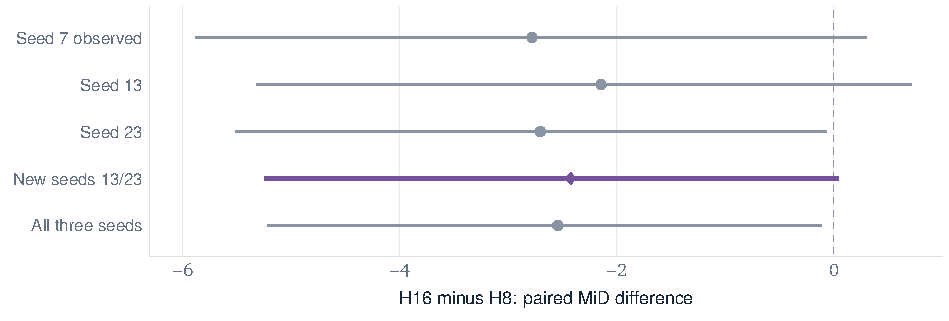
\includegraphics[width=0.98\linewidth]{figures/rev_h16.pdf}
\caption{Paired H16-minus-H8 MiD differences for three head seeds on the historical development set (OLD\_DEV).}
\label{fig:middle-h16}
\end{figure}

The full expert/context model outperformed every registered reduction. FULL-C0 scored 121.4 MiD, versus 127.8 for A5-only, 126.7 for C2F-only, and 124.7 for A5 plus PAIR. Unordered aggregation with age reached 122.4; removing explicit time gave 123.7. Each reduction failed the accuracy screen or its small-excess-error bound. The experts themselves can encode temporal information, so this comparison does not isolate recurrence as the source of the gain.

The analytic EWMA/transport control lost to H8 on every sequence, scoring 155.4 versus 121.6 MiD; the hierarchical interval for the 33.8-point difference was $[17.1,51.0]$. WIDE averaged 119.0 across three head seeds, but its intervals against both H8 and H16 crossed zero. It was not promoted. \evidence{M_SIMPLEX,M_EWMA,M_WIDE}

\subsection{Capacity and teacher-feature coverage}

Stage70--76 and the V11 capacity extension planned direct, pairwise-predictive, trajectory, and temporal-permutation comparisons at approximately 2M, 4M, and 8M parameters. The 4M trajectory model was primary. The proposed 30,000-query set covered 27 sequences; extra timestamps increased density, not the number of independent acquisitions.

The V11 audit found teacher features for 4,775 historical tokens and none for the other 25,225. Matching token IDs also left ROI construction, RGB preprocessing, and teacher provenance unresolved.

Stage70 ended with both completed and unfinished endpoints. The partial record supplies no capacity ranking and no evidence that unlabeled JEPA pretraining improved SIMPLEX-T. \evidence{M_CAPACITY_PROTOCOL,M_CAPACITY_AUDIT,M_STAGE70_LEDGER}

\section{Transfer, output stability, and runtime}
\label{sec:transfer-context}

\subsection{Development, training, and transfer populations}

The historical development set (OLD\_DEV) informed model selection, while the forty-sequence fitting set (TRAIN40) includes training examples. Transfer experiments evaluate frozen models under separate dataset-specific input construction. EvTTC and Forward Collision Warning Data (FCWD) instead evaluate frozen models with dataset-specific adapters. FCWD contains three driving sequences with paired events, frames, and LiDAR-derived TTC \citep{eventaided}. The expanded EvTTC set adds timestamps to the same 32 sequences rather than a new holdout.

The earlier H8/TRAIN40 route predates the final refit in Section~\ref{sec:train40}. A5 and C2F each received 49,932 updates, the pair head 6,840, and each of three H8 heads 2,500. Its 88,744 training predictions diagnose fit but cannot estimate unseen-scene performance. Inference used events, while training also used an RGB teacher and geometric supervision.

The initial EvTTC evaluation had 946 valid targets among 1,024 queries from 32 sequences; the expansion had 3,640 among 3,947. FCWD contributed 597 eligible targets among 630 queries from three previously exposed sequences. Rows without ground truth remain unscored; all reported methods return finite predictions on the eligible rows. Full RGB/event Garl was omitted from FCWD because the RGB-to-event mapping had not been verified. \evidence{M_SCIENCE_AUDIT,M_V12_EVTTC_946,M_V12_EVTTC_3640,M_V12_FCWD_597}

\subsection{Input and output conditions}

H8 used retrospective event history and supplied oracle ROI metadata. Garl event-only used its native pair of event windows, while Garl full added RGB. The systems differed in context and input construction. EvTTC projected RGB to events with calibrated rotation but no depth-dependent parallax correction. These transfer adapters do not reproduce the published benchmark protocol.

RGB synchronization was corrected before full Garl evaluation. Selected images had to lie within 1\,ms of each event endpoint and about 100\,ms apart; the largest admitted offset was 453\,$\mu$s. The runner strictly loaded the released checkpoint and upstream normalization. The RGB extension followed inspection of event-only results, making this a development comparison with frozen weights.

H8 bounds TTC at $\pm60$ seconds. Garl keeps its native scale-ratio division, which emits very large finite values when the estimated scales nearly match. Full-population metrics retain those native predictions. \evidence{M_TRANSFER_REPORT}

\subsection{Transfer results and metric-dependent rankings}

% Generated by research/middle_tables.py; do not edit numeric values.
\begin{table}[tbp]
\centering\small
\caption{Frozen H8 and Garl models evaluated on EvTTC and FCWD.}
\label{tab:middle-transfer}
\setlength{\tabcolsep}{5pt}
\begin{tabular}{lrrrr}
\toprule
Method & MAE (s) & Median AE (s) & RMSE (s) & RTE (\%) \\
\midrule
\multicolumn{5}{l}{\textbf{EvTTC: 946 eligible / 1,024 queries; 32 sequences}} \\
H8 / head 7 & 1.321 & 0.766 & 3.027 & 62.35 \\
H8 / head 13 & 1.353 & 0.731 & 3.206 & 62.92 \\
H8 / head 23 & 1.409 & 0.738 & 3.392 & 68.87 \\
Garl event & 8.048 & 0.997 & 159.247 & 293.47 \\
Garl RGB + event & 1.868 & 0.692 & 7.875 & 76.77 \\
\midrule
\multicolumn{5}{l}{\textbf{EvTTC expanded: 3,640 / 3,947; same 32 sequences}} \\
H8 / head 7 & 1.361 & 0.722 & 3.475 & 53.70 \\
H8 / head 13 & 1.395 & 0.699 & 3.618 & 54.52 \\
H8 / head 23 & 1.456 & 0.702 & 4.003 & 59.15 \\
Garl event & 4.560 & 0.958 & 83.896 & 161.12 \\
Garl RGB + event & 94.510 & 0.661 & 5561.622 & 5180.18 \\
\midrule
\multicolumn{5}{l}{\textbf{FCWD: 597 / 630; three sequences}} \\
H8 / head 7 & 1.778 & 0.675 & 3.588 & 30.20 \\
H8 / head 13 & 1.597 & 0.580 & 3.258 & 27.41 \\
H8 / head 23 & 1.569 & 0.598 & 3.109 & 27.48 \\
Garl event & 2.146 & 0.602 & 5.072 & 26.89 \\
\bottomrule
\end{tabular}
\par\vspace{4pt}
\begin{minipage}{0.98\linewidth}\footnotesize Scores use queries with valid TTC targets; prediction coverage is 100\% on these queries. H8 bounds TTC at $\pm60$\,s, while Garl retains its native signed outputs. The FCWD comparison uses event-only inputs. \evidence{M_V12_EVTTC_946,M_V12_EVTTC_3640,M_V12_FCWD_597}\end{minipage}
\end{table}


The two EvTTC blocks of Table~\ref{tab:middle-transfer} were computed before the target-association audit and use the superseded CCRs-1 low/medium label assignment (Appendix~\ref{app:target-association}). The source ledgers carry the label hashes of that assignment; it affects 64 of the 1,024 candidate queries in the first block and 253 of 3,947 in the second, in two of the 32 sequences. These H8 and Garl values have not been recomputed with corrected targets and are retained as historical record only. The FCWD block is unaffected.

H8 had the lowest mean error on the first 946 EvTTC targets: its three heads reached 1.32--1.41 seconds MAE, versus 8.05 for Garl event-only and 1.87 for Garl full. Garl full had the best median, 0.69 seconds versus 0.73--0.77 for H8.

The 3,640-target expansion showed the same split. H8 achieved 1.36--1.46 seconds MAE, Garl event-only 4.56, and Garl full 94.51. Yet Garl full retained the best median at 0.66 seconds, ahead of H8's 0.70--0.72. Rare near-singular scale ratios drove Garl full's mean, so native-output and matched-clipping results remain separate.

On FCWD, H8 led in MAE at 1.57--1.78 seconds versus 2.15 for Garl event-only. Garl led in mean relative TTC error at 26.9\%, compared with 27.4--30.2\% for H8. These rankings weight the TTC distribution differently, and only three sequences were available for clustered uncertainty. \evidence{M_V12_EVTTC_946,M_V12_EVTTC_3640,M_V12_FCWD_597}

\subsection{Historical execution-study boundary}

Earlier profiling separated prepared-input heads from a shared-GPU query adapter. The adapter included repeated ROI/voxel reading and preparation, motivating bounded caching and transfer scheduling in the efficient-context study. These measurements do not describe the final persistent service. Their complete timing tables remain archived in \path{tables/middle_cost.tex} and sources M\_HEAD\_COST and M\_ROUTE\_COST, rather than entering this article's deployment-latency comparison. Sections~\ref{sec:runtime} and~\ref{sec:local-hardware} report persistent execution.

CUDA graphs reduced recorded A5 launches from 5,877 to 1,270 while preserving the tested outputs, losses, RNG state, and gradients. A later window measured 41.78 versus 32.89 updates/min, but host load and data wait also changed, so the run did not isolate graph speedup. Adaptive caching reached 26.31 updates/min against a 36.75 reference and failed its throughput test. \evidence{M_HEAD_COST,M_ROUTE_COST,M_ROUTE_REPORT,M_ENGINEERING}

\subsection{Historical selection of phase-only fusion}
\label{sec:v16-selection}

The multimodal selection campaign (V16) completed 32 fits of 2,500 updates each, totaling 80,000 updates. Initial corrections consumed frozen RGB and event context states already supervised on the same head-training groups, denoted H. Fitting another supervised head on those states constituted in-sample stacking. Internal validation V comprised 16,432 queries in eight groups and had prior development exposure. The successive recipes were recorded before their new predictions, but the choice of subsequent experiments remained adaptive. \evidence{H_V16}

The search tested phase-unit normalization, relative-phase scaling, additional fusion states, a penalty for worsening RGB, and a fusion-preserving anchor. None passed the complete original criteria. An equal-weight phase ensemble required a relaxed 4\% long-band safeguard and therefore also failed the original 2\% criterion. These unsuccessful alternatives remain part of the selection history. \evidence{H_V16}

The retained phase-only head (PHASE\_ONLY) removed 320 hidden-state coordinates and used twenty explicit phase, clock, and support coordinates to correct the RGB context estimate. Its three head seeds achieved internal group-and-bucket MiD 89.22, 89.20, and 89.22, with MAE 1.870, 1.859, and 1.862 seconds. Each passed the original acceptance criteria, including the 2\% per-band safeguards and the paired event-minus-control requirement. Their 95\% difference intervals were $[-5.74,-1.30]$, $[-5.73,-1.35]$, and $[-5.69,-1.40]$. These outcomes did not require the later 4\% sensitivity threshold. Seed 7, the first registered seed, supplied the frozen candidate; all seeds shared the frozen upstream models. \evidence{H_V16}

A separate four-fold experiment on H (GROUP\_CROSSFIT) fitted eight context models and two readouts, accounting for ten of the 32 fits and 25,000 updates. Its held-group features and training-group normalizers addressed the stacking limitation. Despite 90.41 MiD and a favorable event-minus-control interval, its 1.893-second MAE failed the RGB non-degradation criterion, yielding no candidate. This rejected experiment differs from the later five-rotation TRAIN40 refit in Section~\ref{sec:train40}; that deployed lineage uses its own out-of-fold construction. The final protocol cannot be attributed retrospectively to historical V16 selection. \evidence{H_V16}

The controls also differ across campaigns. V16 ZERO removes five event predictive coordinates while preserving event clocks and support counts. V18 ZERO removes the entire event feature block, including its temporal coordinates, on RGB-supported rows; its event-only fallback remains active when RGB is unavailable. Neither intervention alone establishes the effect of removing events from the final deployed graph. \evidence{H_V16_ZERO,H_V18_ZERO}

\section{From event representations to multimodal measurement}
\label{sec:late}

The later experiments assembled spatial measurement, temporal transport, signed-TTC readout, and multimodal correction into one causal estimator. PHASE-TTC combines task adaptation and teacher supervision with event/RGB producers, context models, and a compact fusion head. No matched factorial separated all of these components, so the final result does not establish a JEPA contribution.

\subsection{V13: a parallel RGB route and a common temporal interface}

V13 added an RGB route with the event branch's A5, C2F, PAIR, and temporal-context decomposition. The common interface made it possible to test event information after an image-based TTC estimate. Each modality still used its own checkpoints, normalization, training data, and temporal support.

Three disjoint sequence-group roles separated fitting stages. P supplied 53,890 queries from 24 sequences for producers and PAIR. H supplied 18,422 queries from eight sequences for downstream normalizers and heads, while V supplied 16,432 queries from eight sequences for internal evaluation. Earlier work had already used V, so its results remain development evidence. Distinct sequence identifiers do not establish independent physical acquisition sessions. \evidence{P02}

PHASE17 connected both modalities to their context models through named phase, timing, and support fields. Their meanings remain stable across folds, whereas independently trained encoders can rotate their latent coordinates. The explicit interface enabled the later grouped out-of-fold context and fusion training without a separate latent-alignment model.

\subsection{V14: changing the emphasis of the objective}

V14 could not improve short-TTC error without harming other ranges. Its six-cell factorial combined three sample-mass schemes with two losses, holding the frozen event producers, PAIR parent, and seed-7 draws fixed. Each 160-unit, two-layer GRU head received 2,500 updates over eight masked history slots and seventeen features; timestamps represented gaps without dense imputation.

M0 retained the native mass vector. M1 preserved mass per sequence group while allocating TTC bands in the ratio 0.5/0.3/0.1/0.1. M2 also balanced crucial and long bands, bounding each row between 0.25 and four times its M1 weight. Uniform sampling with replacement kept the number of episodes unchanged. L0 retained the phase, quantile, and auxiliary objectives; L1 added
\begin{equation}
\mathcal L_1=\mathcal L_0+0.25\,\mathbb E_{i\sim\mathrm{batch}}
\left[Nm_i\,\mathrm{SmoothL1}\!\left(
\frac{\widehat T_i-T_i}{\max(|T_i|,0.5\,\mathrm{s})},0\right)\right],
\end{equation}
where $m_i$ is the registered sample mass. Both losses kept the native TTC mapping, clipping, and flat-gradient regions; neither used a straight-through estimator.

\begin{table}[tbp]
\centering\small
\caption{V14 factorial study on exposed V: apparent crucial-range gains can coexist with non-crucial regressions. Source \evidence{L02}.}
\label{tab:late_v14}
\begin{tabular}{lrrrr}
\toprule
\textbf{Model} & \textbf{MiD} & \textbf{Crucial} & \textbf{Negative} & \textbf{MAE (s)} \\
\midrule
RT-M0-L0-S7 & 106.21 & 156.83 & 61.38 & 2.51 \\
RT-M0-L1-S7 & 101.94 & 149.59 & 61.01 & 2.03 \\
RT-M1-L0-S7 & 102.23 & 134.47 & 84.21 & 2.98 \\
RT-M1-L1-S7 & 104.04 & 136.19 & 80.04 & 2.34 \\
RT-M2-L0-S7 & 104.32 & 134.87 & 87.62 & 3.37 \\
RT-M2-L1-S7 & 104.83 & 134.59 & 79.93 & 2.38 \\
\bottomrule
\end{tabular}
\end{table}

No loss-reweighting candidate met all selection criteria. M1--L0 reduced crucial-band MiD from 156.8 to 134.5, while large-band error rose from 52.2 to 76.4 and negative-band error from 61.4 to 84.2. M0--L1 achieved the best aggregate and MAE in the matrix, but missed the required crucial-band improvement and other safeguards. All outputs were finite; the failures came from measured regressions.

Only 76 V queries fell in the urgent interval $(0.1,1]$ seconds. Across the factorial, 81.6--100\% received late warnings; negative TTC predictions did not count as positive warnings. Such miss rates preclude a safety claim regardless of false-alert rate.

No loss-reweighting variant met the joint selection criteria, so the conditional replication and transfer stages were not run. The factorial exposed a tradeoff between urgent-range accuracy and the other signed-TTC ranges without producing an admissible improvement. \evidence{L02}

\begin{figure}[t]
\centering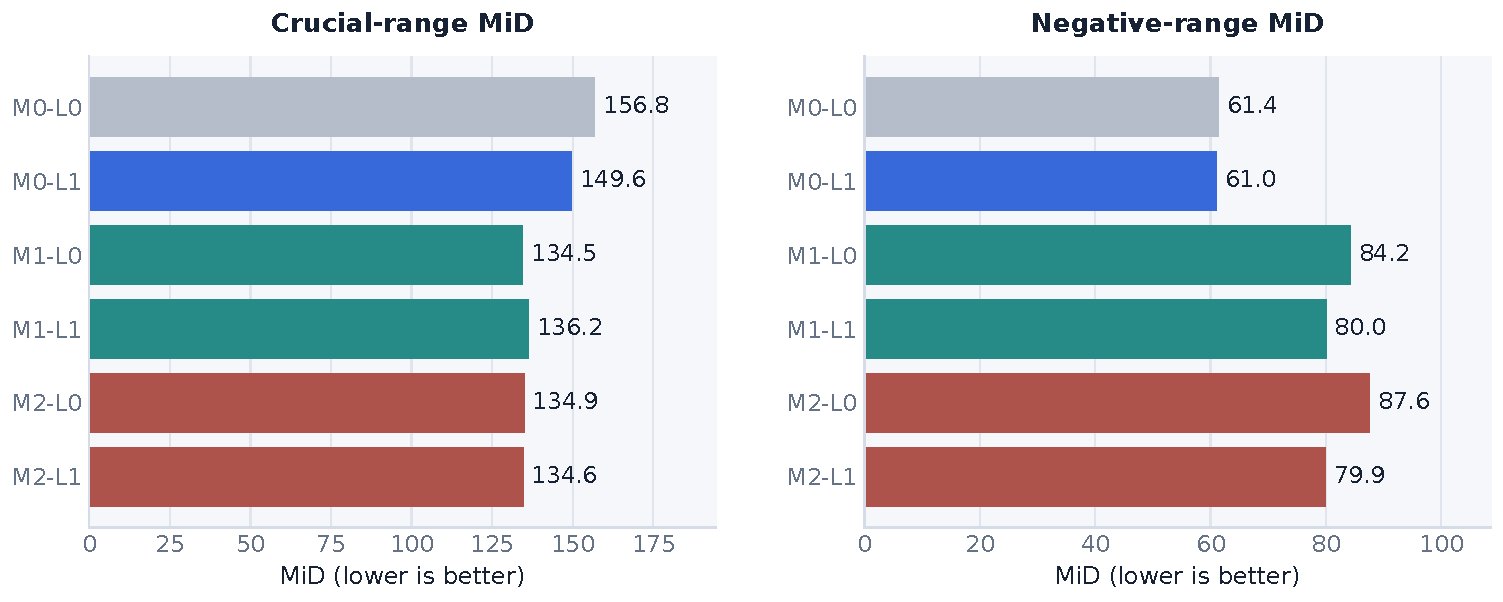
\includegraphics[width=0.98\linewidth]{figures/range_tradeoffs.pdf}
\caption{V14 MiD changes across crucial, small, large, and negative TTC bands.}
\end{figure}

\subsection{V15 and V17: testing readout and geometry explanations}

Neither readout intervention met the joint selection criteria. Sampling proportional to sample mass, corrected by $w_i/p_i$, preserved V14's cross-band tradeoff. Expanding the A5 residual range through an equal-slope hyperbolic tangent left crucial-band performance almost unchanged. The modified producer received regenerated PHASE17 fields and H normalizers.

V17 tested frozen geometry from several angles. A bypass exposed geometry and transport tokens to the temporal head; other arms examined learned NLL precision, grouped ridge probes, directional differences, height calibration and supervision, vertical position, gradient clipping, and nonlinear spatial-height readout. Each had a dedicated control. Directional differences remove static levels while also reducing dimensionality, so they do not isolate appearance memorization.

The geometry bypass carried a useful but unstable downstream signal. On V, its three-seed mean improved crucial MiD from 157.1 to 148.4 and aggregate MiD from 106.5 to 102.8, while MAE worsened. The effect was stronger on H than V, and the three heads shared encoders rather than repeating representation training.

The first height-regression arm emitted predictions outside the admissible MiD domain. Those invalid rows were retained, leaving the strict aggregate unavailable. Temporal supervision restored coverage but not competitive TTC accuracy. Preserving vertical positions improved training height fit while worsening H TTC, and the nonlinear readout also failed. The tested frozen-feature calibration was insufficient, though the bypass result still showed usable geometric signal.

Removing gradient clipping changed little. Learned precision improved crucial-band error in every head seed, but missed the required magnitude and safeguards. The recorded gradient norms describe one loss component rather than the full-dataset objective. None of V17's nine research lines produced a candidate. \evidence{L50,L51,L52}

\subsection{V18: adaptation of the measurement stage}

V18 moved adaptation into the measurement stage. Its primary comparison covered direct and correspondence-based pair readouts, trained and frozen encoders, and a native-system control. C1 tested geometric readout, D1 predictor width, B1 auxiliary correspondence supervision, and A1 adaptation depth. Some arms also updated correspondence, so equal TTC-update counts did not mean equal computation.

C1 improved bandwise geometry over an unconstrained pair-correction readout but failed as a complete TTC estimator. D1 found no benefit from greater predictor width. B1 beat a TTC-only control at the same number of TTC updates, yet its negative-band error blocked promotion over A5. A1 then compared full adaptation with partial retention of the correspondence-trained representation.

A1-FULL delivered V18's largest TTC gain and its clearest tradeoff. On H, aggregate MiD fell from 112.3 for A5-P2 to 78.9, and crucial MiD from 157.3 to 95.8; negative MiD rose from 65.5 to 87.1. It passed the global sign-error safeguard and beat last-block adaptation overall, but did not preserve accurate negative magnitude or demonstrate retention of the correspondence representation.

C1 also tested event information after the RGB context estimate. TRUE fusion and an equal-capacity ZERO-event control used seeds 7, 13, and 23. Each seed repeated C1 adaptation and head fitting, while all shared the historical A5 initialization and RGB context parent. The comparison isolates event input within this configuration, not variability from complete pretraining.

TRUE fusion improved on ZERO within V18. Across seeds, aggregate MiD was $87.3\pm0.9$ for TRUE and $92.5\pm0.2$ for ZERO; TRUE's crucial MiD was $126.6\pm0.9$. A paired whole-group bootstrap favored TRUE in aggregate loss. The crucial-band gain missed the preregistered 10\% threshold, and the interval against the preserved V16 PHASE-ONLY family crossed zero at about $[-3.7,0.1]$. Thus, events complemented RGB in this model without establishing superiority over V16.

No joint-measurement variant satisfied all accuracy and mechanism criteria. A later portability replay verified archived metrics and exports without adding training or performance evidence. \evidence{L10,L24,L25,L03,L31,L32,L33}

\begin{table}[tbp]
\centering\small
\caption{V18 primary and adaptive experiments on development subset H (18,422 rows). Sources \evidence{L10--L14,L20--L25}.}
\label{tab:late_v18}
\begin{tabular}{lrrrr}
\toprule
\textbf{Model} & \textbf{MiD} & \textbf{Crucial} & \textbf{Negative} & \textbf{MAE (s)} \\
\midrule
A5-P2-FROZEN & 112.29 & 157.27 & 65.52 & 5.64 \\
PAIR-DIRECT-S7 & 103.87 & 117.98 & 148.17 & 5.00 \\
PAIR-CORR-S7 & 103.51 & 115.56 & 156.00 & 5.50 \\
PAIR-CORR-FROZEN-S7 & 106.72 & 123.61 & 146.99 & 5.40 \\
NATIVE-P2-FT-S7 & 104.05 & 145.12 & 61.26 & 4.65 \\
PAIR-CORR-GEOMETRY-S7 & 90.95 & 114.35 & 106.23 & 6.95 \\
PAIR-CORR-WIDE-S7 & 115.12 & 124.48 & 206.42 & 6.79 \\
B1-TTC-CONTROL-STAGE2-S7 & 85.98 & 106.71 & 96.63 & 6.11 \\
B1-CORRESPONDENCE-STAGE2-S7 & 81.44 & 100.22 & 84.12 & 5.48 \\
A1-LAST-BLOCK-S7 & 90.64 & 111.03 & 97.96 & 7.11 \\
A1-FULL-S7 & 78.92 & 95.85 & 87.09 & 5.45 \\
\bottomrule
\end{tabular}
\end{table}
\begin{table}[tbp]
\centering\small
\caption{V18 C1 equal-capacity TRUE/ZERO event controls on exposed V (16,432 rows), using adaptation/head seeds 7, 13, and 23. Source \evidence{L03}.}
\label{tab:late-fusion}
\begin{tabular}{lrrr}
\toprule
\textbf{Head / seed} & \textbf{Overall MiD} & \textbf{Crucial MiD} & \textbf{MAE (s)} \\
\midrule
FUSION-TRUE-S7 & 88.270 & 127.661 & 1.817 \\
FUSION-ZERO-S7 & 92.638 & 136.989 & 1.842 \\
FUSION-TRUE-S13 & 86.630 & 125.976 & 1.807 \\
FUSION-ZERO-S13 & 92.455 & 136.500 & 1.837 \\
FUSION-TRUE-S23 & 86.961 & 126.069 & 1.818 \\
FUSION-ZERO-S23 & 92.315 & 136.314 & 1.836 \\
\bottomrule
\end{tabular}
\end{table}
\begin{figure}[t]
\centering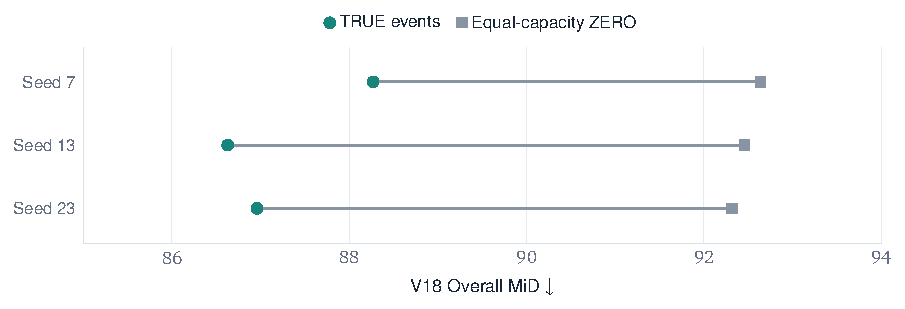
\includegraphics[width=0.98\linewidth]{figures/rev_v18.pdf}
\caption{V18 measurement adaptations and paired TRUE/ZERO event-fusion controls.}
\end{figure}

\subsection{V19: repairing negative motion changes the tradeoff}

V19 tested loss weighting as the source of A1's negative-band regression. L0 and LW shared the correspondence-trained B1 parent, full adaptation, seed 7, uniform sampling, and 12,000 updates. L0 assigned crucial/small/large/negative masses of 50/30/10/10\%. LW doubled negative mass to 20\% and set the positive bands to 44.44/26.67/8.89\%, preserving their relative proportions. Both arms kept the same encoder architecture and B1 initialization, while FULL adaptation updated encoder and readout weights; only the loss-band masses differed between arms. The training implementation requires a nonzero encoder-weight change after updates. \evidence{P03}

\begin{table}[tbp]
\centering\small
\caption{V19 decision recovery on exposed H. LW trades a small overall MiD increase against improved MAE and negative-range behavior. Source \evidence{L30}.}
\label{tab:late_v19}
\begin{tabular}{lrrrr}
\toprule
\textbf{Model} & \textbf{MiD} & \textbf{Crucial} & \textbf{Negative} & \textbf{MAE (s)} \\
\midrule
A5 & 112.29 & 157.27 & 65.52 & 5.64 \\
L0 & 78.92 & 95.85 & 87.09 & 5.45 \\
LW & 79.87 & 100.42 & 70.78 & 4.61 \\
\bottomrule
\end{tabular}
\end{table}

LW repaired part of the negative-motion error but worsened the primary aggregate. Relative to L0, it reduced negative MiD by 18.7\%, MAE by 15.3\%, and sign error by 1.55 percentage points, while aggregate and crucial MiD increased. The same pattern appeared on P training data, ruling out an H-only generalization failure. Because the replication trigger required lower aggregate error, LW did not advance.

Later two-expert selectors also did not meet the system-level selection criteria. They required both fitted experts and the measured feature path, rather than forming a jointly trained sparse mixture. Grouped validation limited fitting leakage, while reused H data and fixed experts constrained the conclusion to these selectors.
\evidence{L30}
\FloatBarrier

\section{Representation and physical-measurement follow-ups}
\label{app:physics-followup}
The new experiments extend the historical controls with narrower questions: whether future-state prediction preserves useful expansion increments, whether a scalar motion quantity is observable under the fitted model, and whether a sensor or clock residual predicts a better TTC estimate. Each experiment retains its own population and reference model. An improvement in an auxiliary metric does not substitute for a TTC comparison. \evidence{N04,N05}

\subsection{A closed predictive-learning pilot}
The event student learns against spatial features from a frozen, distilled V-JEPA~2.1 ViT-B teacher~\citep{vjepa21}. For each of seeds 7, 13, and 21, the pilot runs static distillation, one-step prediction, and a cross-sequence shuffled-future control for 1,000 updates with batch size 16. TTC labels do not enter these student losses. The final checkpoint is fixed before evaluation. After training, a ridge probe with regularization parameter one reads temporal differences of the frozen encoder, with the predictor removed. It fits on 512 P samples from twenty-four sequences and evaluates 256 H samples from eight different sequences. Box-based localization remains privileged information. \evidence{N04}

The primary target is annotated log-height change. Its error is dimensionless: it is neither a time-normalized rate nor TTC error in seconds. The criterion requires the one-step arm to beat both static distillation and shuffled futures, with the upper endpoint of each sequence-bootstrap difference interval below zero. The bootstrap resamples eight complete sequences while keeping the three seeds together, so its interval remains conditional on those seeds and on historically exposed H sequences.

\EvidenceJepaTable
The candidate's probe MAE is 0.03564004, compared with 0.03763239 for static distillation and 0.03506189 for shuffled futures. Its candidate-minus-static difference is $-0.00199235$, with interval $[-0.00496210,0.00081898]$; candidate-minus-shuffled is $0.00057816$, with interval $[-0.00217005,0.00292590]$. Neither superiority criterion passes. The random-initialization control gives 0.03719641. This failed continuation criterion is not an equivalence test or evidence that predictive learning can never help.

The auxiliary latent metrics clarify the limitation. Future teacher-state MSE improves relative to both controls, but teacher-increment MSE worsens. The corresponding candidate-minus-static changes are $-0.01719163$ for state and $+0.03848016$ for increment; candidate-minus-shuffled changes are $-0.05317388$ and $+0.00447422$. Predicting a future state can compensate for present-state errors or model variation irrelevant to expansion, but the experiment does not identify either explanation causally. Its results establish that lower state-prediction error was insufficient for the prescribed physical probe. The pilot closed without rollout, scaling, or integration into the released estimator. \evidence{N04}

\subsection{Target-specific observability and model error}
For a linearized observation model $\mathbf y=H\boldsymbol\beta+\boldsymbol\epsilon$ and target $q=\mathbf c^\top\boldsymbol\beta$, noiseless identifiability requires $\mathbf c$ to lie in the row space of $H$. In the affine image-motion parameterization, isotropic expansion uses $\mathbf c=(1/2,0,0,1/2,0,0)^\top$. The target can be estimable without every affine coefficient being identifiable. Conversely, a pseudoinverse always returning a number does not certify that the target is supported. This algebraic condition is classical and is used here as a diagnostic. \evidence{N05}

On the 149-query screen, the diagnostic marks $q$ estimable in 63 queries. Among those estimates, 26 have an incorrect sign, ten lie outside the canonical phase domain, and eight have zero residual degrees of freedom. A small fitted residual in the last group cannot demonstrate reliability. The target itself also need not equal local isotropic image expansion when rotation, parallax, or changing visible surfaces violate the measurement model.

The gain-prediction experiment compares physical descriptors against simpler support descriptors with leave-one-acquisition-out fitting. Physical-feature MSE is 0.919267453, versus 0.492043720 for support features; their difference is 0.427223732 with interval $[0.080550690,1.010417232]$. This is MSE for predicting correction gain, not TTC MAE. The result rejects the proposed descriptor gate. A historical robust readout returns only eight usable estimates, four with the wrong sign; after preserving F0 fallback, its MAE is 0.779543461\,s versus 0.766024827\,s for the matched R0 baseline. The comparison records unavailable measurements and the original missing output; the error of the eight supported measurements is not presented as complete-population performance. \evidence{N05}

\subsection{Sensor ambiguity and the missing reference}
The sensor-identifiability bank constructs 24 pairs of matching event streams, with pixel, polarity, and timestamp agreement to a tolerance of one picosecond. Twelve pairs have different inverse TTC. Under the bank's log-affine texture model, changing motion and inversely scaling the texture gradient can preserve the increments that generate events; the distinct initial references are absent from the event stream. Providing a known reference helps distinguish the restricted conditions. This construction diagnoses an ambiguity in the tested model, not a general impossibility theorem for event-based estimation. \evidence{N05}

The real-data proxy uses 72 road queries from twenty-four acquisitions. Slider is excluded from the photometric fit because its alignment remains provisional. On common support, observed RGB change gives sensor-residual MSE 96.657290 versus 145.648563 for the physical proxy. Its improvement over an activity control is less decisive: the corresponding descriptive difference interval includes zero. Sensor-residual reductions cannot be interpreted as TTC improvements, and the inventory does not establish calibrated contrast thresholds, gain, initial reference, or refractory response.

The direct rate readout tests that implication. The affine photometric model permits translation, deformation, and global illumination variation and returns 72 valid rate estimates. With the original fallback retained, its macro TTC MAE is 9.168523738\,s, compared with 0.766024827\,s for R0. The spatially permuted control is worse still, at 45.629594312\,s. Beating that control is insufficient when the matched estimator deteriorates so strongly. The experiment opens no producer or JEPA training and supplies no calibrated confidence signal for fusion. \evidence{N05}

\subsection{Surfaces and dynamic clocks}
For positive depth $Z$, signed inverse TTC is $q=-\dot Z/Z$. Differentiation gives
\begin{equation}
 \dot q=q^2-\ddot Z/Z.
\end{equation}
If axial relative velocity is constant in this coordinate, its finite-time evolution is
\begin{equation}
 q(t+\delta)=\frac{q(t)}{1-\delta q(t)},\qquad T(t+\delta)=T(t)-\delta.
\end{equation}
The transport cannot cross the contact singularity. Acceleration, camera rotation,
or a change in the visible surface can invalidate the assumptions even when an
object has constant velocity in world coordinates. These relations follow from
kinematics; the experiment tests their utility in the estimator rather than
claiming a new physical law. \evidence{N05}

A three-frame surface route supplies 133 of 149 measurements and falls back on the other sixteen. Its system MAE is 3.103982972\,s versus R0's 0.766024827\,s, with a paired difference interval $[0.934231309,4.198244944]$\,s. The crop audit finds no changing crop within the 146 auditable histories; 53 contain a constant anisotropic resize. This rules out one proposed changing-zoom explanation for that cohort, not errors from occlusion, backgrounds, or parallax. \evidence{N05}

The constant-axial-velocity transport law above is exact only under its model assumptions. Reapplying its composition identity inside an exact implementation adds no new measurement. The follow-up compares fixed persistence, smoothing, transport, and observer rules against their matched event context after canonical PAIR. Context macro MAE is 1.941890262\,s; EWMA gives 1.952822072\,s, the observer 1.981365164\,s, and persistence/transport 3.104231759\,s. These comparisons do not establish a benefit. Their baseline is the event context, which must remain distinct from the multimodal R0 baseline used above. \evidence{N05}

Together, these experiments distinguish implementation correctness, model identifiability, and useful downstream prediction. No rejected gate becomes a successful learned physical model because its equations are interpretable. Further training would require a new, bounded hypothesis supported by these failures and evaluated with appropriate controls; it is not a result already achieved by this revision.
\FloatBarrier

\section{Detection, geometric consistency, and the localization boundary}
\label{app:detection-followup}

The TTC evaluations in this paper condition on supplied object regions. A separate eAP study develops a portable RGB MonoDGP-R50 variant, a proposal ranker, and an interface from tracked detections to PHASE-TTC. We report this work to examine the localization dependency. Its detection scores, geometric diagnostics, and integration checks do not establish improved end-to-end TTC accuracy. The detector is also distinct from the event representation and predictive-learning experiments. \evidence{N06}

\subsection{Fixed proposals and an aligned evaluator}
On 23,958 development-exposed frames, the aligned eight-class evaluator gives mAP 0.05701726 for the retained Dfull detector and 0.06204229 after a TRAIN-fitted shared logistic ranker. Both evaluations use the same 1,197,900 proposals and 190,469 raw targets. Ranking changes the scores while preserving proposal geometry, classes, and velocities. Bicycle and other-vehicle AP remain zero; the aggregate gain does not imply uniform class improvement. The study uses one detector seed and a selection population reused during development. \evidence{N06}

Evaluation reconciliation matters here. Earlier AP101 reports used a restricted target population and a precision envelope. The aligned calculation uses greedy class matching in ego-XY coordinates, strict distance thresholds of 0.5, 1, 2, and 4\,m, recall interpolation without the envelope, and the declared minimum-recall and minimum-precision rules. The two calculations are different estimands. We retain their historical records rather than comparing their numeric magnitudes as model improvements. The ranked submission obtains official AP 0.05129508 on 35,940 test frames; no paired baseline submission exists, so the local ranking gain cannot be transferred to the official test. \evidence{N06}

\subsection{Ideal cuboid inversion and predicted geometry}
The geometric audit asks whether a height-only depth prior has a bias even with ideal inputs. Let $\boldsymbol\delta_i$ be a rotated cuboid-corner offset, $\mathbf u$ the projected center, and $K$ the camera intrinsic matrix. Define
\begin{equation}
 \mathbf a_i=K_{1:2,:}\boldsymbol\delta_i-\mathbf u\delta_{iz}.
\end{equation}
For a positive center-to-edge distance $t_e$, cuboid containment gives
\begin{equation}
 z_e=\max_i\left(\frac{s_e(\mathbf a_i)}{t_e}-\delta_{iz}\right),
\end{equation}
where $s_e$ selects the signed horizontal or vertical numerator for that edge. The implementation takes a median over non-clipped edges; a clipped image boundary is not treated as an equality. This is a pinhole consistency calculation, not a new physical law. \evidence{N06}

With target-derived dimensions, yaw, and projected edges, the admitted set contains 25,424 objects from 4,096 TRAIN frames. On the same admitted objects, the height prior has depth MAE 4.923050\,m, whereas cuboid-edge inversion reaches $2.1085\times10^{-6}$\,m. The near-zero error verifies consistency with the ideal target generator. It does not measure sensor calibration or learned depth accuracy. \evidence{N06}

A second experiment substitutes predicted geometry on a \emph{different} 4,096-frame TRAIN panel. It preserves the proposal pool, class, score, size, and yaw, but replaces the learned depth output and removes its learned residual. Baseline mAP 0.21064779 falls to 0.16478485 with cuboid-edge depth and to 0.08308035 with the height-only prior. Invalid geometric cases use the declared fallback. Thus the better ideal inversion does not improve this direct substitution. No model is promoted, and the experiment does not rule out retraining a compatible residual or estimator. \evidence{N06}

\subsection{Negative screens and integration scope}
The later range, class-budget, query-ranking, KITTI-transfer, and MonoCoP campaigns do not justify replacing the retained detector. Short, single-seed screens and differing upstream training exposure restrict their interpretation; they are not evidence that every related architecture or transfer recipe must fail. The unpromoted candidates remain in the experimental record. \evidence{N06}

An eight-frame integration replay produces five available signed TTC outputs and one unconfirmed track in the last frame. This demonstrates execution of the detector--tracker--TTC interface. Frozen TRAIN40 producers had already seen these sequences, and the replay supplies no independent end-to-end TTC accuracy estimate. The admission protocol also distinguishes target time from availability: the target is anchored at RGB exposure start, while inference can consume observations through exposure end. The resulting estimate has a measured availability lag and must not be described as causal at the earlier target instant. These boundaries remain necessary when replacing supplied boxes with predictions. \evidence{N06}
\FloatBarrier

\section{Experimental chronology}
\label{sec:history}

Development began in June 2026 with the E-JEPA-TTC hypothesis: predictive latent
learning might improve event-based TTC estimation. The research then moved
through geometry and cross-time transport to temporal context and RGB--event
fusion. Several evaluation corrections changed which results could support a
claim.

\subsection{June--July: predictive learning and evaluation corrections}

The first experiments established indexed EvTTC access, voxel representations,
a TinyCNN, and geometric/event-rate baselines. JEPA pretraining with
latent-variance regularization led to multihorizon prediction, frozen-encoder
probes, and low-label comparisons. Token transformers, tubelets, deep token
supervision, navigation conditioning, and rollout probes tested other forms of
temporal information.

Centered derivatives gave the geometric baseline access to future observations.
I replaced them with past-only derivatives and reported this annotation-assisted
baseline on its supported queries, separate from models with different inputs or
coverage.

On 13 July, I reclassified the inspected CPLA-high results as reused-test
diagnostics (\texttt{26480260}). Their three fine-tuning seeds shared one SSL
initialization, so the spread reflects downstream optimization conditional on
that parent. I removed the runs from final-test claims and added checkpoint,
cache-version, nested-subset, and matched-scratch checks. No repartition of the
inspected sequences could recreate a blind holdout.

An eAP smoke-validation defect wrote success markers without running the matrix
(\texttt{1f9e2f99}). I replaced the faulty path with the matrix invocation and
added a regression test; the old markers were discarded as evidence.

\subsection{August: geometry, transport and fold-local parents}

August introduced physics-constrained FlowMimic, dense LevelDynamics,
object-centric representations, and matched Garl comparisons. The A-series
varied foreground geometry and decoder capacity, then added SAM supervision and
DINOv3 relational distillation. A4 used an RGB teacher; A5 learned local
cross-time transport on disjoint training rows. These stages no longer tested
the original label-free JEPA objective alone.

On 13 August, I found that several grouped runs inherited an A4 parent trained
on their held-out outer groups (\texttt{de3349fd}). Those summaries remain
parent-exposed diagnostics. The corrected study trained A4 inside each outer
fold, keeping the held-out group out of both representation learning and
downstream fitting.

V6 and V7 produced no promoted model. A post-hoc A5/C2F routing result from V7
became a prospective V8 hypothesis. V8 then tested temporal mechanisms and
nested routing after correcting ROI quantization, timestamp bins, and bounded
HDF5 reads. Unsupported predictions stayed in the evaluation as named failures.

\subsection{September--October: context and multimodal measurement}

X0/X1 and Stages 61--76 tested phase dynamics, raw timing, routing, risk, and
context under fixed optimization budgets. Nested producers excluded held-out
groups from training, and incomplete runs were not promoted to completed
evaluations.

SIMPLEX-T completed 24 head fits and 60,000 updates. Its H8/H16 comparisons
retrained heads while sharing upstream producers. Efficient-context work then
addressed TRAIN40 inputs and execution cost; the RGB port added native sensor
clocks and transfer studies. The record also retains failed geometry, clipping,
and nonlinear-readout controls from the range and representation studies.

The multimodal V16 phase-correction family supplied the final-refit recipe.
V18 tested joint measurement, correspondence, geometric readout, predictor
capacity, and encoder adaptation. Some arms improved individual bands, but none
passed every promotion criterion; V18 closed as \texttt{NO\_CANDIDATE}. V19
then tested negative-loss weighting and fixed expert selection.

\subsection{October: final refit and causal runtime}

The final TRAIN40 refit used group-separated auxiliary producers for
out-of-fold inputs and full-TRAIN40 producers for deployment. It followed the
V16 recipe but trained a new model lineage. The submission preserved query-token
identity and complete prediction coverage, and its official score placed
PHASE-TTC first on the public GarlTTC Test leaderboard on 28 October 2026
(Section~\ref{sec:official}).

Runtime experiments covered persistent histories, exact normalization, graph
execution, crop reuse, and multiobject replay. Timing reports separated startup
from measured arrivals and counted valid TTC outputs separately from failed acknowledgements.
The 5\,ms ingestion experiment kept 20\,ms output queries and established
numerical parity for that setting; it did not measure throughput.

\subsection{29 October--2 November: adaptation and controlled follow-ups}
The subsequent work recovered target correspondence for all 434 EvTTC queries, fitted a compact quality adapter over frozen TRAIN40 components, and tested canonical elapsed-time handling. The delivered adapter and the later rejected canonical refits remain distinct. Physical-measurement and fixed-teacher predictive-learning experiments produced negative controls; a separate eAP detection branch investigated localization, evaluation alignment and geometric priors. Sections~\ref{sec:quality-adaptation} and~\ref{sec:canonical-cadence}, together with Appendices~\ref{app:physics-followup} and~\ref{app:detection-followup}, describe these additions with their own evidence and exposure histories.

\section{Open science and reproducibility}
\label{app:reproduction}

The manuscript sources, analysis scripts, result ledgers, and selected query-level predictions are available in \href{https://github.com/Kripta-Studios/phase-ttc}{Kripta-Studios/phase-ttc}. The source package supports regeneration of the reported tables and figures. Repeating training or sensor inference additionally requires the datasets, checkpoints, and configurations identified in the evidence registry.

\subsection{Manuscript and result regeneration}
Install Python with NumPy, Matplotlib, Pillow, and PyMuPDF, together with pdfLaTeX and BibTeX. From the manuscript source root, run:
\begin{lstlisting}
python scripts/build_expanded.py
python scripts/verify_publication.py
\end{lstlisting}
The builder verifies the distributed inputs, preserves historical figures, regenerates the expanded result tables, and compiles both modular and consolidated sources. After dependency installation, this process uses bundled data without network access or raw sensor files. A publication receipt binds the scientific inputs, compiled PDF, consolidated source, and build validation by SHA-256. Packaging rejects changed inputs or artifacts until the manuscript is rebuilt. Earlier editorial receipts identify their historical PDF hashes and do not validate the corrected delivery.

Each result ledger identifies its evaluation population and measured quantities. Verification scripts recompute the distributed query-level metrics and check their source identities. Hardware-specific parity requires the corresponding inputs, checkpoints, and runtime environment.

\subsection{Numerical and software verification}
The source checks cover thirteen data-file hashes, eight transfer summaries, twelve official-scorer fields, and weighted Overall MiD. The competition verifier recomputes coverage, signed ranges, disagreement, and timing summaries across 1,736 model--query rows. Official scores reconcile with the dated leaderboard after rounding.

\begin{table}[H]
\centering\small
\caption{Additive decomposition of the official Overall MiD difference. Each band contributes $w_b(\mathrm{MiD}^{\mathrm{Garl}}_b-\mathrm{MiD}^{\mathrm{PHASE}}_b)$. The 0.0010-point reconciliation residual comes from Garl-TTC's published two-decimal band scores and appears separately below. \evidence{B01,B02}}
\label{tab:official-weighted-contributions}
\begin{tabular}{lrrr}
\toprule
\textbf{Band} & \textbf{Weight} & \textbf{MiD difference} & \textbf{Weighted contribution} \\
\midrule
Crucial & 0.5 & 9.6110 & 4.8055 \\
Small & 0.3 & 9.3232 & 2.7970 \\
Large & 0.1 & 14.8921 & 1.4892 \\
Negative & 0.1 & 1.3586 & 0.1359 \\
\midrule
Band subtotal & 1.0 & -- & 9.227548419 \\ 
Published-score rounding residual & -- & -- & 0.0010 \\ 
Official Overall difference & -- & -- & 9.228548419 \\ 
\bottomrule
\end{tabular}
\end{table}


The historical transfer analysis under \path{revision/} uses 468 eligible Extended-new rows under the original target-source assignment. Correcting the CCRs1 low/medium sources and recomputing eligibility yields 460 eligible rows from the same 508 candidates; the corrected analysis and source map are retained separately under \path{audit_20261104/}. Both analyses retain the saved predictions and use complete sequence groups for paired bootstrap resampling. Their fixed seed, quantile convention, paired differences, and source digests distinguish corrected analysis from the historical snapshot.

The recorded software checks cover event representations, target updates, causal prefixes, label rejection, source tracking, fusion fallbacks, and paced-runtime accounting. With Python 3.11.15, PyTorch 2.11.0+cu128, and pytest 9.1.1, two batches passed 178 tests with four skips. The original M21 XML receipts record 70 cases with four skips and 112 cases without skips, respectively, with no errors or failures; the corresponding logs and XML files are distributed as \path{data/verification_architecture.*} and \path{data/verification_protocol.*}. These files retain the SHA-256 identities in the architecture source index and report the historical runs of 28 October 2026. Rebuilding the paper does not rerun these tests. Four further tests passed against the fixed official evaluator, covering four-band perfect predictions, imminent-contact weighting, missing bands, and invalid outputs. \evidence{M21,M24}

The competition adapter and verifier passed 41 focused tests; the CPU suite skipped one CUDA-dependent case. A separate CUDA check confirmed strict loading and native-model forward parity for all three public Garl checkpoints. Validation also checked the 1,302 Garl outputs, 434 PHASE predictions, query identities, input timing, signed height-ratio conversion, and result completeness. These are the archived execution results, separate from rebuilding the manuscript. \evidence{M21,M24,T01}

\subsection{Source revisions and methodological corrections}
Table~\ref{tab:source-revisions} centralizes code revisions associated with the scientific record. The evidence registry identifies 95 original result snapshots by SHA-256 and records their available numerical projections. Entries containing only source identity require the corresponding original artifacts for metric recomputation. The archived scorer JSON and public leaderboard identify the official result; the scorer JSON does not contain a submitted-prediction digest.

\begin{table}[H]
\centering\footnotesize
\caption{Source revisions for reproduction and protocol corrections. Historical identifiers remain unchanged in the repository.}
\label{tab:source-revisions}
\begin{tabularx}{\linewidth}{@{}p{.36\linewidth}X@{}}
\toprule
Scope & Git revision \\\midrule
Scientific source snapshot & \path{0219a84f0fc3b07c171295a8a65176a7e0f631c1} \\
Competition adapter & \path{1d8de7d95b2ff8ccba884dbd40141c48745a1e95} \\
CPLA-high exposure classification & \texttt{26480260} \\
Evaluation-matrix execution correction & \texttt{1f9e2f99} \\
Fold-specific producer correction & \texttt{de3349fd} \\
\bottomrule
\end{tabularx}
\end{table}

The competition projection includes predictions, measurement boundaries, checkpoint identities, and source digests for coverage, disagreement, and timing analysis. Raw sensor data remain subject to their dataset distribution terms. \path{ASSETS.md} records image attribution and display transformations; \path{data/real_sensor_excerpt/} preserves the real sensor excerpt's provenance, timestamps, and original asset hashes.

\subsection{Runtime configuration}
The L40 receipts specify the final component identities and the separate paced-replay input and clock. Model loading, synthetic shape priming, and history initialization precede measured arrivals; unexpected preparation during updates remains in latency. The records identify the laptop GPU and execution settings but omit the CPU model and GPU-driver version. \evidence{L40,R02}
\begin{table}[H]\centering\small
\caption{Paced-replay hardware, configuration, and initialization timings. Startup stages were timed separately and excluded from the arrival clock; unexpected shapes were processed within the measured update. \evidence{L40,R02}}
\label{tab:runtime-setup}
\begin{tabularx}{\linewidth}{@{}p{.31\linewidth}X@{}}\toprule
Item & Recorded value\\\midrule
GPU & NVIDIA GeForce RTX 5070 Ti Laptop GPU\\
Software & Python 3.11.15; PyTorch 2.11.0+cu128; CUDA build 12.8\\
Precision & FP32; TF32 disabled for matrix multiplication and cuDNN\\
CPU / preparation & 2 PyTorch CPU threads; 8 RGB workers; queue capacity 2\\
Parity tolerance & Absolute and relative tolerance both $10^{-5}$; all 250 outputs checked\\
\midrule\multicolumn{2}{l}{\textbf{Outside the measured arrival clock}}\\
RAW preload & 2.769 s\\
Model and service initialization & 0.516 s\\
Synthetic shape priming & 12.095 s; 7 layouts; synthetic tensors only, no RAW/future sensor data\\
History initialization & 0.132 s for 600 ms of preceding sensor history\\
Source warmup & 0.051 s; 13 already-available RGB frames\\
\midrule
Unrecorded hardware fields & CPU model and GPU driver version\\
\bottomrule\end{tabularx}\end{table}


\subsection{Expanded edition}
The expanded result tables regenerate from the copied JSON ledgers under \path{updates/}. The build preserves original sections and figures, updates conclusions where later measurements supersede them, and includes the source index in Appendix~\ref{app:update-evidence}. Rebuilding the document reuses recorded model outputs. The source manifest binds the final manuscript, figures, ledgers, and validation receipts; the source ZIP includes the assets needed to compile the consolidated \LaTeX{} file.

\section{Evidence index}
\label{app:evidence}
Source keys map each reported measurement to its result artifact. Numerical ledgers drive table and figure regeneration, while \path{data/public_evidence_registry.json} records full digests and field selectors. The index separates original-artifact hashes from distributed-file hashes. \emph{Digest only} entries preserve source identity without distributing the fields required for metric recomputation. B02 denotes the official scorer JSON.
\subsection{Result-source identities}
\begingroup\footnotesize
\setlength{\tabcolsep}{3pt}
\renewcommand{\arraystretch}{1.08}
\begin{longtable}{@{}>{\raggedright\arraybackslash}p{.32\linewidth}>{\raggedright\arraybackslash}p{.41\linewidth}>{\raggedright\arraybackslash}p{.22\linewidth}@{}}
\toprule
Source key & Distributed ledger & Original SHA-256 \\
\midrule\endfirsthead
\toprule
Source key & Distributed ledger & Original SHA-256 \\
\midrule\endhead
\midrule\multicolumn{3}{r}{\scriptsize Continued on next page}\\\endfoot
\bottomrule\endlastfoot
\path{E01} & \path{data/early_results.json} & \path{55b5494b40f97f1b} \\
\path{E02} & \path{data/early_results.json} & \path{27ee1c9a21cca0ec} \\
\path{E03} & \path{data/early_results.json} & \path{aa46f6d199bcf5a4} \\
\path{E04} & \path{data/early_results.json} & \path{02c215aa4678f307} \\
\path{E05} & \emph{Digest only} & \path{6fe8c8761d0a14fb} \\
\path{E06} & \emph{Digest only} & \path{d38021db5b3b5b62} \\
\path{E07} & \path{data/early_results.json} & \path{d53b6ce406fa7b80} \\
\path{E08} & \path{data/early_results.json} & \path{d69f8b9082c883da} \\
\path{E09} & \path{data/early_results.json} & \path{9bf197c3d64635a3} \\
\path{E10} & \path{data/early_results.json} & \path{d47face1e36d1d2c} \\
\path{E11} & \path{data/early_results.json} & \path{6db419fd7c7fe536} \\
\path{E12} & \path{data/early_results.json} & \path{f33dc9abbad8fd08} \\
\path{E13} & \emph{Digest only} & \path{ac26c1b2ad87c6c9} \\
\path{E14} & \emph{Digest only} & \path{f947b32f05e655a1} \\
\path{E15} & \emph{Digest only} & \path{7c60bc0fa9f1c5f0} \\
\path{E16} & \path{data/early_results.json} & \path{be5fdbc0b2e9773d} \\
\path{E17} & \path{data/early_results.json} & \path{d3fb5a5feb848ac7} \\
\path{E18} & \path{data/early_results.json} & \path{a3c4765f5278a3f4} \\
\path{E19} & \path{data/early_results.json} & \path{f1471599d502f2de} \\
\path{E20} & \path{data/early_results.json} & \path{3e02fd81751e3f86} \\
\path{E21} & \path{data/early_results.json} & \path{5c7b1eb24c07bd08} \\
\path{E22} & \emph{Digest only} & \path{2e2eef6698ef28a4} \\
\path{E23} & \path{data/early_results.json} & \path{bc540cc21ddb317f} \\
\path{E24} & \emph{Digest only} & \path{dab563a02450abe6} \\
\path{E25} & \path{data/early_results.json} & \path{06619299d1ceb785} \\
\path{E26} & \path{data/early_results.json} & \path{06dc45cf3ea7a3e0} \\
\path{M_SIMPLEX} & \path{data/middle_results.json} & \path{93f83e71f86dfcad} \\
\path{M_HEAD_COST} & \path{data/middle_results.json} & \path{8d96bbc9bd66d8fb} \\
\path{M_ROUTE_COST} & \path{data/middle_results.json} & \path{d1d834ab36d14fbd} \\
\path{M_WIDE} & \emph{Digest only} & \path{c15e32a8dea0eece} \\
\path{M_EWMA} & \emph{Digest only} & \path{47cca03ccda6f054} \\
\path{M_STAGE61} & \path{data/middle_results.json} & \path{20f1990bb70e5de7} \\
\path{M_STAGE62} & \path{data/middle_results.json} & \path{c4a0e1ae20d79094} \\
\path{M_GEOMETRY} & \emph{Digest only} & \path{fa917902b5696e4b} \\
\path{M_STAGE67_DECISION} & \emph{Digest only} & \path{ab1d3095955477f4} \\
\path{M_STAGE69_DECISION} & \emph{Digest only} & \path{dfd1956775492584} \\
\path{M_ENGINEERING} & \emph{Digest only} & \path{e756ba5c7a433efd} \\
\path{M_SCIENCE_AUDIT} & \emph{Digest only} & \path{06073f4182de1a41} \\
\path{M_STAGE63_REPAIR} & \emph{Digest only} & \path{f96b7fe795637cc5} \\
\path{M_CAPACITY_PROTOCOL} & \emph{Digest only} & \path{1be3a4c9f9b64a08} \\
\path{M_CAPACITY_AUDIT} & \emph{Digest only} & \path{07ef97a56b4159fa} \\
\path{M_STAGE70_LEDGER} & \emph{Digest only} & \path{62597e162571def0} \\
\path{M_TRANSFER_REPORT} & \emph{Digest only} & \path{d92c9074516354bd} \\
\path{M_ROUTE_REPORT} & \emph{Digest only} & \path{1f29a459c91f6b68} \\
\path{M_TEMPORAL_MODEL} & \emph{Digest only} & \path{4c26ad5ecf9e8354} \\
\path{M_PHASE_CONTRACT} & \emph{Digest only} & \path{7ee447190ef7b218} \\
\path{M_STAGE64} & \emph{Digest only} & \path{68409fb88499899f} \\
\path{M_X0} & \emph{Digest only} & \path{61d8a0e40b6d87ad} \\
\path{M_X05} & \emph{Digest only} & \path{c4aa55dd6a944d01} \\
\path{M_X05_GATE} & \emph{Digest only} & \path{61eae7d38fb6ea5a} \\
\path{M_STAGE65} & \emph{Digest only} & \path{4f88f676eecc7e90} \\
\path{M_STAGE67_DIAGNOSTICS} & \emph{Digest only} & \path{885ac3604160cf27} \\
\path{M_S67_SIMPLEX17} & \emph{Digest only} & \path{969cf5db29b2a251} \\
\path{M_S67_UNCONSTRAINED17} & \emph{Digest only} & \path{1419522be60fc952} \\
\path{M_S67_SIMPLEX8GATE} & \emph{Digest only} & \path{e094512164179869} \\
\path{M_S67_SIMPLEX17_PAIRPERM} & \emph{Digest only} & \path{451821bb98c1d0c2} \\
\path{M_S65_RISK17} & \emph{Digest only} & \path{b964e12180efbcbc} \\
\path{M_S65_RISK8} & \emph{Digest only} & \path{75d98c9e0be9ddc3} \\
\path{M_V12_EVTTC_946} & \path{data/middle_results.json} & \path{03c57b4503ca95f4} \\
\path{M_V12_EVTTC_946_PAIRED} & \emph{Digest only} & \path{5fee507ffe8a4aca} \\
\path{M_V12_EVTTC_946_ROWS} & \emph{Digest only} & \path{d284e52a0c25a897} \\
\path{M_V12_EVTTC_3640} & \path{data/middle_results.json} & \path{792a5042dfa8be8b} \\
\path{M_V12_EVTTC_3640_PAIRED} & \emph{Digest only} & \path{2619cc3d11be7320} \\
\path{M_V12_EVTTC_3640_ROWS} & \emph{Digest only} & \path{20f58c1200b3834d} \\
\path{M_V12_FCWD_597} & \path{data/middle_results.json} & \path{a1c0c4a741b08a36} \\
\path{M_V12_FCWD_597_PAIRED} & \emph{Digest only} & \path{2581bd042f29a466} \\
\path{M_V12_FCWD_597_ROWS} & \emph{Digest only} & \path{68f4cd5610f50c8b} \\
\path{L01} & \path{data/late_results.json} & \path{9136babd4a07411e} \\
\path{L02} & \path{data/late_results.json} & \path{844e0771bab79717} \\
\path{L03} & \path{data/late_results.json} & \path{4af996900a99c585} \\
\path{L10} & \path{data/late_results.json} & \path{f5bf12b2873a2ee4} \\
\path{L11} & \path{data/late_results.json} & \path{22e82a376b18c9f0} \\
\path{L12} & \path{data/late_results.json} & \path{fafd9cefbeddcd49} \\
\path{L13} & \path{data/late_results.json} & \path{86ce201ca25bcc12} \\
\path{L14} & \path{data/late_results.json} & \path{0588956e96dab44f} \\
\path{L20} & \path{data/late_results.json} & \path{6d15d1acfad38592} \\
\path{L21} & \path{data/late_results.json} & \path{2b33ba213186f3c5} \\
\path{L22} & \path{data/late_results.json} & \path{b1ad71b126b20e87} \\
\path{L23} & \path{data/late_results.json} & \path{0698e433731da0d3} \\
\path{L24} & \path{data/late_results.json} & \path{5f3789bd7efebce3} \\
\path{L25} & \path{data/late_results.json} & \path{774c751e4aaa91d7} \\
\path{L30} & \path{data/late_results.json} & \path{1073ab21e307ae26} \\
\path{L31} & \path{data/late_results.json} & \path{54ebca7a19d5a9eb} \\
\path{L32} & \path{data/late_results.json} & \path{d4fbc7494769a5d1} \\
\path{L33} & \path{data/late_results.json} & \path{025a058d846a7ceb} \\
\path{L40} & \path{data/late_results.json} & \path{c27d5d980f2bb1c1} \\
\path{L41} & \emph{Digest only} & \path{d8df9ca6444c6dc0} \\
\path{L42} & \emph{Digest only} & \path{06ab49e521db7255} \\
\path{L43} & \emph{Digest only} & \path{aed0bdd40c58d827} \\
\path{L44} & \emph{Digest only} & \path{e447c5147e4e1c25} \\
\path{L45} & \emph{Digest only} & \path{4f643a15cbf3d963} \\
\path{L46} & \path{data/transfer_queries.csv} & \path{1fbff40f000c879b} \\
\path{L50} & \emph{Digest only} & \path{3069072fb5180272} \\
\path{L51} & \emph{Digest only} & \path{ad4a2a0660bd2da9} \\
\path{L52} & \emph{Digest only} & \path{46e5516c40511837} \\
\path{B01} & \path{data/official_benchmark.json} & \path{0c7114c5acfded5e} \\
\path{B02} & \path{data/official_scoring_scores.json} & \path{e06e99ba1e5d6c4e} \\
\path{T01} & \path{data/evttc_competition_summary.json} & \path{96c849f29383c35f} \\
\path{T02} & \path{data/evttc_competition_summary.json} & \path{ceb5c6b5f3ef1b93} \\
\end{longtable}
\endgroup
\subsection{Implementation and verification references}
Implementation keys map source revisions, method descriptions, and selected verification results to their distributed manifests.
\begingroup\footnotesize
\setlength{\tabcolsep}{3pt}
\renewcommand{\arraystretch}{1.08}
\begin{longtable}{@{}>{\raggedright\arraybackslash}p{.32\linewidth}>{\raggedright\arraybackslash}p{.41\linewidth}>{\raggedright\arraybackslash}p{.22\linewidth}@{}}
\toprule
Source key & Distributed manifest & Ledger selector \\
\midrule\endfirsthead
\toprule
Source key & Distributed manifest & Ledger selector \\
\midrule\endhead
\midrule\multicolumn{3}{r}{\scriptsize Continued on next page}\\\endfoot
\bottomrule\endlastfoot
\path{M01} & \path{research/architecture_sources.json} & \path{id=M01} \\
\path{M02} & \path{research/architecture_sources.json} & \path{id=M02} \\
\path{M03} & \path{research/architecture_sources.json} & \path{id=M03} \\
\path{M04} & \path{research/architecture_sources.json} & \path{id=M04} \\
\path{M05} & \path{research/architecture_sources.json} & \path{id=M05} \\
\path{M06} & \path{research/architecture_sources.json} & \path{id=M06} \\
\path{M07} & \path{research/architecture_sources.json} & \path{id=M07} \\
\path{M08} & \path{research/architecture_sources.json} & \path{id=M08} \\
\path{M09} & \path{research/architecture_sources.json} & \path{id=M09} \\
\path{M10} & \path{research/architecture_sources.json} & \path{id=M10} \\
\path{M11} & \path{research/architecture_sources.json} & \path{id=M11} \\
\path{M12} & \path{research/architecture_sources.json} & \path{id=M12} \\
\path{M13} & \path{research/architecture_sources.json} & \path{id=M13} \\
\path{M14} & \path{research/architecture_sources.json} & \path{id=M14} \\
\path{M15} & \path{research/architecture_sources.json} & \path{id=M15} \\
\path{M16} & \path{research/architecture_sources.json} & \path{id=M16} \\
\path{M17} & \path{research/architecture_sources.json} & \path{id=M17} \\
\path{M18} & \path{research/architecture_sources.json} & \path{id=M18} \\
\path{M19} & \path{research/architecture_sources.json} & \path{id=M19} \\
\path{M20} & \path{research/architecture_sources.json} & \path{id=M20} \\
\path{M21} & \path{research/architecture_sources.json} & \path{id=M21} \\
\path{M22} & \path{research/architecture_sources.json} & \path{id=M22} \\
\path{M23} & \path{research/architecture_sources.json} & \path{id=M23} \\
\path{M24} & \path{research/architecture_sources.json} & \path{id=M24} \\
\end{longtable}
\endgroup
\needspace{14\baselineskip}
\subsection{Distributed data integrity}
Digest prefixes identify the numerical files and manifests used for regeneration; the build verifies each full hash before analysis.
\begingroup\footnotesize
\setlength{\tabcolsep}{3pt}
\renewcommand{\arraystretch}{1.08}
\begin{longtable}{@{}>{\raggedright\arraybackslash}p{.32\linewidth}>{\raggedright\arraybackslash}p{.41\linewidth}>{\raggedright\arraybackslash}p{.22\linewidth}@{}}
\toprule
File ID & Distributed file & SHA-256 prefix \\
\midrule\endfirsthead
\toprule
File ID & Distributed file & SHA-256 prefix \\
\midrule\endhead
\midrule\multicolumn{3}{r}{\scriptsize Continued on next page}\\\endfoot
\bottomrule\endlastfoot
D01 & \path{data/early_results.json} & \path{bbc3e4b30c44e6af} \\
D02 & \path{data/early_tables.json} & \path{e7c769877f14ecf2} \\
D03 & \path{data/git_summary.json} & \path{40b8eac8566ed3de} \\
D04 & \path{data/late_results.json} & \path{e7093f1b75a4e96b} \\
D05 & \path{data/middle_results.json} & \path{236eb5dab7db1932} \\
D06 & \path{data/official_benchmark.json} & \path{f7bc1a8bd786f814} \\
D07 & \path{data/official_scorer_verification.json} & \path{98ccc01371304d3a} \\
D08 & \path{data/official_scoring_scores.json} & \path{e06e99ba1e5d6c4e} \\
D09 & \path{data/transfer_queries.csv} & \path{2fd4c33716a6c48e} \\
D10 & \path{data/visual_source_manifest.json} & \path{7cd53750ff473479} \\
D11 & \path{research/architecture_sources.json} & \path{a544f7aab9d12e34} \\
D12 & \path{data/evttc_competition_summary.json} & \path{9ad728d4168c0b41} \\
D13 & \path{data/evttc_competition_predictions.csv} & \path{5e58c4155d90cf5e} \\
\end{longtable}
\endgroup

\subsection{Post-hoc paired transfer analysis}
R01 maps the historical \path{revision/derived_transfer_analysis.json} and its paired-bootstrap differences to \path{scripts/prepare_revision.py}. It retains the L46 predictions under the former 468-query target assignment. GT01 and GT02 identify the corrected 460-query projection and analysis under \path{audit_20261104/}. Appendix~\ref{app:derived-transfer} gives the current sequence-resampling procedure and distinguishes the archived historical figures and numerical cases.

\subsection{Deployment metadata and output map}
R02 maps \path{revision/deployment_contract.json} to the native phase-output transformation and L40 paced-run configuration. It records original source digests, the executed code revision, model identities, hardware, precision, and initialization boundaries. R02 contains metadata from the recorded run rather than a new performance measurement. The build verifies its full digest before regenerating Table~\ref{tab:runtime-setup}.

\clearpage
\section{Expanded evidence: 29 October--2 November 2026}
\label{app:update-evidence}
The preceding index preserves the original article's source identifiers and
historical measurements. New identifiers N01--N07 refer to the later work;
they do not overwrite E01--E08 or any original experiment key. The source
package includes the new ledgers under \path{updates/evidence/}, their full
SHA-256 digests, and branch and document-coverage manifests.

\begin{longtable}{@{}p{.08\linewidth}p{.32\linewidth}p{.53\linewidth}@{}}
\toprule
Source & Scope & Distributed source and interpretation \\
\midrule\endfirsthead
\toprule Source & Scope & Distributed source and interpretation \\
\midrule\endhead
\midrule\multicolumn{3}{r}{\scriptsize Continued on next page}\\\endfoot
\bottomrule\endlastfoot
N01 & Final quality adapter; corrected 434-query comparison &
\path{updates/evidence/adapt.json}; corrected local evaluator with historical
exposure and unresolved Slider-750 equivalence. Model description in the copied
1 November delivery report. \\
N02 & Canonical PAIR, complete development population &
\path{updates/evidence/canonical.json}; recording-macro errors, explicit
availability, and paired recording-bootstrap intervals. \\
N03 & Rejected paired refit; native output sensitivity &
\path{updates/evidence/refit_result.json} and
\path{updates/evidence/native_result.json}; the refit fails selection and the
native comparison measures output changes without Test12 targets. \\
N04 & Fixed-teacher predictive-learning pilot &
\path{updates/evidence/jepa.json}; physical-increment probe and static/shuffled
controls, with neither superiority criterion passed. \\
N05 & Physical measurement diagnostics &
The copied \path{updates/evidence/support/} records; source paths, exact field selectors,
and original hashes accompany the interpretation. \\
N06 & eAP detection follow-up &
\path{updates/evidence/detection/source_manifest.json}; six branch-pinned
JSON ledgers, including distinct ideal and predicted geometry panels. \\
N07 & Runtime and local execution boundaries &
\path{updates/evidence/runtime/summary.json}; the original successful-output
paced population. The later raw-path comparison has its own copied receipts
and a different workload and timing boundary. \\
\end{longtable}

\subsection{Source coverage and numerical checks}
The source inventory covers 241 commits across 72 refs in the period beginning
28 October, with experiment branches preserved unchanged.
The 411 directly touched Markdown paths comprise 406 semantic or source-verified
documents and five generated historical inventories checked structurally.
The latter include older records outside the requested period. The manifest
distinguishes these categories and preserves divergent branch versions.

Numerical checks cover transfer and fusion, runtime, eAP detection, and physical
measurement. Equation checks, metric units, evaluation populations, and causal
input boundaries constrain the interpretation of these records. These checks
do not constitute independent experimental replications. The preparation of
this expanded article involved no new training or official benchmark submission.


\clearpage
\section{Scientific revision: sources and remaining experiments}
\label{app:scientific-revision}

The source audit of 4 November, incorporated into the corrected delivery of 11 November 2026, separates corrections to recorded measurements from new model experiments. Transfer targets are reassociated across all 508 registered Extended-new candidates using the corrected public low/medium sources, the original native query clocks, and the existing nearest-label rule. The resulting 460-query analysis retains every saved prediction and preserves the historical 468-query ledger under its original assignment. The complete derived candidate projection includes source hashes, neighboring label timestamps, eligibility changes, and the frozen model outputs. \evidence{GT01}

The additional records below restore the original temporal campaign, multimodal selection, adaptation lineage, physical solver, and runtime measurements. Commit-pinned copies are distinguished from local-cache receipts and derived checks in the source index. Recomputing saved metrics or reading a verified training receipt does not repeat training or sensor inference.

\begin{longtable}{@{}p{.16\linewidth}p{.70\linewidth}r@{}}
\caption{Additional sources for the scientific revision. Complete commits, original paths and byte hashes are distributed in \texttt{audit\_20261104/source\_index.json}.}\label{tab:audit-sources}\\
\toprule Source & Scope & Files \\\midrule\endfirsthead
\toprule Source & Scope & Files \\\midrule\endhead
\midrule\multicolumn{3}{r}{\scriptsize Continued on next page}\\\endfoot
\bottomrule\endlastfoot
H\_T6 & Original temporal-context campaign and trained controls & 1 \\
H\_V16 & Multimodal selection and separate context cross-fitting & 7 \\
H\_A4\_S1 & Relational-distillation scaling and unexecuted matched control & 1 \\
H\_V16\_ZERO & Historical phase-only zero-feature intervention & 4 \\
H\_V18\_ZERO & Later joint-measurement zero-event intervention & 1 \\
P01 & Fold-local feature generation and deployed context fitting & 3 \\
P02 & Study-specific bootstrap units, cache access and sequence-group limits & 23 \\
P03 & Full encoder adaptation in the negative-band loss comparison & 1 \\
P04 & Temporal-field construction and phase-only input slicing & 5 \\
A01 & Head adaptation lineage and affected all-32 supervised cache & 13 \\
A02 & Grouped adaptation, interval coverage and controlled comparisons & 2 \\
A03 & Earlier quality gates and geometry-aware controls & 3 \\
A04 & Startup campaign and its changed development population & 3 \\
A05 & Subsequent small-head campaigns without accepted replacements & 1 \\
A06 & Direct event-expansion solver and complete-population fallback & 1 \\
A07 & Adapter submission, weight bindings and original latency records & 8 \\
A08 & Historical prediction-difference distribution & 1 \\
N01 & Corrected local evaluator, signed and offline-scoring views & 1 \\
L40 & Original per-arrival paced-runtime measurements & 1 \\
GT01 & Transfer target reassociation, source identity and unchanged native clocks & 5 \\
M21 & Original archived architecture and protocol test receipts & 4 \\
GT02 & Corrected transfer statistics, sequence bootstrap and derived figures & 1 \\
\end{longtable}


\subsection{Artifact availability by experiment family}
The source archive contains the reported projections, source snapshots, and their identities. Full training or sensor inference additionally requires the recorded datasets, model weights, and runtime dependencies; the manuscript archive does not bundle all of those inputs.

\begin{table}[H]
\centering\small
\caption{Available evidence and requirements for further reproduction. Recomputing saved outputs is distinct from repeating a fit.}
\label{tab:audit-availability}
\begin{tabularx}{\linewidth}{@{}p{.20\linewidth}XX@{}}
\toprule
Variant & Distributed evidence & Additional requirement \\\midrule
Official TRAIN40 & Score, component identities, code snapshots, training accounting & Original checkpoints and sensor inputs for inference or refitting \\
Historical and corrected transfer & Fixed predictions, both target assignments, corrected eligibility, bootstrap builder & Pinned public curves and query manifest for repeating the full target join \\
T6, V16 and A4-S1 & Original reports, accounting, controls and source revisions & Original features, splits and initializations for repeated training \\
All-32 F1 & Cache ancestry and affected target-source identities & Corrected supervised cache and three new fits \\
Grouped F1 and quality gates & Population, fit results, calibration summaries and weight lineage & Per-variant inputs and checkpoints; matched final geometric controls now appear in Section~\ref{sec:quality-adaptation} \\
Runtime and test checks & Original timing summary, derived timing checks and original M21 receipts & Exact hardware/runtime for a new latency run; test environment for a fresh execution \\
\bottomrule
\end{tabularx}
\end{table}

\subsection{Experiments that remain outstanding}
The all-32 F1 checkpoints depend on 239 admitted low/medium targets under the old assignment. Their supervised cache and eligibility must be rebuilt before refitting seeds 7, 13, and 21. The source audit verifies that the delivered quality router uses the original F0 experts instead of those F1 weights; the two weight lineages remain distinct. \evidence{A01,A03,A04,A07}

Section~\ref{sec:quality-adaptation} now supplies the matched 434-query comparison of geometry alone, fallback, a fixed mixture, and the learned router. Independent recordings, a reconciled Slider-750 evaluator, calibrated intervals for the delivered all-data router, and sustained physical-camera execution also remain separate experimental requirements. Historical results from earlier gates and different populations are not substituted for these comparisons. \evidence{N01,A03,A04,A07}

\section{Reproduction of the matched revision experiments}
\label{app:consolidation-reproduction}
The new comparisons use frozen source features and saved causal predictions. Their protocols, complete query outputs, source snapshots, seed traces, and result bindings are distributed under \path{data/consolidation/}. The nine source-only head fits are additional experiments; they do not replace the released weights or receive a new official benchmark score. Running \path{scripts/build_consolidation.py} regenerates their main-text tables.

\subsection{Identity and missing-feature recovery}
We join transfer rows by query identity, requiring exactly 460 eligible queries with no duplicates or omissions. The original local feature cache contains 457 of them. Its obsolete target prefilter excluded three queries before feature extraction. We recover those three from their sensor observations with the unchanged sealed nine-component graph, capturing the final head inputs without reading TTC labels. The released head reproduces all 460 saved predictions within absolute and relative tolerance $10^{-5}$; the maximum absolute difference is $2.8610\times10^{-6}$\,s. This validates the features for the head comparison and does not resolve the separate historical full-inference discrepancy.

\subsection{Training and coordinate control}
The source cache contains 88,744 eAP out-of-fold rows from forty recordings plus separate local EvTTC rows. Only the eAP rows enter these fits; domain, identities, group counts, cache hash, and original feature ancestry are checked before training. Zero-event heads erase all ten event descriptor fields both during training and evaluation. They retain the same twenty-input network, RGB skip connection, widths, parameter count, objective, schedule, and seeded minibatch order as the real-event arm.

For the inverse-TTC variant, each of the ten phase inputs becomes $(1-e^{-\phi})/0.03$, with the native phase clamp applied first. Timing and support fields are unchanged. Its point rate is $q_R+0.3c_0$, where $q_R=(1-e^{-\ell_R})/0.1$; the native rate bounds are applied before conversion back to phase. Quantile-width corrections and the loss remain in phase coordinates. This compares a specified inverse-rate parameterization at the original budget, rather than tuning each coordinate family for its own best score.

All three head arms receive 12,044 updates with AdamW, batch size 128, weight decay 0.001, gradient-norm clip 1, and a learning-rate schedule warming to $3\times10^{-4}$ then decaying to $3\times10^{-5}$. The final affine layer starts at zero. Every seed's final checkpoint is evaluated; there is no EvTTC-based early stopping or seed selection. Seed means describe separately scored models. For paired intervals, we average each query's loss difference over seeds, resample all rows of complete recordings, and recompute the query-weighted mean. We never average TTC predictions to obtain the head-comparison scores.

The scalar mixture uses 101 equally spaced event weights between zero and one. Its selected weight minimizes source-training recording-balanced absolute phase error. Evaluation targets do not enter calibration. The fixed mixtures and geometric comparison use their specified equal weights without fitting.

\subsection{Coverage and local scoring}
The geometric comparison includes 434 queries, 424 with a valid geometric estimate. Missing geometry stays unavailable in the geometry-only arm; fallback and fixed-mixture arms return the original fused output on those rows. Primary comparisons retain signed runtime predictions. A separate saved analysis applies offline negative interpolation only where its stated endpoint and finite-support requirements hold, recording unavailable rows rather than inventing a scoring rule. The published primary table uses raw signed outputs throughout.

\subsection{Corrections and unresolved reproduction questions}
The V18 replication record identifies its evaluation cohort as V. Table~\ref{tab:audit-bootstrap-units} corrects the previous H label while preserving the archived numbers and bootstrap protocol. The H normalization and fitting population belongs to a different stage.

The V8 result archive supplies signed predictions for all five controls and three folds. Its aggregate matches the manuscript's original E23 digest; recomputation from associated predictions differs from the cached D2/D3 values by at most 0.1772 MiD. The complete recomputed table exposes that discrepancy and retains the original aggregate. Neither this small inconsistency nor the 504 historical native-replay tolerance failures is treated as resolved by current-platform repeatability.

\subsection{Requirements for independent confirmation}
The author reports no known unused recordings with synchronized events, RGB, and compatible TTC labels. The public FCWD data have already appeared in the project's development record. The public $T^2$CEF tooling derives dense TTC and ego-flow from M3ED poses and depth; this does not directly supply the object-track TTC and localization contract used here. Adapting that data would require a new target-association protocol before evaluating predictions. It is a potential separate study, not an independent confirmation included in these results. The public source assessment is recorded with links in the revision disposition file. No new independent recording is claimed by the present revision.

\section{Initial matched persistent-service comparison}
\label{sec:local-hardware}

This appendix compares the persistent optimized PHASE service with persistent TTC-only Garl on the same causal RAW replay. No TTC labels are read, no weights are trained, and no predictions are submitted to a benchmark. This is a deployment-response experiment on EvTTC CPLA-low, not an eAP accuracy evaluation.

\begin{table}[H]
\centering\small
\caption{\textbf{Persistent-service response, in milliseconds.} The primary summary is the median and range of the three per-pass scheduled-arrival p95 values. Outputs count all scheduled updates across all three passes. These are repeated timings of the same 250 anchors, not 750 independent samples.}
\label{tab:persistent-primary}
\begin{tabular}{lrrrr}
\toprule
Persistent service & Outputs & Median p95 & p95 range & $<20$\,ms \\
\midrule
PHASE-TTC & 525/750 & --- & --- & 136/750 \\
Garl TTC-only & 114/750 & --- & --- & 46/750 \\
\bottomrule
\end{tabular}

\end{table}

PHASE-TTC completes 525/750 outputs, with 1 queue drop and 224 failed responses; a complete-service repeated p95 is not established. Its fully covered pass 1 has p95 26.81\,ms; this is an individual replay, not a three-pass capacity result. Its fully covered pass 3 has p95 28.88\,ms; this is an individual replay, not a three-pass capacity result. Garl TTC-only completes 114/750 outputs, with 4 queue drops and 632 failed responses; a complete-service repeated p95 is not established.


\subsection{Frozen model and execution identities}

PHASE retains four motion producers, two pair heads, two temporal context refiners, and its residual fusion head. The full system contains \LocalPhaseParameters{} parameters; the 1,955-parameter fusion head is one component. Garl uses two ResNet-50 backbones, late feature fusion, and a height-ratio readout. The complete Garl checkpoint contains \LocalGarlStoredParameters{} stored parameters. Its TTC-only path bypasses the auxiliary foreground decoders without deleting their stored weights.

\begin{table}[H]
\centering\small
\caption{\textbf{Complete PHASE parameter inventory.} Counts come from the strictly loaded distributed components and remain separate from service memory and latency.}
\begin{tabular}{lrr}
\toprule
Component & Parameters & Share \\
\midrule
Event transport producer & 424,274 & 18.07\% \\
Event coarse-to-fine producer & 424,293 & 18.08\% \\
RGB transport producer & 417,074 & 17.77\% \\
RGB coarse-to-fine producer & 417,093 & 17.77\% \\
Event pair head & 17,547 & 0.75\% \\
RGB pair head & 17,547 & 0.75\% \\
Event temporal refiner & 313,765 & 13.37\% \\
RGB temporal refiner & 313,765 & 13.37\% \\
Residual phase fusion head & 1,955 & 0.08\% \\
\bottomrule
\end{tabular}

\end{table}

A separately recorded module-execution profile counted \LocalPhaseExecutedParameters{} parameters in called PHASE modules and \LocalGarlTTCParameters{} in Garl's decoder-bypassed path, a reduction of \LocalExecutedParameterReduction{}. This is an observed executed-module count, not the size of a pruned Garl export. Parameter count does not determine service latency or total GPU allocation: persistent histories, resident decoder weights, graph buffers, caches and allocator reserves also consume memory.

The PHASE execution tree restores the 40 source files archived with the historical L40 service, verifying each digest. Sealed weights and original prediction references remain unchanged. Absolute reference-source paths are relocated into that isolated tree while retaining the original content-hash checks. A shared maintained pacing module adds generic output-component validation and wall-clock metadata; scheduled deadlines and completion timestamps use the same clock. The execution receipt identifies archived model/service sources, measurement overlays, and current launchers separately.

\subsection{Shared workload and causal data boundary}

Each pass offers the same 250 anchors, spaced by 20,000\,\textmu s, from the frozen single-object CPLA-low manifest. The two services use the same bounded RAW feeder, queue capacity two, and absolute sleep-based schedule. RAW bytes are preloaded privately to the feeder before timing; future frames, event representations and predictions are unavailable to the model. The initial 600\,ms history is released before the first arrival. Newly available frame copying and sealing, event packet release, and causal annotation checks remain in the response clock.

Each of the six runs starts in a separate process with new history and cache state. Whole-stream order alternates between PHASE/Garl and Garl/PHASE; three passes do not perfectly balance first position. All runs use the same laptop GPU, FP32, TF32 disabled, and two PyTorch CPU threads. PHASE retains its eight RGB preparation workers, event query graphs, exact RGB feature cache, reverse transport summaries and overlapping event/RGB preparation. Garl uses separate fixed-shape CUDA graphs for its RGB branch and event/fusion branch, preserving native arithmetic. Capture uses synthetic zero inputs before timing. Point-in-time GPU temperature, clocks and power are recorded before and after each process; these observations do not control the desktop scheduler or thermal state. No outlier or slower pass is removed.

\subsection{Garl transfer and reuse contract}

Garl consumes the last two declared causal RGB endpoints from the shared L40 left-sensor manifest, with their supplied boxes. This explicit transfer avoids granting Garl access to frames absent from PHASE's released payload. It is distinct from the earlier 434-query competition adapter. The native 20-plane event volume is formed independently at each endpoint, with support capped at 100\,ms and the released first-event-relative binning. Height-to-TTC conversion preserves FP32 operation order and uses actual endpoint spacing; native model $\Delta t=0.1$ remains unchanged.

Preparation caches are bounded and bind source/model identity, exact sensor windows, frame identities, geometry and preprocessing. The RGB backbone consumes a joint six-channel pair, so only the exact paired result is reused; individual frame features are not substituted. One paired RGB feature remains resident, while the CPU preparation caches retain at most two RGB regions and four event endpoints. The event backbone and fused TTC heads run for every completed update. No fused prediction or TTC output is cached. For RGB preparation, only the sampled region and a conservative interpolation halo are normalized in a native-size scratch array; the original full-frame sampling coordinates are retained. Byte-exact comparison against full-frame normalization is required for every measured query.

Repeated sensor endpoints retain their original timestamps. A fast response using the same causal RGB pair is not described as a newly acquired sensor observation. The per-update evidence records endpoint IDs, source age, cache hits, exact prepared-input hashes, raw heights and signed TTC. Independent post-run verification rereads RAW data and reconstructs the reference at all 250 anchors using full-frame RGB normalization and untouched Garl inference with auxiliary decoders enabled. Every delivered output is checked against that reference; missing service outputs remain failed parity entries. PHASE is separately compared against its original uncached oracle.

Across all 250 offered anchors, Garl's declared latest RGB endpoint is 0.00--50.00\,ms old (median 29.95\,ms). The workload contains 100 distinct paired endpoints, with actual endpoint spacing 100.00--100.01\,ms. These describe sensor support, not the response clock or a new observation at every arrival.


\subsection{Response distributions and service memory}

\begin{table}[H]
\centering\footnotesize
\caption{\textbf{Each independent graph-service replay.} p50/p95/p99 (ms) use scheduled-arrival response among valid TTC outputs only. Coverage, queue drops and failed responses remain explicit; a conditional p95 from an incomplete run is not a complete-service latency.}
\begin{tabular}{lrrrrrrr}
\toprule
Service & Pass & Outputs & Drops & Errors & p50 & p95 & p99 \\
\midrule
PHASE-TTC & 1 & 250/250 & 0 & 0 & 22.51 & 26.81 & 27.77 \\
PHASE-TTC & 2 & 25/250 & 1 & 224 & 32.88 & 71.78 & 74.98 \\
PHASE-TTC & 3 & 250/250 & 0 & 0 & 24.44 & 28.88 & 30.92 \\
Garl TTC-only & 1 & 19/250 & 1 & 230 & 27.82 & 67.06 & 72.92 \\
Garl TTC-only & 2 & 89/250 & 2 & 159 & 21.74 & 52.68 & 71.77 \\
Garl TTC-only & 3 & 6/250 & 1 & 243 & 57.93 & 65.36 & 66.20 \\
\bottomrule
\end{tabular}

\end{table}

\begin{table}[H]
\centering\small
\caption{\textbf{Secondary clocks, in milliseconds.} Available p95 starts after RAW payload availability; service p95 starts at consumer execution. Both are conditional on valid outputs and exclude some work counted by the primary response clock.}
\begin{tabular}{lrrr}
\toprule
Service & Pass & Available p95 & Service p95 \\
\midrule
PHASE-TTC & 1 & 21.93 & 20.64 \\
Garl TTC-only & 1 & 52.82 & 39.63 \\
Garl TTC-only & 2 & 46.57 & 32.09 \\
PHASE-TTC & 2 & 62.19 & 27.45 \\
PHASE-TTC & 3 & 24.20 & 20.94 \\
Garl TTC-only & 3 & 52.94 & 45.94 \\
\bottomrule
\end{tabular}

\end{table}

\begin{figure}[H]
\centering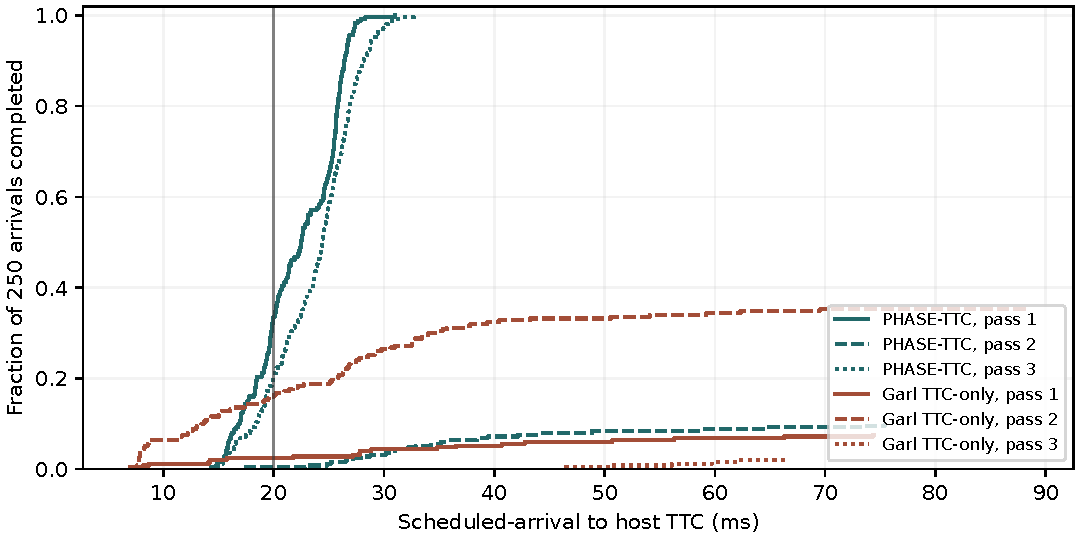
\includegraphics[width=\linewidth]{figures/persistent_latency_cdf.pdf}
\caption{\textbf{Persistent-service responses and coverage.} Each curve uses all 250 offered arrivals as its denominator; an incomplete replay stops below one. The vertical line marks the 20\,ms target; no scheduling or acquisition time is subtracted.}
\end{figure}

\begin{table}[H]
\centering\small
\caption{\textbf{Resident service and stream allocation.} CUDA peaks are reset after initialization and include resident model, history, graph and cache allocations during the stream. Reserved memory is the PyTorch allocator reserve, not additional model parameters. RGB hits count exact feature-cache reuse.}
\begin{tabular}{lrrrrr}
\toprule
Service & Pass & Allocated MiB & Reserved MiB & RGB hits & Misses \\
\midrule
PHASE-TTC & 1 & 2969.4 & 3428.0 & 143 & 107 \\
Garl TTC-only & 1 & 965.8 & 1110.0 & 11 & 8 \\
Garl TTC-only & 2 & 965.8 & 1110.0 & 53 & 36 \\
PHASE-TTC & 2 & 2969.4 & 3428.0 & 12 & 13 \\
PHASE-TTC & 3 & 2969.4 & 3428.0 & 143 & 107 \\
Garl TTC-only & 3 & 965.8 & 1110.0 & 3 & 3 \\
\bottomrule
\end{tabular}

\end{table}

The primary statistic is the median and range of per-pass p95 values. The three replays reuse the same correlated anchors and are not independent training seeds or 750 independent examples. All offered arrivals, unsuccessful outputs, queue drops and source errors remain in the ledgers. A primary complete-service comparison requires 250/250 valid outputs and successful input/native-output parity for every pass; incomplete runs cannot become faster through filtering.

For Garl, a missing RAW packet invalidates contiguous causal history and causes the service to refuse subsequent requests until a fresh replay. These failures remain capacity failures, but they are correlated refusals rather than emitted inaccurate TTC estimates.

The all-anchor reference verification runs after each measured stream, inside the same process command. Its GPU workload differs between models: Garl's reference executes the full auxiliary-decoder graph. No cooldown is enforced between commands, so reference work can affect the power, thermal and cache state encountered by the next service. The recorded telemetry documents but does not remove this confound. Consequently, these short desktop runs support workload-specific coverage and response observations, not a causal ranking of model speed or an attribution of failures to temperature, background load, or architecture.

\subsection{Evidence and scope}

An initial three-pass comparison used persistent Garl with eager native GPU execution. Queue losses motivated a prospective second execution protocol with separate fixed-shape CUDA graphs for Garl's RGB branch and event/fusion branch, analogous to PHASE's existing graph optimization. The second protocol keeps the cohort, rate, queue and model arithmetic fixed; all three new passes are retained. The first protocol is preserved below, including incomplete PHASE runs. It is not removed to obtain a favorable comparison.

\begin{table}[H]
\centering\small
\caption{\textbf{Earlier eager-Garl protocol, all outcomes.} Complete p95 (ms) is shown only for a fully covered replay. PHASE uses its original optimized service in both protocols.}
\begin{tabular}{lrrrrr}
\toprule
Service & Pass & Outputs & Drops & Errors & Complete p95 \\
\midrule
PHASE-TTC & 1 & 250/250 & 0 & 0 & 31.88 \\
Garl TTC-only & 1 & 29/250 & 2 & 219 & --- \\
Garl TTC-only & 2 & 61/250 & 2 & 187 & --- \\
PHASE-TTC & 2 & 247/250 & 1 & 2 & --- \\
PHASE-TTC & 3 & 169/250 & 1 & 80 & --- \\
Garl TTC-only & 3 & 16/250 & 1 & 233 & --- \\
\bottomrule
\end{tabular}

\end{table}

The directory \texttt{data/persistent\_service\_20261112/} preserves the preregistered protocol and order, source identities, complete per-arrival clocks, service records, independent parity checks and host metadata. The report generator verifies evidence hashes, clock ordering, complete populations and parity before regenerating the tables. Historical query-oriented API measurements remain archived under \texttt{data/local\_hardware\_20261112/}; their latency values are not used in the article's production-service comparison.

The historical 29.14\,ms p95 remains an earlier PHASE reference. Neither that result nor these short matched replays guarantees a strict 20\,ms deadline, physical-camera timing, sustained multi-object operation, or a new accuracy ranking.

\section{Extended inference study: workload diversity, repetition and queueing}
\label{sec:extended-inference}

This study extends the initial five-second CPLA comparison to six recorded scenarios and 72 independently initialized service passes. Its purpose is to measure the behavior of the complete persistent inference services under repeated causal input, rather than infer deployment performance from parameter counts or a model-only forward pass. Both implementations retain their published weights. No TTC labels are read and no model is retrained. The experiment concerns inference on EvTTC and does not change the eAP accuracy results.

\subsection{Questions and prospective design}

The study asks four separate questions. First, does the response distribution reproduce across fresh processes and different scenes? Second, can each service deliver every update offered at 50\,Hz with a small bounded queue? Third, when buffering prevents an immediate history gap, does outstanding work remain bounded or accumulate into delayed responses? Fourth, do the optimized service outputs agree with independent native inference on the same causal observations? These questions require different statistics: a p95 over surviving outputs alone cannot answer the coverage or stability questions.

The campaign fixes the scenarios, interval-selection rule, repetitions, queue capacities, precision, rest policy and order before timing. It makes four passes per model and scenario with a two-packet queue, followed by two passes with a 64-packet queue. Each repetition alternates the first model in the pair, and the scenario order rotates. Thus each model occupies first position equally often within each queue policy. Every attempt is retained, including initialization failures, acquisition errors, dropped packets and subsequent refusals. The larger queue is a diagnostic of buffering and backlog; it does not establish an acceptable deployment latency.

\subsection{Sensor support and cohort selection}

All 32 physical sequences in the preserved transfer manifest are inspected using event-clock endpoints and causal annotation availability. A fixed 20\,ms grid begins at 700\,ms, or at the first event plus 620\,ms when that is later. The scout records every accepted and rejected slot. It does not inspect TTC, depth, velocity, RGB pixels, model predictions or measured latency when selecting the workload. The complete scout is reconstructed and checked before the campaign is frozen.

Six scenarios are declared to include cars and pedestrians, straight and lateral motion, different road configurations and different speed categories. For each, the longest uninterrupted accepted interval is selected; ties use the earliest interval. Invalid annotation slots are not removed and joined across a gap. The resulting intervals are listed in Table~\ref{tab:extended-cohorts}. This is an input-availability selection rule, not an unbiased random sample of all driving time: scenes and instants without a usable annotated target are outside the timed cohort.

\begin{table}[H]
\centering\footnotesize
\caption{\textbf{Distinct continuous sensor intervals.} Duration is the number of scheduled updates divided by 50; the last anchor is one period before the interval end. The same interval is replayed in each repetition.}
\label{tab:extended-cohorts}
\begin{tabular}{llrrr}
\toprule
ID & Sequence & Start (s) & Updates & Duration (s) \\
\midrule
S1 & CPLA-low & 16.76 & 370 & 7.40 \\
S2 & CCRm-medium-0-overlap-0 & 8.76 & 465 & 9.30 \\
S3 & CCRs-3-low-100-overlap-100 & 6.52 & 452 & 9.04 \\
S4 & CCRs-side-high & 11.98 & 260 & 5.20 \\
S5 & CPNA-high & 19.62 & 155 & 3.10 \\
S6 & CPNAO-high & 13.02 & 277 & 5.54 \\
\bottomrule
\end{tabular}

\end{table}

The longest usable interval is 465 updates, or 9.3\,s. Repeating this interval increases the evidence about run-to-run variation but does not create a longer unique recording. The six scenes are not joined into one synthetic continuous stream, and the experiment does not claim a 60-second uninterrupted sensor test. Each pass resets its process, history and caches and then consumes the complete registered interval.

\begin{table}[H]
\centering\small
\caption{\textbf{Observed RAW workload.} Counts come from the feeder in the first PHASE small-queue pass, including acquired packets later dropped by the consumer queue. Event rate is averaged over the offered interval; the preload archive also contains initialization history and RGB frames.}
\begin{tabular}{lrrrr}
\toprule
Scene & RAW packets & Events (M) & M events/s & Archive MiB \\
\midrule
S1 & 370/370 & 74.94 & 10.13 & 2026 \\
S2 & 465/465 & 135.44 & 14.56 & 3017 \\
S3 & 452/452 & 121.67 & 13.46 & 2834 \\
S4 & 260/260 & 103.46 & 19.90 & 2185 \\
S5 & 155/155 & 73.21 & 23.62 & 1506 \\
S6 & 277/277 & 79.47 & 14.35 & 1889 \\
\bottomrule
\end{tabular}

\end{table}

\subsection{Hardware, initialization and controlled execution choices}

Both services execute on the same NVIDIA RTX 5070 Ti Laptop GPU with 12\,GiB VRAM, on an AMD Ryzen 9 9955HX host with 32\,GiB system memory. The measured environment uses Python 3.11.15, PyTorch 2.11.0 with CUDA 12.8, and driver 591.86. Inference is FP32 with TF32 disabled. Both use two PyTorch CPU threads; PHASE additionally retains its eight RGB preparation workers. Garl uses one inter-op thread. The recorded configurations, rather than nominal hardware specifications alone, define the execution comparison.

Model loading, private RAW preload, the initial 600\,ms event history, synthetic shape priming, graph capture and feeder warmup precede measured arrivals. A fixed 15-second rest follows feeder warmup in both services. Host and GPU state are recorded around this rest, outside the measurement interval. The rest is a reproducible waiting policy, not proof of thermal equilibrium. Desktop scheduling and other host activity remain uncontrolled, and there is no attribution of a slow pass to temperature or a particular background process without direct evidence.

All timed passes finish before any native-reference GPU work begins. This removes the specific interleaving of full-decoder reference inference and subsequent timing present in the initial experiment. It does not equalize the architectures' own initialization costs or eliminate all device-state variation. Startup timings and memory envelopes are retained separately. No concurrent GPU experiment is launched by this campaign.

\begin{table}[H]
\centering\small
\caption{\textbf{Observed GPU state after the pre-stream rest.} Ranges are point-in-time observations across attempts, not continuous telemetry or temperature control. They do not identify the cause of an individual delay.}
\begin{tabular}{llrrr}
\toprule
Policy & Model & GPU temperature $^\circ$C & SM MHz & Power W \\
\midrule
bounded & PHASE & 62.0--74.0 & 210.0--1530.0 & 9.1--26.3 \\
bounded & Garl & 62.0--71.0 & 270.0--307.0 & 9.3--11.1 \\
buffered & PHASE & 62.0--65.0 & 255.0--307.0 & 9.4--10.1 \\
buffered & Garl & 63.0--66.0 & 255.0--292.0 & 9.6--10.1 \\
\bottomrule
\end{tabular}

\end{table}

\subsection{Complete persistent pipelines and architectural comparison}

PHASE executes its complete nine-component system: four modality-specific motion producers, two pair heads, two temporal context refiners and the residual fusion head. Its distributed system contains \LocalPhaseParameters{} parameters. The 1,955-parameter residual head is not substituted for the complete model when reporting size. Persistent event prefixes and exact reverse-transport summaries avoid rebuilding shared history, and native query graphs reduce dispatch overhead. RGB region preparation overlaps event execution, while an identity-checked cache reuses previously computed RGB producer features. Agreement of the resulting output chain with native inference is evaluated separately. Temporal readouts and final TTC predictions are recomputed.

Garl's TTC path uses paired RGB and event ResNet-50 backbones, feature fusion and a height-ratio TTC readout. The full checkpoint retains \LocalGarlStoredParameters{} stored parameters, including auxiliary foreground decoders. Those decoders are bypassed during TTC-only service because they do not contribute to the TTC output; they remain enabled in the independent native reference. The previously recorded execution profile counts \LocalGarlTTCParameters{} parameters in the TTC path, compared with \LocalPhaseExecutedParameters{} in called PHASE modules. These are module-execution parameter counts, not FLOPs or an exported pruned checkpoint size.

Garl receives the last two declared causal RGB endpoints and corresponding boxes in the common input contract. Event support is capped at 100\,ms per endpoint and uses the native 20-plane, first-event-relative representation. The actual endpoint interval is retained in the signed height-ratio conversion. Exact paired RGB backbone features may be reused; independent single-frame embeddings are not substituted for the native six-channel paired backbone. Event preparation may reuse unchanged endpoint tensors, but the event backbone, fusion and TTC heads execute on every completed request. Separate CUDA graphs cover the RGB and event/fusion branches. Neither service caches the final TTC output.

The services therefore have different computational structures despite receiving the same released observations. PHASE combines several compact motion and temporal modules and reuses shared history; Garl applies larger spatial backbones to paired sensor representations. Parameter count describes model storage and executed modules, while measured service time also includes ROI preparation, event encoding, memory movement, graph dispatch and synchronization. No FLOP estimate or asymptotic claim is substituted for measured response, and the results do not isolate a single architectural cause of a latency difference.

The local Garl implementation retains causal event packets in a deque and assembles an endpoint window only when required. On a representation-cache miss, its native-compatible CPU path masks the ROI, groups selected events by pixel and temporal plane using a stable sort, constructs the 20-plane time volume, and applies the released sampling convention before transfer to the GPU. PHASE instead advances its persistent event prefixes and queries the required representations on the GPU. These implementation choices are part of the measured pipelines. The results are not lower bounds on what a different numerically compatible Garl preprocessing implementation could achieve, and a long response cannot be attributed to backbone size alone.

The measured instrumentation also differs: Garl computes a prepared-sensor SHA-256 inside each completed call, while PHASE records causal metadata without hashing every prepared tensor. Both share the feeder's newly released frame checksums. This diagnostic overhead remains inside the reported service response; its isolated contribution is not measured or subtracted.

\subsection{Causality, input age and the measurement clock}

The feeder privately preloads RAW bytes, but releases each packet and newly available frame only at its scheduled causal query. Event conversion and copying, frame sealing, annotation validation, ROI preparation, CPU/GPU transfers, complete inference and host delivery remain within the response path. The initial history contains only observations preceding the first query. A supplied annotated region is assumed available at its declared sensor timestamp; object detection and tracking are not measured.

For scheduled arrival $a_i$, completed RAW availability $v_i$, consumer start $s_i$ and host TTC completion $c_i$, the recorded clocks are
\[
 R_i=c_i-a_i,\qquad A_i=c_i-v_i,\qquad S_i=c_i-s_i,
 \qquad Q_i=s_i-v_i.
\]
The primary response $R_i$ includes release lateness, acquisition and queueing. $S_i$ is service time and $Q_i$ is waiting after the payload is available. Subtracting acquisition or queueing would answer a different question. A 50\,Hz input has a 20\,ms period; response latency may exceed one period while throughput remains 50\,Hz if acquisition and service overlap. Conversely, a short model forward does not establish that the whole service keeps up.

Repeated RGB endpoints retain their original timestamps. Reuse is not presented as a new camera observation at every query. Garl's endpoint identities, source age, prepared-input hashes and cache decisions are recorded for each delivered output. PHASE records the causal event windows, RGB observations, geometry and temporal support used by its full prediction chain. The two systems can aggregate their released history differently; equal arrival packets do not imply identical internal representations.

PHASE's event windows end at the current query and can incorporate new events between RGB arrivals. Garl's native-compatible event volumes end at its declared RGB endpoints, so repeated calls can reuse the same underlying pair. Fifty requested outputs per second therefore does not mean fifty distinct RGB observations or independent predictions per second.

\begin{table}[H]
\centering\small
\caption{\textbf{Age of Garl's latest declared RGB endpoint.} Statistics use the independent native reference at every valid anchor, including anchors for which a timed service did not return a TTC. RGB pairs count distinct endpoint identities.}
\begin{tabular}{lrrrr}
\toprule
Scene & Native references & Age range ms & Median ms & RGB pairs \\
\midrule
S1 & 370/370 & 9.18--49.34 & 29.26 & 148 \\
S2 & 465/465 & 9.54--49.76 & 29.65 & 186 \\
S3 & 452/452 & 9.59--49.82 & 29.70 & 181 \\
S4 & 260/260 & 2.83--47.91 & 25.37 & 104 \\
S5 & 155/155 & 7.43--47.62 & 27.51 & 62 \\
S6 & 277/277 & 9.47--49.59 & 29.53 & 111 \\
\bottomrule
\end{tabular}

\end{table}

\subsection{Independent native verification and evidence preservation}

After all 72 timing attempts, each scenario is reread from disk by an independent native reference for each model. The reference is computed once per unique anchor and then compared with every delivered output from every repetition. This avoids repeatedly heating the GPU with the reference between timed passes while still checking all measured predictions. It does not turn repeated timings into independent prediction samples.

For Garl, verification reconstructs full-frame RGB normalization and native event representations, checks the prepared sensor tensor's SHA-256, and compares both raw heights and signed TTC with relative and absolute tolerances of $10^{-5}$. The unmodified native model executes its auxiliary decoders. For PHASE, verification uses the original uncached predictor, checks all three TTC components with its preserved tolerance contract, and compares causal input metadata exactly. PHASE's metadata receipt is not a hash of every prepared tensor or RAW byte; source-stat, annotation and model/source checks supplement numerical parity. That distinction remains explicit.

The model sources, historical service overlay, model inventories, manifests, timed launchers and measurement commands are frozen before timing. The independent native-reference implementation is included in that freeze. Integrity is checked after timing and around native-reference computation, then checked again before evidence archival. Publication regenerates the numerical comparisons from the saved reference and measured prediction records, verifies file hashes, and rejects altered evidence or missing declared attempts. Numerical disagreements are retained as failed checks; they are not converted into successful native validation. Failed reference computations and absent service predictions remain distinct from successful numerical agreement.

A later-added controller waits for the timed campaign to close and invokes the frozen native-reference implementation. Its job list and executed source are recorded after timing; the controller itself was not prospectively frozen in this campaign. The publication sealer is also a later analysis tool. These stages do not alter the measured services or the frozen native-reference arithmetic.

The recorded Git identifier denotes the base checkout. Exact file digests and archived source snapshots identify the executed revision, including the new benchmark launchers; the base commit alone is not presented as containing those new files. The final publication also preserves the byte identity of the archiver actually executed and its supplemental evidence-sealing script.

\subsection{Numerical agreement and admission of performance claims}

The independent references exposed numerical differences beyond the frozen tolerance in some delivered PHASE outputs. The analysis therefore distinguishes complete delivery from admission under the full numerical contract. An admitted run must deliver every scheduled output and pass all required native checks, including intermediate TTC components. A run that delivers every output but fails an intermediate check remains a complete delivery; its full-service p95 is withheld from admitted comparisons. The tolerance and the measured service code are unchanged.

This reporting distinction was made explicit after inspecting the first numerical failures. It is a retrospective accounting clarification, not a changed timing protocol or a relaxed acceptance threshold. The per-pass timing tables retain the measured response distributions, including numerically rejected outputs, with a separate failed-parity count. The aggregate deadline counts likewise describe delivered timing, not the number of fully validated timely predictions.

The frozen PHASE numerical contract uses relative and absolute tolerances of $10^{-5}$ for each of its three TTC outputs. These differences measure agreement with native inference, not error against TTC labels.

For the fused output, 0 of 4,720 delivered comparisons exceed the contract, covering 0 distinct scene/anchor pairs.

For the event output, 0 of 4,720 delivered comparisons exceed the contract, covering 0 distinct scene/anchor pairs.

For the rgb output, 6 of 4,720 delivered comparisons exceed the contract, covering 3 distinct scene/anchor pairs.


\begin{table}[H]
\centering\footnotesize
\caption{\textbf{PHASE component agreement with native inference.} Checks and failures count repeated delivered comparisons; anchors count distinct failed anchors within each scene, and runs count affected repetitions. Maximum errors use all delivered comparisons. Complete delivery alone does not establish numerical admission.}
\begin{tabular}{llrrrrrr}
\toprule
Scene & Output & Checks & Failures & Anchors & Runs & Max abs. s & Max rel. \\
\midrule
S1 & Fused & 993 & 0 & 0 & 0 & 8.11e-06 & 1.74e-06 \\
S1 & Event & 993 & 0 & 0 & 0 & 0.00e+00 & 0.00e+00 \\
S1 & RGB & 993 & 0 & 0 & 0 & 1.34e-05 & 2.68e-06 \\
S2 & Fused & 942 & 0 & 0 & 0 & 3.59e-04 & 7.17e-06 \\
S2 & Event & 942 & 0 & 0 & 0 & 0.00e+00 & 0.00e+00 \\
S2 & RGB & 942 & 6 & 3 & 2 & 1.22e-03 & 2.11e-05 \\
S3 & Fused & 1365 & 0 & 0 & 0 & 4.29e-06 & 6.95e-07 \\
S3 & Event & 1365 & 0 & 0 & 0 & 0.00e+00 & 0.00e+00 \\
S3 & RGB & 1365 & 0 & 0 & 0 & 8.58e-06 & 1.14e-06 \\
S4 & Fused & 532 & 0 & 0 & 0 & 4.29e-06 & 9.52e-07 \\
S4 & Event & 532 & 0 & 0 & 0 & 0.00e+00 & 0.00e+00 \\
S4 & RGB & 532 & 0 & 0 & 0 & 6.68e-06 & 1.43e-06 \\
S5 & Fused & 322 & 0 & 0 & 0 & 6.68e-06 & 1.32e-06 \\
S5 & Event & 322 & 0 & 0 & 0 & 0.00e+00 & 0.00e+00 \\
S5 & RGB & 322 & 0 & 0 & 0 & 1.62e-05 & 2.39e-06 \\
S6 & Fused & 566 & 0 & 0 & 0 & 1.07e-04 & 3.24e-06 \\
S6 & Event & 566 & 0 & 0 & 0 & 0.00e+00 & 0.00e+00 \\
S6 & RGB & 566 & 0 & 0 & 0 & 5.91e-05 & 3.28e-06 \\
\bottomrule
\end{tabular}

\end{table}

\subsection{Small-queue service response across scenarios}

\begin{table}[H]
\centering\small
\caption{\textbf{Primary 50\,Hz service with queue capacity two.} Four repetitions per model and scene. Delivered runs return every offered update; admitted runs additionally pass every native numerical check. Median p95 and its range are reported only when all four runs are admitted; a dash is not zero latency.}
\label{tab:extended-bounded}
\begin{tabular}{llrrrrr}
\toprule
Scene & Model & Delivered & Admitted & Outputs & p95 & p95 range \\
\midrule
S1 & PHASE & 0/4 & 0/4 & 253/1480 & --- & --- \\
S1 & Garl & 0/4 & 0/4 & 12/1480 & --- & --- \\
S2 & PHASE & 0/4 & 0/4 & 12/1860 & --- & --- \\
S2 & Garl & 0/4 & 0/4 & 12/1860 & --- & --- \\
S3 & PHASE & 1/4 & 1/4 & 461/1808 & --- & --- \\
S3 & Garl & 0/4 & 0/4 & 12/1808 & --- & --- \\
S4 & PHASE & 0/4 & 0/4 & 12/1040 & --- & --- \\
S4 & Garl & 0/4 & 0/4 & 12/1040 & --- & --- \\
S5 & PHASE & 0/4 & 0/4 & 12/620 & --- & --- \\
S5 & Garl & 0/4 & 0/4 & 12/620 & --- & --- \\
S6 & PHASE & 0/4 & 0/4 & 12/1108 & --- & --- \\
S6 & Garl & 0/4 & 0/4 & 12/1108 & --- & --- \\
\bottomrule
\end{tabular}

\end{table}

\begin{figure}[H]
\centering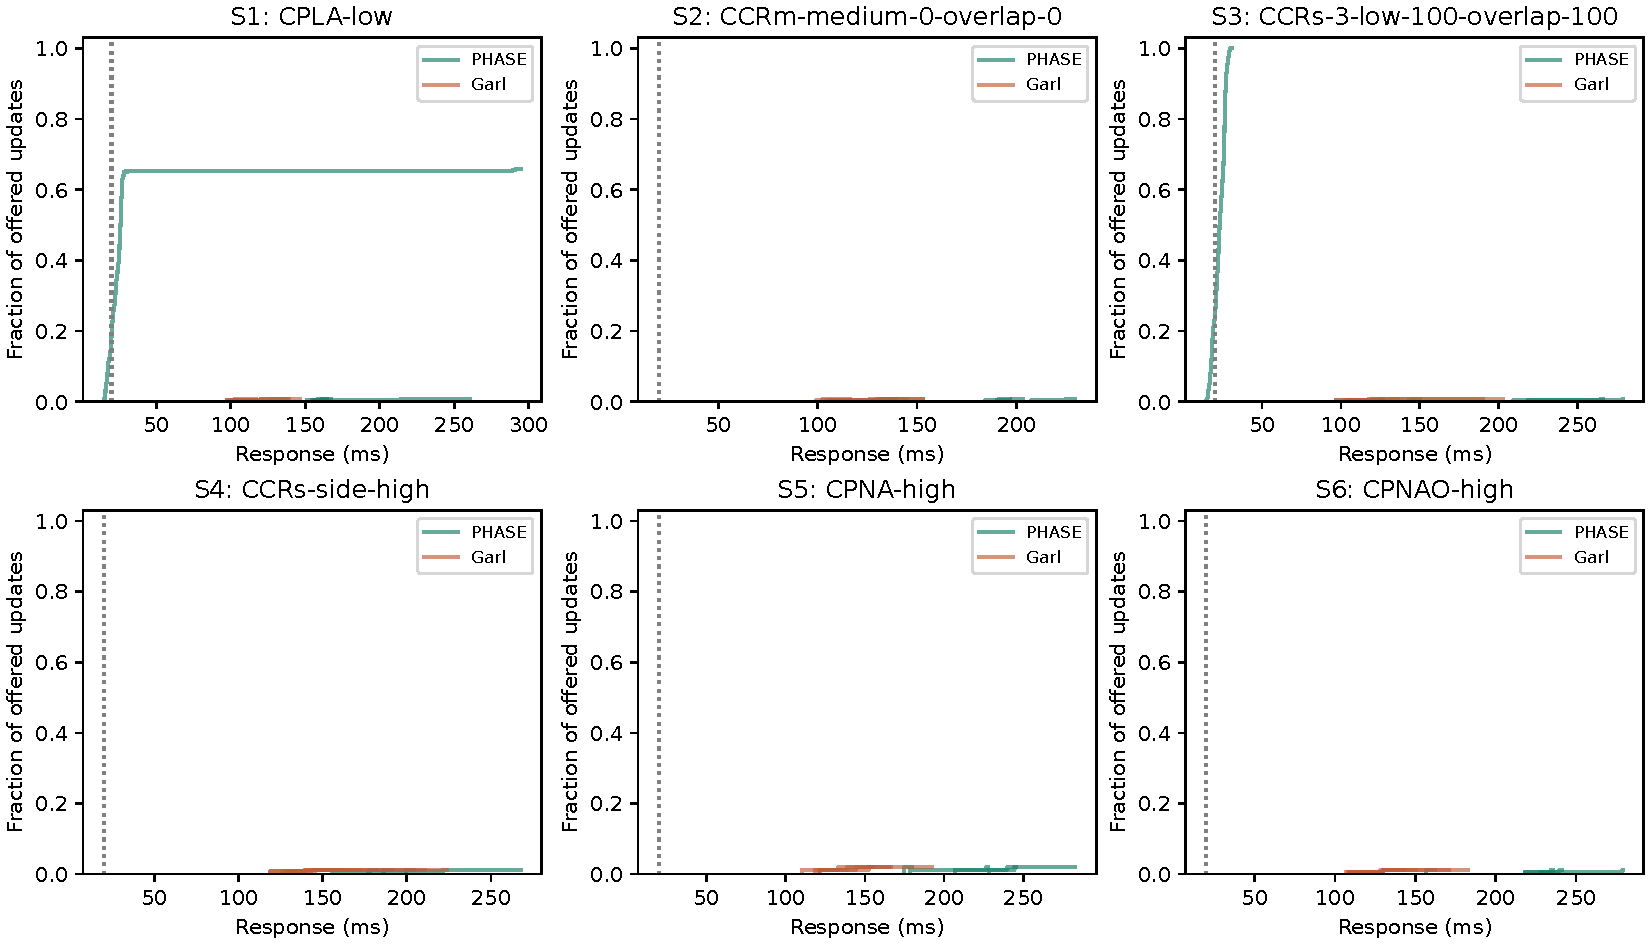
\includegraphics[width=\linewidth]{figures/extended_coverage_cdf.pdf}
\caption{\textbf{Response and coverage in the primary experiment.} Each curve is one attempted replay, with all offered updates in the denominator. Curves that stop below one indicate missing outputs. The dotted line marks 20\,ms.}
\end{figure}

With the two-packet queue, PHASE completed 1/24 full replays and delivered 762/7,916 outputs (9.6\%). Of all offered updates, 178 (2.2\%) completed below 20\,ms. Strict native parity admitted 1/24 full replays; 0 delivered outputs failed at least one required numerical check.

With the two-packet queue, Garl completed 0/24 full replays and delivered 72/7,916 outputs (0.9\%). Of all offered updates, 0 (0.0\%) completed below 20\,ms. Strict native parity admitted 0/24 full replays; 0 delivered outputs failed at least one required numerical check.

With the 64-packet queue, PHASE completed 12/12 full replays and delivered 3,958/3,958 outputs (100.0\%). Of all offered updates, 1,217 (30.7\%) completed below 20\,ms. Strict native parity admitted 10/12 full replays; 6 delivered outputs failed at least one required numerical check.

With the 64-packet queue, Garl completed 7/12 full replays and delivered 3,816/3,958 outputs (96.4\%). Of all offered updates, 429 (10.8\%) completed below 20\,ms. Strict native parity admitted 7/12 full replays; 0 delivered outputs failed at least one required numerical check.


\subsection{Buffering, outstanding work and throughput}

\begin{table}[H]
\centering\small
\caption{\textbf{Buffered diagnostic with queue capacity 64.} Two repetitions per model and scene, retaining the same 50\,Hz input schedule. Full-population p95 includes any accumulated queue delay and requires both runs to be admitted. These measurements are separate from the small-queue primary experiment.}
\label{tab:extended-buffered}
\begin{tabular}{llrrrrr}
\toprule
Scene & Model & Delivered & Admitted & Outputs & p95 & p95 range \\
\midrule
S1 & PHASE & 2/2 & 2/2 & 740/740 & 121.66 & 101.55--141.77 \\
S1 & Garl & 2/2 & 2/2 & 740/740 & 2932.78 & 2850.89--3014.67 \\
S2 & PHASE & 2/2 & 0/2 & 930/930 & --- & --- \\
S2 & Garl & 2/2 & 2/2 & 930/930 & 1741.70 & 1736.81--1746.58 \\
S3 & PHASE & 2/2 & 2/2 & 904/904 & 105.15 & 102.06--108.25 \\
S3 & Garl & 0/2 & 0/2 & 897/904 & --- & --- \\
S4 & PHASE & 2/2 & 2/2 & 520/520 & 226.71 & 225.63--227.78 \\
S4 & Garl & 0/2 & 0/2 & 387/520 & --- & --- \\
S5 & PHASE & 2/2 & 2/2 & 310/310 & 175.53 & 164.74--186.33 \\
S5 & Garl & 2/2 & 2/2 & 310/310 & 4934.71 & 4894.39--4975.03 \\
S6 & PHASE & 2/2 & 2/2 & 554/554 & 103.72 & 94.87--112.56 \\
S6 & Garl & 1/2 & 1/2 & 552/554 & --- & --- \\
\bottomrule
\end{tabular}

\end{table}

\begin{figure}[H]
\centering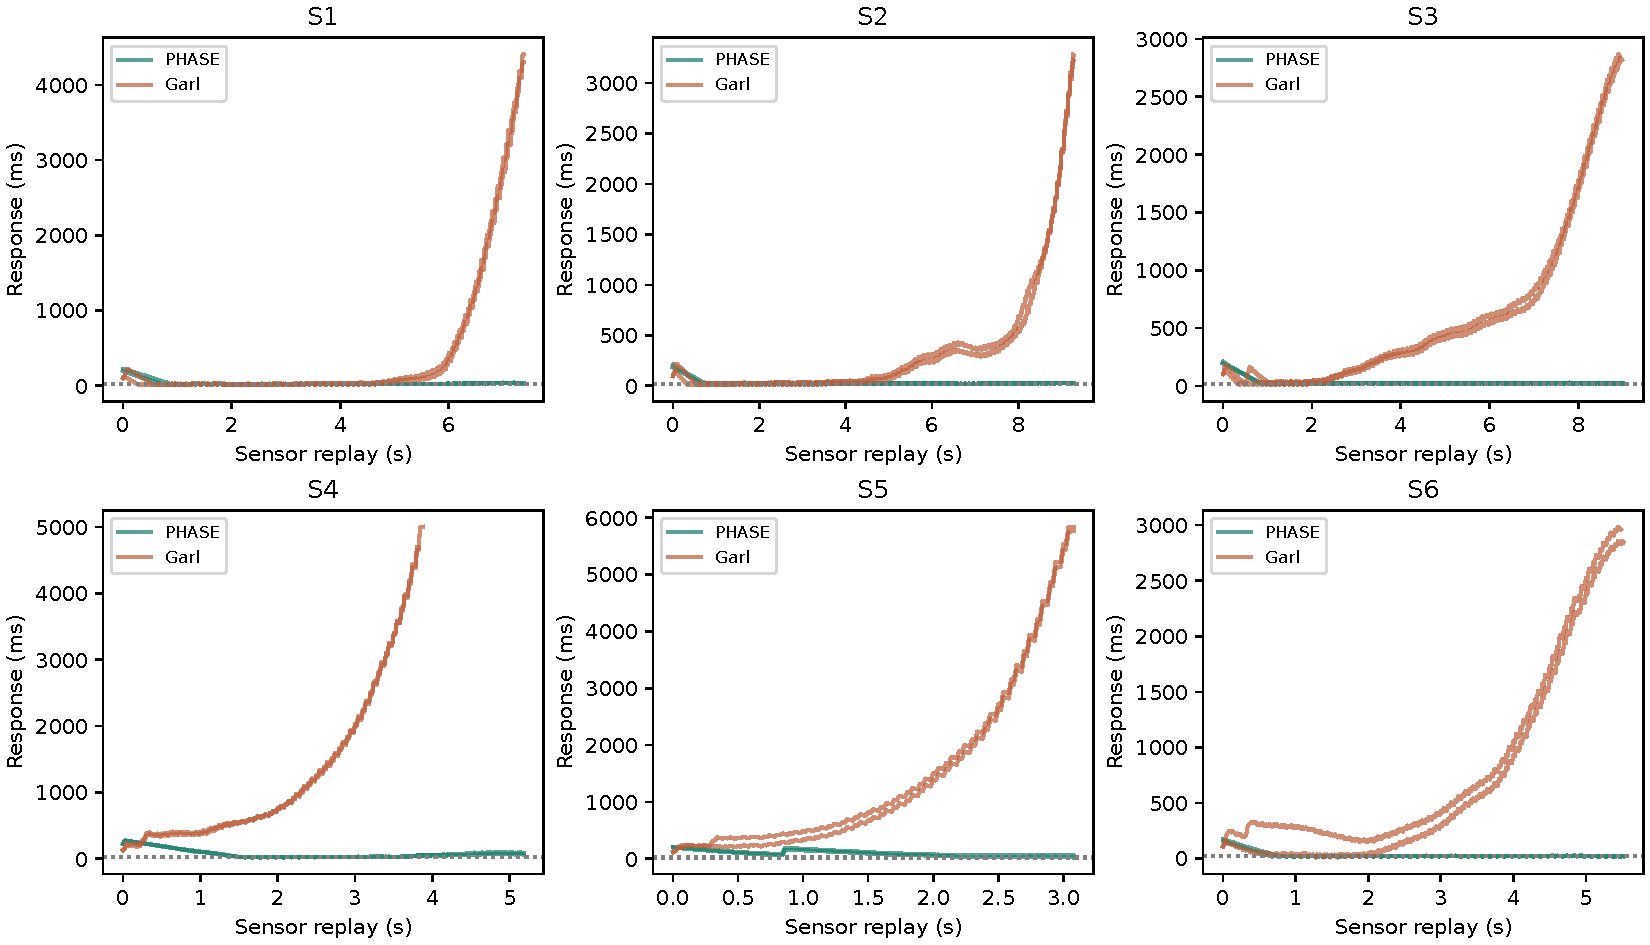
\includegraphics[width=\linewidth]{figures/extended_buffered_traces.pdf}
\caption{\textbf{Response traces with additional buffering.} A rising response trajectory indicates increasing delay relative to sensor time. Missing tails remain missing; no later prediction is invented to complete a curve.}
\end{figure}

The buffered diagnostic distinguishes short overload bursts from the immediate cascade caused by a dropped RAW packet. Both services require contiguous causal history. A missing packet invalidates that history and latches subsequent requests into refusal until a fresh replay; the campaign does not silently refill history, skip sensor time or emit stale TTC. The reported failed responses therefore include correlated refusals, not just independent numerical failures. Recovery behavior is documented rather than changed during this comparison.

Output rate is the number of successful deliveries divided by the interval from the first scheduled arrival to the last successful completion. For an incomplete run this is a diagnostic over its delivered prefix, not sustained capacity for the full offered recording. Drain time measures how far the last valid completion extends beyond the end of the offered interval. Neither quantity is calculated as $1000/\mathrm{p95}$, and neither alone establishes a real-time deadline guarantee. The 64-packet queue can reduce packet loss while allowing responses to become too old for an application.

\subsection{Initial response and later stream behavior}

Inspection of the first completed campaign round showed that an early long service call could fill the small queue and trigger the history-gap cascade. The following breakdown was therefore added retrospectively as a descriptive diagnostic; it is not a prospectively specified primary endpoint or a reason to remove the initial delay. It compares the first response, the p95 of the entire stream, and the p95 of the latter half of scheduled anchors. Each latency column is the median across the two buffered repetitions and is admitted only when both complete the entire interval with native parity. D/A/N gives complete deliveries, admitted runs and declared attempts. The latter half is fixed by anchor index, rather than selected for its measured speed.

\begin{table}[H]
\centering\small
\caption{\textbf{Retrospective initial/later response breakdown, in milliseconds.} Queue capacity 64. The later-window statistic retains its explicit subset definition and is not substituted for complete-stream latency or described as a guaranteed steady-state bound.}
\begin{tabular}{llrrrr}
\toprule
Scene & Model & D/A/N & First response & Full p95 & Latter-half p95 \\
\midrule
S1 & PHASE & 2/2/2 & 208.08 & 121.66 & 36.44 \\
S1 & Garl & 2/2/2 & 99.62 & 2932.78 & 3644.65 \\
S2 & PHASE & 2/0/2 & --- & --- & --- \\
S2 & Garl & 2/2/2 & 96.75 & 1741.70 & 2407.18 \\
S3 & PHASE & 2/2/2 & 199.66 & 105.15 & 27.54 \\
S3 & Garl & 0/0/2 & --- & --- & --- \\
S4 & PHASE & 2/2/2 & 223.12 & 226.71 & 81.17 \\
S4 & Garl & 0/0/2 & --- & --- & --- \\
S5 & PHASE & 2/2/2 & 200.88 & 175.53 & 89.66 \\
S5 & Garl & 2/2/2 & 115.68 & 4934.71 & 5484.29 \\
S6 & PHASE & 2/2/2 & 162.80 & 103.72 & 27.04 \\
S6 & Garl & 1/1/2 & --- & --- & --- \\
\bottomrule
\end{tabular}

\end{table}

\subsection{Memory, initialization and repeated-pass accounting}

\begin{table}[H]
\centering\small
\caption{\textbf{All attempts and service allocation.} CUDA peaks include resident model, persistent state, graph buffers and stream allocations after the counter reset. Values are allocated MiB, not the allocator's additional reserved capacity.}
\begin{tabular}{llrrrr}
\toprule
Queue policy & Model & Delivered & Admitted & Outputs & CUDA peak MiB \\
\midrule
bounded & PHASE & 1/24 & 1/24 & 762/7916 & 2969--2969 \\
bounded & Garl & 0/24 & 0/24 & 72/7916 & 966--966 \\
buffered & PHASE & 12/12 & 10/12 & 3958/3958 & 2969--2969 \\
buffered & Garl & 7/12 & 7/12 & 3816/3958 & 966--966 \\
\bottomrule
\end{tabular}

\end{table}

The RAW feeder declares a conservative 12\,GiB numeric memory envelope, accounting for preload, frame tokens, bounded payloads and scratch space. This is an upper bound rather than measured process RSS, and Python objects, HDF5 internals and output receipts are outside that numeric envelope. A larger queue changes this bound even when immutable frame tokens are shared. Complete startup receipts record RAW preload, model/service initialization, history preparation and graph setup separately from response latency.

\begin{table}[H]
\centering\footnotesize
\caption{\textbf{Initialization and reuse diagnostics.} Preload and model/priming columns give medians across the declared scenes and repetitions, in seconds. Model/priming excludes source audits, RAW history initialization and the fixed rest. Garl graph capture is recorded separately. Cache hits are conditional on attempted model updates, not new sensor frames; reserved MiB is the PyTorch allocator's peak reserve.}
\begin{tabular}{llrrrr}
\toprule
Policy & Model & Preload s & Model/prime s & RGB hits & Reserved MiB \\
\midrule
bounded & PHASE & 2.80 & 9.72 & 446/762 & 3428--3428 \\
bounded & Garl & 2.48 & 2.34 & 32/72 & 1110--1110 \\
buffered & PHASE & 2.61 & 9.91 & 2374/3958 & 3428--3428 \\
buffered & Garl & 2.52 & 2.38 & 2289/3816 & 1110--1110 \\
\bottomrule
\end{tabular}

\end{table}

The following tables retain each repetition instead of pooling correlated windows as if they were independent experiments. Per-pass p50, p95 and p99 are conditional on delivered outputs when coverage is incomplete; only the summary tables apply the all-repetitions full-coverage and native-parity admission rule. The Parity column counts delivered updates failing at least one required numerical check; it is separate from missing or refused outputs. Repetitions measure execution variability with fixed trained weights, not variation across training seeds. Six scenes are insufficient for a broad claim about all event-camera workloads, and no window-level confidence interval is used to imply that they are.

\begingroup\footnotesize
\begin{longtable}{llrrrrrrr}
\toprule
Pass & Model & Outputs & p50 & p95 & p99 & Drops & Failed & Parity \\
\midrule
\endhead
Q2 S1 R1 & PHASE & 244/370 & 23.03 & 27.29 & 178.29 & 12 & 114 & 0 \\
Q2 S1 R1 & Garl & 3/370 & 127.12 & 144.71 & 146.28 & 5 & 362 & 0 \\
Q2 S2 R1 & PHASE & 3/465 & 133.16 & 138.70 & 139.20 & 4 & 458 & 0 \\
Q2 S2 R1 & Garl & 3/465 & 129.27 & 150.50 & 152.39 & 5 & 457 & 0 \\
Q2 S3 R1 & PHASE & 452/452 & 23.03 & 27.84 & 29.25 & 0 & 0 & 0 \\
Q2 S3 R1 & Garl & 3/452 & 131.36 & 195.61 & 201.32 & 7 & 442 & 0 \\
Q2 S4 R1 & PHASE & 3/260 & 199.53 & 203.64 & 204.01 & 7 & 250 & 0 \\
Q2 S4 R1 & Garl & 3/260 & 145.48 & 204.50 & 209.75 & 8 & 249 & 0 \\
Q2 S5 R1 & PHASE & 3/155 & 239.72 & 278.52 & 281.97 & 12 & 140 & 0 \\
Q2 S5 R1 & Garl & 3/155 & 138.56 & 153.57 & 154.90 & 5 & 147 & 0 \\
Q2 S6 R1 & PHASE & 3/277 & 239.36 & 240.93 & 241.07 & 9 & 265 & 0 \\
Q2 S6 R1 & Garl & 3/277 & 127.94 & 177.18 & 181.56 & 7 & 267 & 0 \\
Q2 S2 R2 & Garl & 3/465 & 131.17 & 150.88 & 152.63 & 5 & 457 & 0 \\
Q2 S2 R2 & PHASE & 3/465 & 197.07 & 202.68 & 203.18 & 7 & 455 & 0 \\
Q2 S3 R2 & Garl & 3/452 & 119.24 & 134.44 & 135.79 & 4 & 445 & 0 \\
Q2 S3 R2 & PHASE & 3/452 & 264.56 & 266.23 & 266.37 & 11 & 438 & 0 \\
Q2 S4 R2 & Garl & 3/260 & 139.82 & 159.03 & 160.73 & 5 & 252 & 0 \\
Q2 S4 R2 & PHASE & 3/260 & 177.97 & 181.99 & 182.35 & 7 & 250 & 0 \\
Q2 S5 R2 & Garl & 3/155 & 132.92 & 161.83 & 164.40 & 5 & 147 & 0 \\
Q2 S5 R2 & PHASE & 3/155 & 226.56 & 227.51 & 227.59 & 9 & 143 & 0 \\
Q2 S6 R2 & Garl & 3/277 & 129.57 & 148.17 & 149.82 & 5 & 269 & 0 \\
Q2 S6 R2 & PHASE & 3/277 & 234.12 & 235.14 & 235.23 & 9 & 265 & 0 \\
Q2 S1 R2 & Garl & 3/370 & 119.98 & 136.10 & 137.53 & 4 & 363 & 0 \\
Q2 S1 R2 & PHASE & 3/370 & 213.91 & 255.96 & 259.70 & 10 & 357 & 0 \\
Q2 S3 R3 & PHASE & 3/452 & 278.24 & 278.80 & 278.85 & 11 & 438 & 0 \\
Q2 S3 R3 & Garl & 3/452 & 117.34 & 182.77 & 188.59 & 7 & 442 & 0 \\
Q2 S4 R3 & PHASE & 3/260 & 221.28 & 262.92 & 266.62 & 11 & 246 & 0 \\
Q2 S4 R3 & Garl & 3/260 & 139.17 & 215.36 & 222.13 & 9 & 248 & 0 \\
Q2 S5 R3 & PHASE & 3/155 & 174.80 & 179.38 & 179.79 & 6 & 146 & 0 \\
Q2 S5 R3 & Garl & 3/155 & 144.43 & 164.01 & 165.75 & 6 & 146 & 0 \\
Q2 S6 R3 & PHASE & 3/277 & 156.86 & 161.58 & 162.00 & 6 & 268 & 0 \\
Q2 S6 R3 & Garl & 3/277 & 129.98 & 166.71 & 169.97 & 6 & 268 & 0 \\
Q2 S1 R3 & PHASE & 3/370 & 160.98 & 166.50 & 166.99 & 5 & 362 & 0 \\
Q2 S1 R3 & Garl & 3/370 & 102.63 & 115.32 & 116.45 & 3 & 364 & 0 \\
Q2 S2 R3 & PHASE & 3/465 & 224.33 & 229.12 & 229.55 & 9 & 453 & 0 \\
Q2 S2 R3 & Garl & 3/465 & 102.28 & 114.94 & 116.07 & 3 & 459 & 0 \\
Q2 S4 R4 & Garl & 3/260 & 143.31 & 169.29 & 171.59 & 6 & 251 & 0 \\
Q2 S4 R4 & PHASE & 3/260 & 186.28 & 190.79 & 191.19 & 7 & 250 & 0 \\
Q2 S5 R4 & Garl & 3/155 & 152.29 & 188.11 & 191.29 & 7 & 145 & 0 \\
Q2 S5 R4 & PHASE & 3/155 & 244.38 & 245.06 & 245.12 & 10 & 142 & 0 \\
Q2 S6 R4 & Garl & 3/277 & 129.83 & 141.51 & 142.55 & 5 & 269 & 0 \\
Q2 S6 R4 & PHASE & 3/277 & 278.82 & 279.07 & 279.09 & 11 & 263 & 0 \\
Q2 S1 R4 & Garl & 3/370 & 119.94 & 137.35 & 138.89 & 4 & 363 & 0 \\
Q2 S1 R4 & PHASE & 3/370 & 158.25 & 163.81 & 164.30 & 5 & 362 & 0 \\
Q2 S2 R4 & Garl & 3/465 & 125.86 & 142.90 & 144.42 & 5 & 457 & 0 \\
Q2 S2 R4 & PHASE & 3/465 & 190.76 & 196.23 & 196.72 & 7 & 455 & 0 \\
Q2 S3 R4 & Garl & 3/452 & 124.17 & 126.28 & 126.47 & 4 & 445 & 0 \\
Q2 S3 R4 & PHASE & 3/452 & 144.26 & 149.57 & 150.04 & 5 & 444 & 0 \\
Q64 S1 R1 & PHASE & 370/370 & 22.90 & 101.55 & 173.70 & 0 & 0 & 0 \\
Q64 S1 R1 & Garl & 370/370 & 30.53 & 2850.89 & 4089.93 & 0 & 0 & 0 \\
Q64 S2 R1 & PHASE & 465/465 & 22.76 & 72.18 & 157.84 & 0 & 0 & 3 \\
Q64 S2 R1 & Garl & 465/465 & 64.37 & 1736.81 & 2967.25 & 0 & 0 & 0 \\
Q64 S3 R1 & PHASE & 452/452 & 22.52 & 108.25 & 184.94 & 0 & 0 & 0 \\
Q64 S3 R1 & Garl & 450/452 & 321.58 & 2407.23 & 2769.95 & 2 & 0 & 0 \\
Q64 S4 R1 & PHASE & 260/260 & 50.76 & 227.78 & 263.92 & 0 & 0 & 0 \\
Q64 S4 R1 & Garl & 195/260 & 697.87 & 4014.08 & 4997.96 & 41 & 24 & 0 \\
Q64 S5 R1 & PHASE & 155/155 & 94.91 & 186.33 & 199.87 & 0 & 0 & 0 \\
Q64 S5 R1 & Garl & 155/155 & 841.74 & 4975.03 & 5833.15 & 0 & 0 & 0 \\
Q64 S6 R1 & PHASE & 277/277 & 22.14 & 94.87 & 143.81 & 0 & 0 & 0 \\
Q64 S6 R1 & Garl & 277/277 & 209.91 & 2693.97 & 2843.05 & 0 & 0 & 0 \\
Q64 S2 R2 & Garl & 465/465 & 102.54 & 1746.58 & 2937.89 & 0 & 0 & 0 \\
Q64 S2 R2 & PHASE & 465/465 & 22.48 & 90.81 & 183.41 & 0 & 0 & 3 \\
Q64 S3 R2 & Garl & 447/452 & 352.19 & 2383.48 & 2800.28 & 3 & 2 & 0 \\
Q64 S3 R2 & PHASE & 452/452 & 22.71 & 102.06 & 173.07 & 0 & 0 & 0 \\
Q64 S4 R2 & Garl & 192/260 & 680.78 & 3860.29 & 4463.59 & 43 & 25 & 0 \\
Q64 S4 R2 & PHASE & 260/260 & 47.62 & 225.63 & 260.53 & 0 & 0 & 0 \\
Q64 S5 R2 & Garl & 155/155 & 707.58 & 4894.39 & 5755.52 & 0 & 0 & 0 \\
Q64 S5 R2 & PHASE & 155/155 & 71.68 & 164.74 & 190.02 & 0 & 0 & 0 \\
Q64 S6 R2 & Garl & 275/277 & 329.94 & 2774.32 & 2957.74 & 1 & 1 & 0 \\
Q64 S6 R2 & PHASE & 277/277 & 23.11 & 112.56 & 161.21 & 0 & 0 & 0 \\
Q64 S1 R2 & Garl & 370/370 & 31.25 & 3014.67 & 4181.92 & 0 & 0 & 0 \\
Q64 S1 R2 & PHASE & 370/370 & 23.28 & 141.77 & 208.67 & 0 & 0 & 0 \\
\bottomrule
\end{longtable}

\endgroup

\begingroup\footnotesize
\begin{longtable}{llrrrrr}
\toprule
Pass & Model & Service p95 & Queue p95 & $<20$ ms & Outputs/s & Drain ms \\
\midrule
\endhead
Q2 S1 R1 & PHASE & 20.73 & 6.26 & 67/370 & 47.3 & 0.0 \\
Q2 S1 R1 & Garl & 90.53 & 103.77 & 0/370 & 16.1 & 0.0 \\
Q2 S2 R1 & PHASE & 121.27 & 117.93 & 0/465 & 18.0 & 0.0 \\
Q2 S2 R1 & Garl & 92.64 & 105.87 & 0/465 & 15.6 & 0.0 \\
Q2 S3 R1 & PHASE & 21.62 & 6.77 & 111/452 & 50.0 & 0.0 \\
Q2 S3 R1 & Garl & 97.11 & 103.57 & 0/452 & 12.4 & 0.0 \\
Q2 S4 R1 & PHASE & 179.79 & 181.93 & 0/260 & 12.5 & 0.0 \\
Q2 S4 R1 & Garl & 116.68 & 117.75 & 0/260 & 11.9 & 0.0 \\
Q2 S5 R1 & PHASE & 162.11 & 209.03 & 0/155 & 9.3 & 0.0 \\
Q2 S5 R1 & Garl & 107.14 & 111.89 & 0/155 & 15.4 & 0.0 \\
Q2 S6 R1 & PHASE & 201.71 & 214.15 & 0/277 & 10.7 & 0.0 \\
Q2 S6 R1 & Garl & 98.20 & 100.84 & 0/277 & 13.5 & 0.0 \\
Q2 S2 R2 & Garl & 93.60 & 108.16 & 0/465 & 15.5 & 0.0 \\
Q2 S2 R2 & PHASE & 178.57 & 181.72 & 0/465 & 13.0 & 0.0 \\
Q2 S3 R2 & Garl & 85.76 & 92.68 & 0/452 & 17.0 & 0.0 \\
Q2 S3 R2 & PHASE & 197.64 & 237.41 & 0/452 & 9.9 & 0.0 \\
Q2 S4 R2 & Garl & 105.12 & 111.09 & 0/260 & 14.9 & 0.0 \\
Q2 S4 R2 & PHASE & 160.56 & 160.41 & 0/260 & 13.8 & 0.0 \\
Q2 S5 R2 & Garl & 98.41 & 105.23 & 0/155 & 14.6 & 0.0 \\
Q2 S5 R2 & PHASE & 184.59 & 200.89 & 0/155 & 11.3 & 0.0 \\
Q2 S6 R2 & Garl & 96.56 & 102.18 & 0/277 & 15.8 & 0.0 \\
Q2 S6 R2 & PHASE & 194.21 & 208.42 & 0/277 & 10.9 & 0.0 \\
Q2 S1 R2 & Garl & 86.57 & 97.11 & 0/370 & 16.9 & 0.0 \\
Q2 S1 R2 & PHASE & 142.54 & 187.29 & 0/370 & 10.0 & 0.0 \\
Q2 S3 R3 & PHASE & 191.65 & 247.17 & 0/452 & 9.4 & 0.0 \\
Q2 S3 R3 & Garl & 92.23 & 90.18 & 0/452 & 13.0 & 0.0 \\
Q2 S4 R3 & PHASE & 142.77 & 189.74 & 0/260 & 9.8 & 0.0 \\
Q2 S4 R3 & Garl & 111.02 & 111.68 & 0/260 & 11.4 & 0.0 \\
Q2 S5 R3 & PHASE & 157.88 & 157.81 & 0/155 & 14.0 & 0.0 \\
Q2 S5 R3 & Garl & 104.93 & 116.15 & 0/155 & 14.5 & 0.0 \\
Q2 S6 R3 & PHASE & 141.60 & 139.79 & 0/277 & 15.2 & 0.0 \\
Q2 S6 R3 & Garl & 97.63 & 102.47 & 0/277 & 14.2 & 0.0 \\
Q2 S1 R3 & PHASE & 145.67 & 145.37 & 0/370 & 15.4 & 0.0 \\
Q2 S1 R3 & Garl & 87.39 & 94.06 & 0/370 & 21.0 & 0.0 \\
Q2 S2 R3 & PHASE & 185.07 & 206.48 & 0/465 & 11.3 & 0.0 \\
Q2 S2 R3 & Garl & 89.38 & 93.93 & 0/465 & 21.1 & 0.0 \\
Q2 S4 R4 & Garl & 112.15 & 116.22 & 0/260 & 14.1 & 0.0 \\
Q2 S4 R4 & PHASE & 168.19 & 168.96 & 0/260 & 13.3 & 0.0 \\
Q2 S5 R4 & Garl & 109.05 & 123.30 & 0/155 & 12.9 & 0.0 \\
Q2 S5 R4 & PHASE & 202.50 & 218.59 & 0/155 & 10.5 & 0.0 \\
Q2 S6 R4 & Garl & 96.28 & 102.58 & 0/277 & 16.4 & 0.0 \\
Q2 S6 R4 & PHASE & 197.91 & 248.35 & 0/277 & 9.4 & 0.0 \\
Q2 S1 R4 & Garl & 85.97 & 96.74 & 0/370 & 16.7 & 0.0 \\
Q2 S1 R4 & PHASE & 143.71 & 143.19 & 0/370 & 15.7 & 0.0 \\
Q2 S2 R4 & Garl & 87.42 & 102.53 & 0/465 & 16.2 & 0.0 \\
Q2 S2 R4 & PHASE & 172.77 & 175.35 & 0/465 & 13.4 & 0.0 \\
Q2 S3 R4 & Garl & 90.41 & 97.13 & 0/452 & 18.0 & 0.0 \\
Q2 S3 R4 & PHASE & 131.13 & 128.38 & 0/452 & 16.4 & 0.0 \\
Q64 S1 R1 & PHASE & 23.99 & 79.09 & 153/370 & 50.0 & 3.6 \\
Q64 S1 R1 & Garl & 147.62 & 2749.59 & 114/370 & 31.7 & 4287.1 \\
Q64 S2 R1 & PHASE & 19.35 & 49.89 & 177/465 & 50.0 & 7.5 \\
Q64 S2 R1 & Garl & 85.90 & 1681.29 & 81/465 & 37.0 & 3251.3 \\
Q64 S3 R1 & PHASE & 20.81 & 86.21 & 173/452 & 50.0 & 0.0 \\
Q64 S3 R1 & Garl & 93.64 & 2352.63 & 16/452 & 38.1 & 2757.1 \\
Q64 S4 R1 & PHASE & 27.96 & 205.29 & 18/260 & 49.4 & 63.5 \\
Q64 S4 R1 & Garl & 186.58 & 3925.89 & 0/260 & 21.9 & 3685.4 \\
Q64 S5 R1 & PHASE & 25.20 & 161.96 & 0/155 & 49.4 & 36.0 \\
Q64 S5 R1 & Garl & 284.46 & 4845.24 & 0/155 & 17.4 & 5820.1 \\
Q64 S6 R1 & PHASE & 20.43 & 72.33 & 104/277 & 50.0 & 0.0 \\
Q64 S6 R1 & Garl & 109.58 & 2642.84 & 9/277 & 33.1 & 2828.6 \\
Q64 S2 R2 & Garl & 89.69 & 1690.98 & 77/465 & 37.2 & 3206.2 \\
Q64 S2 R2 & PHASE & 19.51 & 67.72 & 177/465 & 50.0 & 6.4 \\
Q64 S3 R2 & Garl & 91.28 & 2348.36 & 23/452 & 38.0 & 2734.8 \\
Q64 S3 R2 & PHASE & 21.08 & 79.58 & 154/452 & 50.0 & 0.0 \\
Q64 S4 R2 & Garl & 184.99 & 3747.52 & 0/260 & 22.6 & 3308.7 \\
Q64 S4 R2 & PHASE & 27.03 & 204.47 & 26/260 & 49.6 & 40.7 \\
Q64 S5 R2 & Garl & 287.64 & 4770.29 & 0/155 & 17.5 & 5743.8 \\
Q64 S5 R2 & PHASE & 24.56 & 141.67 & 1/155 & 50.0 & 0.0 \\
Q64 S6 R2 & Garl & 108.32 & 2722.23 & 0/277 & 32.6 & 2900.1 \\
Q64 S6 R2 & PHASE & 20.53 & 90.27 & 91/277 & 50.0 & 0.2 \\
Q64 S1 R2 & Garl & 148.11 & 2904.25 & 109/370 & 31.4 & 4388.6 \\
Q64 S1 R2 & PHASE & 24.16 & 116.24 & 143/370 & 49.9 & 12.8 \\
\bottomrule
\end{longtable}

\endgroup

\subsection{Scope of the inference claim}

The expanded evidence supports exact statements about these frozen services, these six annotated EvTTC intervals, this hardware and the declared queue policies. It provides more repetitions and longer unique streams than the initial comparison, while preserving its failures as historical evidence. It does not demonstrate an uninterrupted 60-second stream, physical-camera acquisition, detector latency, multiple independently tracked objects, deployment on a smaller GPU, or eAP streaming performance. The historical 26--29\,ms PHASE p95 values remain valid observations for their original runs, not universal response bounds. Architecture, parameter count, accuracy and deployment response remain separate claims, each tied to its own evidence.
\FloatBarrier

\section{Post-submission controls of 18 November 2026}
\label{sec:post-audit}
\cohortline{DEVELOPMENT FOLDS / 88,744 TRAIN40 queries, 40 sequences / 460 EvTTC queries / no test scoring}

Three controls were run after the claim-scope audit. Each fixed its protocol, arms, metrics, and decision rule in a file written before its comparisons were computed; the protocols are included with the source package, although protocol and results entered version control together, so file times and not commits attest the order. The geometry control is a confirmatory rerun of an earlier exploratory estimate on the same rows, whose approximate size was known when its rule was fixed. None used the private test labels, and no prediction package from these controls has been submitted. The TRAIN40 controls use the out-of-fold rows that fit the released head, grouped by complete sequence. Their levels are not comparable to the test score: the released recipe scores about 85 Overall MiD on these folds and 35.80 on the test server, so differences measured here may not transfer in size.

\subsection{Box-expansion geometry as a head input}
\label{sec:post-audit-geometry}
The benchmark supplies an object region for every query, and its test queries form same-track sequences 100\,ms apart. A causal box-expansion estimate fits the slope of the logarithm of box size, from the square root of area, height, and width, over the same-track regions in the preceding 600\,ms, within the declared 650\,ms budget. We refit the released head recipe under five sequence-disjoint blocks with seeds 7, 13, and 21, with and without these geometry inputs, and with and without a loss weighted by the benchmark's band weights. Table~\ref{tab:post-audit-geometry} reports the official band-weighted score; all values agree with the official scorer to $10^{-12}$.

\begin{table}[htbp]
\centering\small\begin{tabular}{lrrrr}
\toprule
Readout & Inputs & Overall MiD & Crucial & $\Delta$ vs released recipe \\
\midrule
Released recipe, refit in grouped folds & 20 & $85.17\pm0.04$ & 132.4 & --- \\
\quad with band-weighted loss & 20 & $78.01\pm0.10$ & 109.5 & -7.16 $[-9.53,-4.82]$ \\
\quad with box-expansion inputs & 30 & $41.96\pm0.42$ & 56.6 & -43.21 $[-52.64,-34.09]$ \\
\quad with both & 30 & $40.72\pm0.20$ & 50.9 & -44.46 $[-53.91,-35.19]$ \\
RGB fields, box expansion, band loss (selected) & 20 & $41.27\pm0.29$ & 51.1 & -43.90 $[-53.38,-34.55]$ \\
Box expansion only, learned & 10 & $46.09\pm0.10$ & 53.3 & -39.09 $[-49.84,-28.57]$ \\
Box expansion only, fixed estimator & --- & $74.46$ & 100.2 & -10.71 $[-21.22,-0.49]$ \\
Best constant & --- & $198.08$ & 187.9 & +112.91 $[+105.37,+120.24]$ \\
\bottomrule
\end{tabular}

\caption{Head readouts on TRAIN40 development folds; lower is better. Values are the mean and sample standard deviation over three seeds where a fit is involved. Differences are paired sequence-bootstrap estimates against the released recipe, with 10,000 resamples of 40 sequences.}
\label{tab:post-audit-geometry}
\end{table}

Geometry inputs roughly halve the error of the released recipe on these folds. A head that receives only the geometry inputs reaches 46.1; adding the RGB-branch fields brings it to 41.3 and adding the event fields as well to 40.7, so the learned branches contribute about five points beyond supplied-box history, and removing the event fields from the geometry-augmented head costs 0.55 points with an interval of $[0.26,0.88]$. The pre-registered rule, lowest three-seed Overall MiD among variants whose interval against the released recipe excludes zero, with ties within one point resolved toward fewer inputs, selects the variant without event fields. The geometric estimate is not a projection of the label: its correlation with the target phase is 0.93, but its own median error is 34 MiD, and truncated boxes, 15\% of training rows and 10\% of test queries, are markedly worse. Geometry is computable for every test query, with at least five same-track causal frames in 94.6\% of them.

On the benchmark's own training folds the largest available improvement therefore comes from the history of the supplied regions, not from event--RGB fusion or the phase interface. The submitted system does not use box expansion, so this says nothing about the source of its test score.

The size of any test gain is unknown and its sign is not guaranteed. The gap between fold and test levels is concentrated in the crucial band: the released recipe scores 132.4, 39.7, 34.6, and 35.8 in the crucial, small, large, and negative bands on the folds, against 43.52, 28.26, 25.72, and 29.93 for the submitted system on the test server. The selected variant's fold scores in the small, large, and negative bands, 30.1, 33.7, and 33.2, are worse than those test values, and its fold Overall of 41.27 is above the 35.80 already obtained on the test server. One plausible reason, not tested, is that the deployed RGB branch, fitted on forty sequences, is more accurate on test than the fold branches fitted on twenty-four, in which case a head fitted on fold features would weight geometry too heavily. A candidate prediction package for the selected variant exists locally. It differs from the TRAIN40 package by 27.6 MiD on average, a disagreement and not an accuracy, and it has not been submitted.

\subsection{Event history on the training grid}
\label{sec:post-audit-event-history}
Appendix~\ref{sec:field-ranges} documents that the event branch was evaluated with a history grid that differs from training. We rebuilt the event history on the training grid, seven valid slots 50\,ms apart, with every model frozen, and recomputed the event context and the released fusion head on the 460 EvTTC transfer queries. Recomputing the delivered history from raw events reproduces the delivered predictions within $5.7\times10^{-6}$\,s, so arm differences are attributable to the history construction.

\begin{table}[htbp]
\centering\small\begin{tabular}{lrr}
\toprule
Paired contrast & $\Delta$MAE (s) & $\Delta$MiD \\
\midrule
Fusion, matched minus delivered history (primary) & +0.058 $[-0.004,+0.120]$ & +5.2 $[+0.9,+9.1]$ \\
Event context, matched minus delivered & -0.024 $[-0.153,+0.058]$ & +4.8 $[+1.4,+7.9]$ \\
Fusion with matched history minus RGB context & +0.020 $[-0.055,+0.092]$ & +9.9 $[+1.3,+19.4]$ \\
Event context with matched history minus RGB context & +0.501 $[+0.304,+0.722]$ & +75.0 $[+46.9,+107.4]$ \\
\bottomrule
\end{tabular}

\caption{Matched versus delivered event history on 460 development-exposed EvTTC queries; 10,000 complete-recording resamples across 32 recordings. Positive values mean the first arm is worse. MiD is the benchmark's motion-in-depth error, $10^4|\Delta\phi|$, averaged over queries without band weights.}
\label{tab:post-audit-event-history}
\end{table}

The pre-declared rule, written on seconds MAE, returns no measurable effect for the primary contrast: fusion MAE moves from 0.813 to 0.871\,s and its interval includes zero. In the benchmark coordinate the matched history is worse by 5.2 MiD with an interval that excludes zero, fusion improves in 9 of 32 recordings, and a sensitivity arm with all eight slots valid worsens MAE by 0.081\,s with an interval of $[0.002,0.160]$\,s. The matched history is therefore neutral to harmful on this cohort. The matched history does bring the gap and valid-slot fields inside the training support, so the absence of an event benefit is not explained by that mismatch. The event context remains about 0.5\,s worse than the RGB context. An exposure-offset mismatch remains in every arm, since the event anchor coincides with the RGB timestamp on EvTTC, and a model refitted on the inference grid was not tested.

\subsection{History beyond two observations}
\label{sec:post-audit-history}
To isolate the contribution of temporal support, we refit the RGB and event context refiners with history truncated to their $K$ most recent slots, masking older slots identically in fitting and evaluation, under the released rotation scheme, updates, and seeds, and then refit the fusion head with grouped folds. Refitting the untruncated arm reproduces the Overall MiD obtained from the released fusion features within 0.06 points.

\begin{table}[htbp]
\centering\small\begin{tabular}{lrrr}
\toprule
History available to the refiners & Overall MiD & $\Delta$, seed 7 & $\Delta$, three-seed mean \\
\midrule
All retained slots (released) & 85.22 & --- & --- \\
Four most recent slots & 85.84 & +0.62 $[+0.24,+1.01]$ & +0.56 $[+0.25,+0.89]$ \\
Two most recent slots & 88.73 & +3.51 $[+2.67,+4.31]$ & +2.92 $[+2.10,+3.74]$ \\
Current slot only & 90.84 & +5.63 $[+4.61,+6.61]$ & +5.26 $[+4.24,+6.30]$ \\
RGB two slots, events all & 87.58 & +2.36 $[+1.58,+3.20]$ & +2.02 $[+1.28,+2.80]$ \\
RGB all, events two slots & 85.94 & +0.72 $[+0.40,+1.06]$ & +0.64 $[+0.35,+0.96]$ \\
\bottomrule
\end{tabular}

\caption{Fusion-head Overall MiD on TRAIN40 development folds as a function of the history available to the context refiners; seed-7 levels, with paired sequence-bootstrap differences against the released arm.}
\label{tab:post-audit-history}
\end{table}

Restricting both refiners to two slots costs 3.5 points with seed 7 and 2.9 averaged over three seeds; removing history entirely costs 5.6. RGB history accounts for most of the two-slot difference and event history for a smaller, resolved part. Almost all of the benefit is present with four slots. Seconds MAE does not follow the same order: three truncated arms have a lower point MAE than the released arm.

This control bounds the role of history inside PHASE-TTC; it does not reproduce the two-frame regime of the reference method. Each PHASE observation already integrates about 200\,ms of RGB and 300\,ms of events, the producers are fixed, the recipe was developed with full history, and Garl-TTC was not retrained with longer support. On these folds, history beyond two slots explains a few points of an 85-point score, which is small beside the 9.2-point test difference in relative terms but cannot be mapped onto it.

\end{document}
